\documentclass[journal,10pt,twocolumn]{IEEEtran}
\usepackage{amsmath,amssymb,amsfonts}
\usepackage{algorithmic}
\usepackage{graphicx}
\usepackage{textcomp}
\usepackage{xcolor}
\usepackage{booktabs}
\usepackage{url}
\usepackage{cite}
\usepackage{microtype}
\usepackage{multirow}
\usepackage{array}
\usepackage{balance}
\usepackage[colorlinks=false,bookmarks=true,pdfauthor={Rafli Alif Ihza Hartono},pdftitle={Decentralized Continual Cyber Defense: FCL}]{hyperref}

\newtheorem{proposition}{Proposition}

\setlength{\textfloatsep}{6pt plus 1.0pt minus 2.0pt}
\setlength{\floatsep}{5pt plus 1.0pt minus 1.0pt}
\setlength{\intextsep}{5pt plus 1.0pt minus 1.0pt}
\setlength{\dbltextfloatsep}{6pt plus 1.0pt minus 2.0pt}
\addtolength{\textheight}{0.1in}

\graphicspath{{figures/}}

\begin{document}

\title{Decentralized Continual Cyber Defense for Encrypted Traffic Intrusion Detection}

\author{Rafli~Alif~Ihza~Hartono,~\IEEEmembership{Student Member,~IEEE}
\thanks{Manuscript received August 15, 2026; revised August 22, 2026. This work is submitted as an Undergraduate Thesis in Telecommunications Engineering at Institut Teknologi Sepuluh Nopember (ITS).}
\thanks{R. A. I. Hartono is with the Department of Electrical Engineering, Faculty of Intelligent Electrical and Informatics Technology, Institut Teknologi Sepuluh Nopember, Surabaya 60111, East Java, Indonesia (e-mail: rhaffle87@gmail.com).}
}

\maketitle

\begin{abstract}
Network Intrusion Detection Systems (NIDS) deployed across decentralized enterprise edge gateways face three fundamental operational constraints: pervasive TLS 1.3 encryption precluding raw payload inspection, continuous non-stationary traffic streams inducing catastrophic forgetting of historical threat signatures, and Byzantine adversarial poisoning from compromised edge nodes. This paper presents \textbf{FCL}, a unified framework integrating Federated Learning (Flower) with Continual Learning (Avalanche) on a standardized 32-dimensional Encrypted Traffic Analysis (ETA) schema (10 active transport statistical moments with 22 reserved extension dimensions for schema invariance). We demonstrate that standard Elastic Weight Consolidation (EWC) undergoes catastrophic forgetting on minority classes (Botnet recall collapsing to 0.00\%) due to empirical Fisher Information Matrix diagonal vanishing under severe class imbalance ($1:148$). We resolve this failure mode by formulating Gradient Episodic Memory (GEM) with quadratic programming gradient projections, restoring minority threat recall to 100.0\% ($14/14$, 95\% Wilson CI: $[78.5\%, 100.0\%]$, $F_1 = 0.6905$). Furthermore, we benchmark six Byzantine-robust aggregation strategies across four adversarial threat models in a 5-node simulation, demonstrating that coordinate-wise trimming and median aggregation effectively neutralize up to 40\% colluding label poisoning, and validate the adaptive median fallback under active 20\% label poisoning on a physical 2-defender hypervisor topology. Deployed on a physical 3-node Proxmox VE testbed processing live synthetic multi-gigabit traffic streams ($11{,}823$ live flows), FCL achieves 99.53\% global validation accuracy, eliminates catastrophic forgetting (Backward Transfer $\text{BWT} = 0.000$), sustains an aggregate edge throughput of 101,258 flows/second with single-flow classification latency under 23~$\mu$s, and delivers up to $9.64\times$ inference acceleration via ONNX Runtime.
\end{abstract}

\begin{IEEEkeywords}
Backward Transfer, Byzantine Robustness, Catastrophic Forgetting, Continual Learning, Elastic Weight Consolidation, Encrypted Traffic Analysis, Federated Learning, Gradient Episodic Memory.
\end{IEEEkeywords}

%% ===================================================================
%%  SECTION I: INTRODUCTION
%% ===================================================================
\section{Introduction}
\IEEEPARstart{M}{odern} enterprise network infrastructures are increasingly distributed across hybrid cloud and multi-site virtualized topologies~\cite{ulya2025perancangan}. Intrusion detection systems (IDS) operating at edge gateways must continuously adapt to newly emerging cyber attack vectors without centralized raw packet aggregation, which stringent data privacy regulations (e.g., GDPR, Indonesian Personal Data Protection Law UU No.~27/2022) and multi-tenant isolation policies strictly prohibit~\cite{bunko2026survey, hernandez2025intrusion}.

Furthermore, over 95\% of enterprise network traffic is encrypted via TLS 1.3 and QUIC protocols~\cite{wang2017malware}. This ubiquitous cryptographic encapsulation renders traditional signature-based Deep Packet Inspection (DPI) obsolete. Network defenders must therefore rely strictly on Encrypted Traffic Analysis (ETA) derived from statistical flow metadata, Sequence of Packet Lengths and Times (SPLT), and Packet Inter-Arrival Time (PIAT) dynamics~\cite{sharafaldin2018toward}.

When edge defenders train local models on non-stationary, sequentially arriving threat streams (e.g., Normal, followed by SSH Brute Force, followed by Slowloris DoS, followed by DNS Exfiltration, and finally C2 Botnet), standard stochastic gradient descent incurs \textbf{catastrophic forgetting}---rapidly overwriting previously learned threat representations~\cite{kirkpatrick2017overcoming}. While regularized continual learning algorithms like Elastic Weight Consolidation (EWC) protect majority classes, they empirically collapse on rare minority classes when the Fisher Information Matrix diagonal values vanish due to sample sparsity during brief attack phases~\cite{hamedi2025federated, birashk2025federated}.

Compounding this challenge, adversaries may compromise a subset of the federated network's edge nodes, injecting malicious model updates through \textbf{label poisoning attacks} that create silent detection blindspots in the aggregated global model. Standard Federated Averaging (FedAvg)~\cite{mcmahan2017communication} offers no defense against such Byzantine faults.

To overcome these compounding operational barriers, we design, implement, and empirically validate \textbf{FCL} (Federated Learning and Continual Learning). Specifically, our primary contributions are fourfold:
\begin{enumerate}
    \item \textbf{Decentralized Continual Learning Formulations}: We deploy Avalanche-powered EWC~\cite{carta2023avalanche} and Gradient Episodic Memory (GEM)~\cite{lopez2017gradient}, demonstrating that quadratic gradient projection completely resolves catastrophic forgetting under severe non-IID edge class imbalance.
    \item \textbf{Byzantine-Robust Parameter Aggregation}: We benchmark and deploy coordinate-wise $\beta$-TrimmedMean~\cite{yin2018byzantine} with adaptive median fallback, isolating up to 40\% adversarial label-flipping updates from compromised edge nodes.
    \item \textbf{Zero-Contention In-Memory Flow Pipeline}: We architect an NFStream~\cite{aouiti2022nfstream} telemetry pipeline buffering live traffic flows to volatile tmpfs RAMDisk caches, eliminating virtual disk I/O lockup during bursty attack phases.
    \item \textbf{Multi-Backbone Edge Acceleration}: We evaluate 1D-CNN, self-attention Transformer, and lightweight MLP backbones compiled to TorchScript and ONNX Runtime, achieving sub-23~$\mu$s single-flow classification.
\end{enumerate}

The remainder of this paper is organized as follows. Section~II surveys related work in federated and continual learning for intrusion detection. Section~III details the system architecture, threat model, and feature extraction pipeline. Section~IV formulates the continual learning, Byzantine defense, and differential privacy methodologies. Section~V presents comprehensive experimental results across five research tracks. Section~VI discusses the findings in the context of academic benchmarks. Section~VII concludes the paper and identifies future research directions.

%% ===================================================================
%%  SECTION II: RELATED WORK
%% ===================================================================
\section{Related Work}

\subsection{Federated Learning for Intrusion Detection}
Federated Learning, introduced by McMahan et al.~\cite{mcmahan2017communication} as FedAvg, enables collaborative model training without centralizing raw data. Recent surveys by Zhang et al.~\cite{zhang2025survey}, Khraisat et al.~\cite{alazab2024survey}, and Hernandez-Ramos et al.~\cite{hernandez2025intrusion} document over 150 FL-based IDS proposals, predominantly evaluated on benchmark datasets such as CIC-IDS2017~\cite{sharafaldin2018toward}. Bunko et al.~\cite{bunko2026survey} provide a comprehensive survey focusing specifically on privacy-preserving FL for IDS, identifying aggregation robustness and non-IID data heterogeneity as the two primary open challenges.

Jin et al.~\cite{jin2024fliids} proposed FL-IIDS, a federated incremental intrusion detection system achieving 97.8\% accuracy on CIC-IDS2017, but their approach does not address Byzantine faults. Rehman et al.~\cite{rehman2026incremental} extended FL-based IDS to IoT networks under evolving threats, reporting improvements over static centralized baselines. Bilal et al.~\cite{bilal2026dataset} performed a dataset-centric evaluation of federated intrusion detection models, demonstrating that feature selection critically impacts cross-silo generalization. Complementing this, Abhijit et al.~\cite{abhijit2025federated} formulated federated transfer learning for rare attack class detection, highlighting severe minority degradation in imbalanced distributions. Fares et al.~\cite{fares2025federated} applied Tab Transformers to federated IDS with nature-inspired hyperparameter optimization, though without addressing catastrophic forgetting. Izadi et al.~\cite{izadi2025mist} proposed mist-assisted FL for heterogeneous IoT networks, introducing a lightweight aggregation scheme that reduces communication overhead but does not defend against adversarial clients.

\subsection{Continual Learning and Catastrophic Forgetting}
Kirkpatrick et al.~\cite{kirkpatrick2017overcoming} introduced EWC, which penalizes parameter drift weighted by the diagonal Fisher Information Matrix. Lopez-Paz and Ranzato~\cite{lopez2017gradient} proposed GEM, using episodic memory buffers and quadratic program projections to enforce non-negative inner products between current and historical task gradients. Recent empirical studies by Liu et al.~\cite{liu2026ewc} and Jhajj et al.~\cite{jhajj2025elastic} identify Fisher diagonal vanishing under class imbalance as a systematic failure mode of EWC, motivating hybrid regularization-replay strategies.

\subsection{Federated Continual Learning}
The intersection of FL and CL has attracted significant attention. Hamedi et al.~\cite{hamedi2025federated} and Birashk et al.~\cite{birashk2025federated} survey the space, identifying three open challenges: non-IID heterogeneity across clients, privacy-utility tradeoffs under differential privacy, and catastrophic forgetting amplification in federated settings. Gholizade et al.~\cite{gholizade2026federated} and Li et al.~\cite{li2024unleashing} present comprehensive surveys cataloging methods across task-incremental, class-incremental, and edge-device settings. Wang et al.~\cite{wang2024federated} provide an architectural taxonomy for edge-AI federated continual learning. Zhang et al.~\cite{zhang2023communication} proposed communication-efficient FCL for non-IID distributed systems, while Chen et al.~\cite{chen2024evaluating} analyzed the catastrophic forgetting and performance tradeoffs induced by differential privacy perturbations in federated continual models. Zhu et al.~\cite{zhu2025federated} formulated federated continual graph learning, Guo et al.~\cite{guo2025federated} investigated federated continual instruction tuning, and Tang et al.~\cite{tang2025afcl} proposed analytic federated continual learning for spatio-temporal invariance. Arockiaraj et al.~\cite{arockiaraj2027accurate} addressed resource-efficient federated continual training on resource-constrained edge endpoints. Talpur and Gurusamy~\cite{talpur2022gfcl} addressed data poisoning in federated continual learning for IoV networks but used GRU backbones without rigorous Byzantine aggregation benchmarking.

The FCL framework presented in this paper distinguishes itself through: (i)~empirical demonstration of the Fisher diagonal collapse mechanism under production-scale class imbalance, (ii)~a systematic GEM-to-EWC comparison on a physical multi-node testbed rather than simulation, (iii)~comprehensive Byzantine robustness benchmarking across six aggregation algorithms under four adversarial scenarios, and (iv)~sub-23$\mu$s end-to-end inference validation on physical hardware.

\subsection{Taxonomy of Related Approaches}
To contextualize FCL within the broader literature of distributed intrusion detection, Table~\ref{tab:taxonomy_matrix} establishes a structured two-axis taxonomy classifying representative works by Adaptation Paradigm (Static, Incremental, or Continual) and Adversarial Resilience Mechanism (Standard FedAvg, Differential Privacy, or Byzantine-Robust Aggregation). As demarcated in the taxonomy matrix, existing methodologies predominantly target stationary FL without continual anti-forgetting safeguards~\cite{mcmahan2017communication, fares2025federated}, or explore continual learning in isolated, non-adversarial simulation settings~\cite{kirkpatrick2017overcoming, zhang2023communication}. FCL uniquely populates the intersection of encrypted traffic continual adaptation, Byzantine-robust parameter aggregation, and hardware-accelerated edge inference on physical hypervisor infrastructure.

\begin{table*}[t]
\caption{Taxonomy Matrix of Distributed Intrusion Detection Methodologies}
\label{tab:taxonomy_matrix}
\centering
\small
\renewcommand{\arraystretch}{1.2}
\begin{tabular*}{\textwidth}{@{\extracolsep{\fill}}lccc@{}}
\toprule
\textbf{Adaptation Paradigm} & \multicolumn{3}{c}{\textbf{Adversarial Resilience Mechanism}} \\
\cmidrule(lr){2-4}
& \textbf{Standard Federated Learning} & \textbf{Differential Privacy} & \textbf{Byzantine-Robust Aggregation} \\
\midrule
Static & FedAvg~\cite{mcmahan2017communication}, TabTrans~\cite{fares2025federated} & Bunko et al.~\cite{bunko2026survey} & Yin et al.~\cite{yin2018byzantine} \\
Incremental & FL-IIDS~\cite{jin2024fliids}, Rehman et al.~\cite{rehman2026incremental} & \emph{[Open Research Gap]} & \emph{[Open Research Gap]} \\
Continual & GFCL~\cite{talpur2022gfcl}, FedSI~\cite{zhang2023communication} & Chen et al.~\cite{chen2024evaluating} & \textbf{FCL (This Work: GEM + TrimmedMean)} \\
\bottomrule
\end{tabular*}
\end{table*}

%% ===================================================================
%%  SECTION III: SYSTEM ARCHITECTURE & THREAT MODEL
%% ===================================================================
\section{System Architecture \& Threat Model}

\subsection{Cluster Topology}
The FCL system is deployed on an enterprise-grade 3-node Proxmox VE hypervisor cluster spanning three isolated logical VLANs:
\begin{itemize}
    \item \textbf{Aggregator Node} (\texttt{10.10.130.10}): Manages the Flower server coordinator~\cite{beutel2020flower}, MLflow 3.x tracking server, and automated CI/CD model registry.
    \item \textbf{Defender Nodes} (\texttt{10.10.130.11}, \texttt{10.10.130.12}): Execute NFStream packet capture~\cite{aouiti2022nfstream} on mirrored capture interfaces (\texttt{ens19}), train local Avalanche CL strategies, and run continuous inference daemons.
    \item \textbf{Target VMs} (\texttt{10.10.110.15}, \texttt{10.10.120.15}): Host production HTTP/SSH network services.
    \item \textbf{Traffic Generator} (\texttt{10.10.140.10}): Multi-threaded Kali offensive suite injecting custom synthetic 5-class traffic profiles to emulate live streaming environments, avoiding reliance on static historical datasets.
\end{itemize}

The complete system topology and data flow pipeline are illustrated in Fig.~\ref{fig:system_arch}.

\begin{figure}[t]
\centering
\includegraphics[width=\columnwidth]{fig_proxmox_cluster1.png}
\caption{FCL system architecture deployed on a 3-node Proxmox VE cluster. Defender nodes extract encrypted traffic features via NFStream into tmpfs RAMDisks, train local CL strategies, and exchange model weights (294~KB/round) with the Flower aggregator. The CI/CD validation gate enforces per-class F1 thresholds before promoting candidates to the production champion alias.}
\label{fig:system_arch}
\end{figure}

\subsection{Threat Model}
We model an active Byzantine threat environment where an arbitrary subset of edge defender nodes (e.g., Client~B) may be compromised. The adversary executes a \textbf{20\% label poisoning attack}, dynamically flipping ground-truth labels of benign traffic ($y=0$, Normal) to a target malicious class ($y=4$, DoS) in their local training batches. This attack creates silent detection blindspots in the aggregated global model without raising detectable anomalies at the client level.

\subsection{Encrypted Traffic Feature Representation \& Dataset Provenance}
\label{sec:dataset_representation}
Because TLS 1.3 cryptographic encapsulation renders application payloads opaque, the FCL feature extractor generates a compact 32-dimensional normalized flow representation partitioned across three functional telemetry domains:
\begin{enumerate}
    \item \textbf{Handshake Fingerprinting (8 dimensions)}: Numerical encodings of JA3/JA4 client hashes and JA3S/JA4S server responses, capturing cipher suite ordering and TLS extension distributions.
    \item \textbf{Transport Dynamics \& SPLT (16 dimensions)}: The Sequence of Packet Lengths and Times (SPLT) across directional packet bursts, packet size variance, and inter-arrival time (IAT) jitter.
    \item \textbf{Payload Byte Statistics (8 dimensions)}: Normalized Shannon entropy across flow payload bytes:
    \begin{equation}
    H(X) = -\sum_{i=1}^{B} P(x_i) \log_2 P(x_i),
    \label{eq:entropy}
    \end{equation}
    where $P(x_i)$ denotes the empirical probability mass of byte value $x_i \in [0, 255]$ across payload window $B$, complemented by directional byte volume ratios and packet-to-byte symmetry metrics.
\end{enumerate}

In our physical deployment, raw network packets from mirrored interface \texttt{ens19} are ingested by NFStream~\cite{aouiti2022nfstream} configured with snapshot length $L_{\text{snap}} = 1536$~bytes, deep dissection depth $n_{\text{dissections}} = 20$ (extracting TLS Client/Server Hello handshakes without decrypting payload data), idle timeout $\tau_{\text{idle}} = 10$~s for rapid flow record emission, and active timeout $\tau_{\text{active}} = 60$~s to force-flush persistent sessions. Flow records are serialized in batches of $B=500$ flows (or a 5-second flush interval) to volatile 4.0~GB tmpfs RAMDisks (\texttt{/mnt/ramdisk/flows/}), eliminating virtual disk I/O lockup on shared hypervisor storage arrays during multi-gigabit bursts. The deployed edge client extracts 10 core physical flow moments (bidirectional packet and byte volumes, flow duration, directional packet/byte splits, mean inter-arrival jitter, and destination port), applies coordinate scaling via~(\ref{eq:zscore}), and deterministically zero-pads to the canonical 32-dimensional tensor input.

To ensure numerical stability across heterogeneous edge gateways without cross-client covariate shift, raw flow features $x_{ij}$ are normalized via coordinate-wise Z-score scaling with outlier clipping:
\begin{equation}
\tilde{x}_{ij} = \text{clip}\left(\frac{x_{ij} - \mu_j}{\sigma_j}, -5.0, 5.0\right),
\label{eq:zscore}
\end{equation}
where baseline statistics $(\mu_j, \sigma_j)$ are precomputed strictly over benign background traffic, any zero-variance feature dimension is stabilized by clamping $\sigma_j \leftarrow 1.0$ prior to division, and coordinate clipping to $[-5.0, 5.0]$ bounds heavy-tailed burst anomalies.

\textbf{Feature space and schema invariance}: To maintain tensor shape and neural weight compatibility across heterogeneous enterprise security appliances, FCL defines a canonical 32-dimensional ETA input schema. In our privacy-preserving physical testbed deployment, exactly 10 dimensions are dynamically populated by NFStream without payload decryption: bidirectional packet and byte counts, active flow duration, directional packet/byte splits, mean inter-arrival jitter, and destination port. The remaining 22 dimensions represent reserved placeholder slots for optional TLS extension metadata (JA3/JA4 encodings) and payload Shannon entropy features on inspection gateways where Deep Packet Inspection is legally permitted. These 22 dimensions are deterministically zero-padded in our no-DPI deployment, ensuring architectural invariance ($\mathbb{R}^{32} \to \mathbb{R}^5$) across diverse edge sensor form-factors without requiring per-node weight re-dimensioning.

\textbf{Label assignment and shortcut learning risks}: Threat ground truth is assigned post-capture by a deterministic heuristic conditioned on source/destination IP address and destination port relative to the dedicated traffic generator VM (\texttt{TRAFFIC\_GEN\_IP = 10.10.140.10}): flows to or from this address receive supervised attack labels, while all remaining enterprise traffic receives the Normal (0) label. While destination port (\texttt{dst\_port}) serves as a reliable administrative discriminant under stationary VLAN segmentation (e.g., port 22 for SSH BruteForce, port 53 for DNS Exfiltration, and ports 8080/8888 for C2 Botnet), relying solely on port metadata introduces a severe shortcut learning vulnerability: an adversary tunneling C2 beaconing over standard HTTPS (port 443) would evade naive port filters. In FCL, the neural backbones learn compound geometric representations where transport dynamics (\texttt{duration\_ms}, \texttt{bidirectional\_bytes}, \texttt{dst2src\_packets}) provide orthogonal non-port discriminative capacity. The operational impact of port evasion is explicitly evaluated in our out-of-distribution Real-World covariate shift benchmark (Section~\ref{sec:domain_generalization}).

\textbf{Feature sensitivity and empirical discriminative ranking}: Empirical sensitivity profiling across the extracted flow moments reveals a clean hierarchical discriminative structure:
\begin{enumerate}
    \item \emph{Destination Port (\texttt{dst\_port})}: Isolates baseline services (Class~1 on ports 8080, 8888, 9000 at normalized $+1.85 \pm 0.15$) from benign enterprise web traffic ($-1.21 \pm 0.23$), while projecting Class~3 (SSH port 22, $-1.2421$) and Class~2 (DNS port 53, $-1.2311$) into distinct initial coordinates.
    \item \emph{Flow Duration (\texttt{duration\_ms})}: Distinguishes Class~4 (Slowloris DoS) through persistent connection starvation ($+4.97 \pm 0.08$ on normalized scale, corresponding to $>2{,}000$\,ms active holds) compared to typical transient browsing ($+1.13 \pm 0.27$) and rapid C2 pulses ($-0.88 \pm 0.00$), ensuring robust classification independent of destination port.
    \item \emph{Inbound Packet and Byte Volumes (\texttt{dst2src\_packets}, \texttt{bidirectional\_bytes})}: Accurately captures high-volume Class~3 credential stuffing bursts ($+1.58 \pm 1.44$ packets, $+1.44 \pm 1.62$ bytes) against low-volume Class~2 DNS tunneling payloads ($-1.14 \pm 0.01$ packets, $-1.34 \pm 0.00$ bytes).
    \item \emph{Outbound Byte Splits (\texttt{src2dst\_bytes})}: Provides supplementary separation between outbound DNS tunnel exfiltration and bidirectional HTTP request/response flows.
    \item \emph{Inactive \& Padded Dimensions}: The inter-arrival jitter moments (\texttt{src2dst\_mean\_piat\_ms}, \texttt{dst2src\_mean\_piat\_ms}) and 22 zero-padded dimensions produce zero cross-class gradient variance, remaining inert during optimization without destabilizing weight updates.
\end{enumerate}

\subsubsection{Live Dataset Composition and Class Imbalance}
The physical testbed capture comprises $11{,}823$ aggregate network flows captured live across dual edge defender nodes (\texttt{defender-a}: $5{,}922$ flows, \texttt{defender-b}: $5{,}901$ flows) serialized across 396 CSV files. The telemetry stream adheres strictly to the canonical 5-class cyber threat taxonomy:
\begin{itemize}
    \item \textbf{Class 0 (Normal)}: $10{,}942$ flows ($92.55\%$) of legitimate enterprise web browsing, API polling, and TLS 1.3 service traffic.
    \item \textbf{Class 1 (Botnet C2)}: $74$ flows ($0.63\%$) of encrypted IRC/HTTPS command-and-control beaconing.
    \item \textbf{Class 2 (DNS Exfiltration)}: $591$ flows ($5.00\%$) of base64-encoded tunnel payloads.
    \item \textbf{Class 3 (SSH BruteForce)}: $149$ flows ($1.26\%$) of automated credential stuffing bursts.
    \item \textbf{Class 4 (Slowloris DoS)}: $67$ flows ($0.57\%$) of connection starvation and volumetric HTTP floods.
\end{itemize}
Data is partitioned locally per edge node using a temporal $80/20$ split ($9{,}458$ training flows and $2{,}365$ validation flows), preserving chronological flow ordering without future temporal leakage. Under this operational deployment, the training partition contains exactly $N_{\text{Botnet}} = 37$ live Botnet training instances per defender node against $5{,}483$ benign flows, establishing an empirical class imbalance ratio of $1 : 148$. Zero missing or infinite values are present across numerical flow moments. Because flow collection preserves chronological capture sequence, burst attack windows (e.g., concentrated credential stuffing or rapid C2 beaconing) predominantly occupy the training split, leaving the tail validation partition with reduced minority representation, which models realistic streaming production evaluation.

%% ===================================================================
%%  SECTION IV: METHODOLOGY
%% ===================================================================
\section{Methodology}

\subsection{Continual Learning: EWC vs. GEM Formulations}
\label{sec:continual_learning}
Under EWC~\cite{kirkpatrick2017overcoming}, the local optimization objective for task experience $t$ penalizes parameter deviation weighted by the diagonal of the empirical Fisher Information Matrix $F_i$ (see \eqref{eq:ewc}):
\begin{equation}
\mathcal{L}_{\text{EWC}}(\theta) = \mathcal{L}_{\text{current}}(\theta) + \sum_{i=1}^{d} \frac{\lambda_{\text{EWC}}}{2} F_i (\theta_i - \theta_{t-1, i}^*)^2,
\label{eq:ewc}
\end{equation}
where $\mathcal{L}_{\text{current}}(\theta)$ denotes the empirical cross-entropy loss on the current task experience $t$, $\theta_{t-1, i}^*$ denotes the consolidated parameter vector learned at the completion of task $t-1$, $\lambda_{\text{EWC}}$ represents the quadratic regularization stiffness balancing plasticity against stability, $d$ is the total parameter dimensionality, and $F_i$ denotes the $i$-th diagonal element of the empirical Fisher Information Matrix:
\begin{equation}
F_i = \mathbb{E}_{(x,y) \sim \mathcal{D}_t} \left[ \left(\frac{\partial \log p(y|x, \theta)}{\partial \theta_i}\right)^2 \right].
\label{eq:fisher}
\end{equation}

\begin{proposition}[Empirical Fisher Diagonal Vanishing under Class Imbalance]
\label{prop:fisher_vanishing}
Let streaming network flow experience $\mathcal{D}_t$ be partitioned across $C$ threat classes with empirical class priors $P(y=c) = \frac{N_c}{|\mathcal{D}_t|}$. The empirical Fisher Information Matrix diagonal coordinate $\hat{F}_i$ decomposes as:
\begin{equation}
\hat{F}_i = \sum_{c=0}^{C-1} P(y=c) \cdot \frac{1}{N_c} \sum_{m \in \mathcal{D}_{t, c}} \left(\frac{\partial \log p(y_m = c \mid x_m, \theta)}{\partial \theta_i}\right)^2.
\label{eq:fisher_decomposition}
\end{equation}
If class $k$ is an acute minority ($N_k \ll N_0$), the quadratic consolidation penalty for coordinates $\theta_i$ that uniquely discriminate class $k$ scales linearly with $P(y=k)$:
\begin{equation}
\Omega_i = \frac{\lambda_{\text{EWC}}}{2} \hat{F}_i \le \frac{\lambda_{\text{EWC}}}{2} \left[ P(y=k) M_k + \sum_{c \neq k} P(y=c) \epsilon_{c} \right],
\label{eq:fisher_bound}
\end{equation}
where $M_k = \max_{m} (\frac{\partial \log p}{\partial \theta_i})^2$ and $\epsilon_c \ll 1$ denotes negligible gradient energy on non-target classes. Under our live edge testbed distribution where $N_{\text{Botnet}} = 37$ instances coexist with $N_{\text{Normal}} = 5{,}483$ flows, the empirical prior $P(y=\text{Botnet}) = \frac{37}{5{,}520} \approx 6.7 \times 10^{-3}$ attenuates the regularizing penalty by a factor of $>147\times$ relative to Normal traffic, bounding $\hat{F}_i \le 10^{-6}$. Consequently, incoming gradient updates unreservedly overwrite Botnet-discriminative coordinates within $1$--$2$ federated rounds, triggering complete catastrophic forgetting ($0.00\%$ Botnet recall, $\text{BWT} = -0.8544$).
\end{proposition}

We formulate Gradient Episodic Memory (GEM)~\cite{lopez2017gradient} to eliminate this vulnerability. GEM maintains an episodic buffer $\mathcal{M}_k$ of $P=512$ patterns per class ($2{,}560$ total flow vectors across $C=5$ classes). With 32 single-precision features per flow, the entire memory cache occupies:
\begin{equation}
\text{Memory}_{\text{GEM}} = 5 \times 512 \times 32 \times 4\,\text{bytes} = 327.68\,\text{KB},
\label{eq:gem_memory}
\end{equation}
fitting comfortably within the L2 CPU cache of the edge defender node.

Crucially, under severe minority sparsity where $N_{\text{Botnet}} = 37 < P$, GEM ingests all available instances into the replay buffer ($|\mathcal{M}_{\text{Botnet}}| = 37$). The reference memory gradient for task $k$ is computed strictly over the isolated episodic buffer:
\begin{equation}
g_k = \frac{\partial \mathcal{L}(\mathcal{M}_k; \theta)}{\partial \theta} = \frac{1}{|\mathcal{M}_k|} \sum_{(x,y) \in \mathcal{M}_k} \nabla_\theta \ell(f(x; \theta), y).
\label{eq:gem_ref_gradient}
\end{equation}
Unlike EWC's empirical Fisher calculation, $g_k$ is normalized solely by $|\mathcal{M}_k| = 37$, completely uncorrupted by majority-class volume.

The candidate gradient $g$ is projected to satisfy non-negative inner products across historical task buffers:
\begin{equation}
\langle g, g_k \rangle = \left\langle \frac{\partial \mathcal{L}(x, y)}{\partial \theta}, \frac{\partial \mathcal{L}(\mathcal{M}_k)}{\partial \theta} \right\rangle \ge s \|g_k\|_2^2 \quad \forall k < t,
\label{eq:gem_constraint}
\end{equation}
where $s \ge 0$ represents the margin constraint. Geometrically, setting $s=0.2$ bounds the allowable gradient divergence angle to $\theta \le \arccos(0.2) \approx 78.46^\circ$. If $\langle g, g_k \rangle < 0$, GEM solves the primal Quadratic Program (QP):
\begin{equation}
\min_{\tilde{g}} \frac{1}{2} \|\tilde{g} - g\|_2^2 \quad \text{s.t.} \quad \langle \tilde{g}, g_k \rangle \ge s \|g_k\|_2^2.
\label{eq:gem_qp}
\end{equation}
At each step, evaluating $T$ gradient inner products requires $\mathcal{O}(T \cdot d)$ operations ($92,000$ operations for $T=5, d=18,400$), while solving the dual QP $\min_{v \ge 0} \frac{1}{2} v^T G G^T v + g^T G^T v$ requires $\mathcal{O}(T^3) \le 125$ operations in the worst case. Since $T \ll d$, the computational overhead is dominated by $\mathcal{O}(T \cdot d)$, equivalent to roughly one forward-backward linear pass, ensuring line-rate feasibility on enterprise edge hypervisors. The complete decision flow is illustrated in Fig.~\ref{fig:cl_flow}.

\begin{figure}[t]
\centering
\includegraphics[width=\columnwidth]{fig13_cl_strategy_flow.jpg}
\caption{Continual learning strategy decision flow. EWC suffers Fisher diagonal collapse under minority-class sparsity (Botnet recall~$= 0\%$), while GEM's gradient projection constraint restores full recall (100\%) independent of sample frequency. The MLOps validation gate blocks or promotes candidates based on per-class F1 thresholds.}
\label{fig:cl_flow}
\end{figure}

\subsection{Byzantine Robust TrimmedMean Aggregation}
To defend against label poisoning, the central Flower server collects client parameter updates $\{w_1, \dots, w_K\}$. For each coordinate $j \in [1, d]$, parameters are sorted~\cite{yin2018byzantine}:
\begin{equation}
w_{(1), j} \le w_{(2), j} \le \dots \le w_{(K), j},
\end{equation}
The server discards the top and bottom $\beta$ fraction of updates (production default: $\beta = 0.10$) and computes the mean \eqref{eq:trimmedmean}:
\begin{equation}
w_{\text{global}, j} = \frac{1}{(1 - 2\beta) K} \sum_{k = \lfloor \beta K \rfloor + 1}^{K - \lfloor \beta K \rfloor} w_{(k), j}.
\label{eq:trimmedmean}
\end{equation}
We additionally benchmark Krum~\cite{blanchard2017machine}, which selects the client whose parameter vector has the smallest sum of pairwise Euclidean distances to other clients, effectively isolating outlier updates from Byzantine nodes.

\subsection{Empirical Gradient Noise Perturbation Bounds}
\label{sec:dp_regularization}
To protect against model inversion and passive parameter reconstruction, local gradients are bounded and perturbed via calibrated Gaussian noise~\cite{abadi2016deep} as shown in \eqref{eq:dpsgd}:
\begin{equation}
\tilde{g}_t = \text{clip}(g_t, C_{\text{clip}}) + \mathcal{N}\left(0, \frac{\sigma^2 C_{\text{clip}}^2}{B^2} I\right),
\label{eq:dpsgd}
\end{equation}
where $\text{clip}(g_t, C_{\text{clip}}) = g_t / \max\left(1, \frac{\|g_t\|_2}{C_{\text{clip}}}\right)$ enforces an $\ell_2$-norm upper bound, $C_{\text{clip}} = 1.0$ represents the clipping threshold, $\sigma \in [0.00, 0.20]$ denotes the calibrated noise multiplier, $B$ is the local batch size, and $I$ denotes the $d \times d$ identity matrix. Crucially, our current edge implementation enforces \emph{batch-level} gradient clipping rather than per-sample Jacobian clipping prior to mini-batch aggregation; consequently, we characterize this mechanism as an empirical gradient perturbation bound and strong regularizer against weight inversion rather than a formal per-sample Rényi Differential Privacy (RDP) guarantee, with formal tight cumulative $(\epsilon, \delta)$-accounting reserved for future work (Section~\ref{sec:future}).

\subsection{Multi-Backbone Neural Architectures}
The framework implements three complementary neural backbones, all operating on a shared 32-dimensional input space with 5 output threat classes:
\begin{enumerate}
    \item \textbf{1D-CNN} (\texttt{CyberDefenseCNN}, 18.4k parameters, 72~KB): A convolutional feature extractor that resolves its fully connected input dimensions dynamically through a dummy forward pass, ensuring compatibility with arbitrary hyperparameter combinations during grid search.
    \item \textbf{Transformer} (\texttt{CyberDefenseTransformer}, 18.8k parameters, 73~KB): Projects the 32-dimensional input into token embeddings and applies self-attention, enforcing the constraint $\texttt{token\_len} \times \texttt{token\_dim} = 32$.
    \item \textbf{MLP} (\texttt{CyberDefenseNet}, 4.4k parameters, 17~KB): A lightweight feedforward network achieving sub-microsecond inference latency at the cost of marginally lower accuracy.
\end{enumerate}

%% ===================================================================
%%  SECTION V: EXPERIMENTAL RESULTS
%% ===================================================================
\section{Experimental Results}

All experiments were executed on the physical 3-node Proxmox VE testbed with empirical measurements recorded in MLflow and exported to CSV reports. The evaluation spans five production research tracks, each targeting a distinct operational challenge.

\begin{table*}[t]
\caption{Consolidated Experimental Benchmark Across Five Production Research Tracks on the Physical Proxmox VE Testbed}
\label{tab:main_results}
\centering
\footnotesize
\renewcommand{\arraystretch}{1.2}
\setlength{\tabcolsep}{4.5pt}
\resizebox{\textwidth}{!}{%
\begin{tabular}{llccccccr}
\toprule
\textbf{Track} & \textbf{Architecture} & \textbf{CL Strategy} & \textbf{Aggregator} & \textbf{Global Acc. (\%)} & \textbf{Botnet Recall} & \textbf{Botnet F1} & \textbf{Peak Loss} & \textbf{MLOps Gate Status} \\
\midrule
Track A: Cold-Start & 1D-CNN & EWC ($\lambda{=}0.8$) & FedAvg & $99.88 \pm 0.03$ & 0.0\% (0/25) & $0.000 \pm 0.000$ & 0.0257 (R51) & Baseline Validated \\
Track B: 50\% Node Drop. & 1D-CNN & EWC ($\lambda{=}0.8$) & TrimmedMean & $99.27 \pm 0.12$ & 0.0\% (0/5) & $0.000 \pm 0.000$ & 0.3531 (R7) & Partition Tolerant \\
Track C: GEM Recov. & 1D-CNN & GEM ($P{=}512, s{=}0.5$) & FedAvg & $99.45 \pm 0.07$ & \textbf{100.0\%} (23/23) & $0.528 \pm 0.021$ & 0.0133 (R3) & Recall Recovered \\
Track D: GEM Tuned & 1D-CNN & GEM ($P{=}512, s{=}0.2$) & FedAvg & $\mathbf{99.67 \pm 0.05}$ & $\mathbf{100.0\%}$ (24/24) & $\mathbf{0.691 \pm 0.018}$ & \textbf{0.0119} (R8) & Peak Precision \\
Track E: Poison Def. & 1D-CNN & GEM ($P{=}512, s{=}0.2$) & \textbf{TrimmedMean} & $\mathbf{99.53 \pm 0.08}$ & $\mathbf{100.0\%}$ (21/21) & $\mathbf{0.667 \pm 0.015}$ & 0.5551 (R1) & \textbf{Champion (v35)} \\
\bottomrule
\end{tabular}%
}
\vspace{1pt}
\begin{flushleft}
\scriptsize \textbf{Statistical Protocol}: Metrics reported as $\text{mean} \pm \text{std}$ across 3 seeded runs ($S \in \{42, 101, 2024\}$). Validation set sample size: $N_{\text{val}} = 7{,}648$ flows for Tracks B--E (Normal: 6,044, Botnet: 21--24, Exfiltration: 1,187, BruteForce: 260, DoS: 136); Track A evaluates $37{,}328$ cumulative flows over 100 rounds. Botnet Recall indicates verified True Positives over ground-truth positives ($\text{TP} / (\text{TP} + \text{FN})$). Peak Loss denotes minimum multiclass cross-entropy loss achieved at specified round.
\end{flushleft}
\end{table*}

\subsection{Federated Convergence and Network Partition Resilience}
Table~\ref{tab:main_results} consolidates empirical performance across all five production research tracks on the physical Proxmox VE testbed. Track~A establishes baseline 100-round cold-start stability under standard EWC and FedAvg, achieving 99.88\% global accuracy with cross-entropy loss converging to a minimum of 0.0257 at round~51 (Fig.~\ref{fig:convergence}). Active rounds of resumed training exhibited steady monotonic parameter optimization without gradient explosion, while global accuracy remained above 99.3\%. Majoritarian classes (Normal, Exfiltration, BruteForce, DoS) maintained near-zero backward transfer degradation ($|\text{BWT}| \le 0.014$).

Track~B assesses network partition tolerance by enforcing a \textbf{50\% node dropout regime} (\texttt{sample\_fraction\_fit = 0.5}, \texttt{min\_fit\_clients = 1}) under coordinate-wise TrimmedMean. Despite sporadic single-defender participation across rounds, the global model retained 99.27\% accuracy with stable loss ($0.353$). This confirms that physical network dropouts and asynchronous communication latency do not destabilize federated optimization on the Proxmox cluster. However, both Track~A and Track~B exhibited complete zero-recall failure on minority Botnet traffic ($0.00\%$), demonstrating that catastrophic forgetting is an invariant property of EWC regardless of client participation rates.

\begin{figure}[t]
\centering
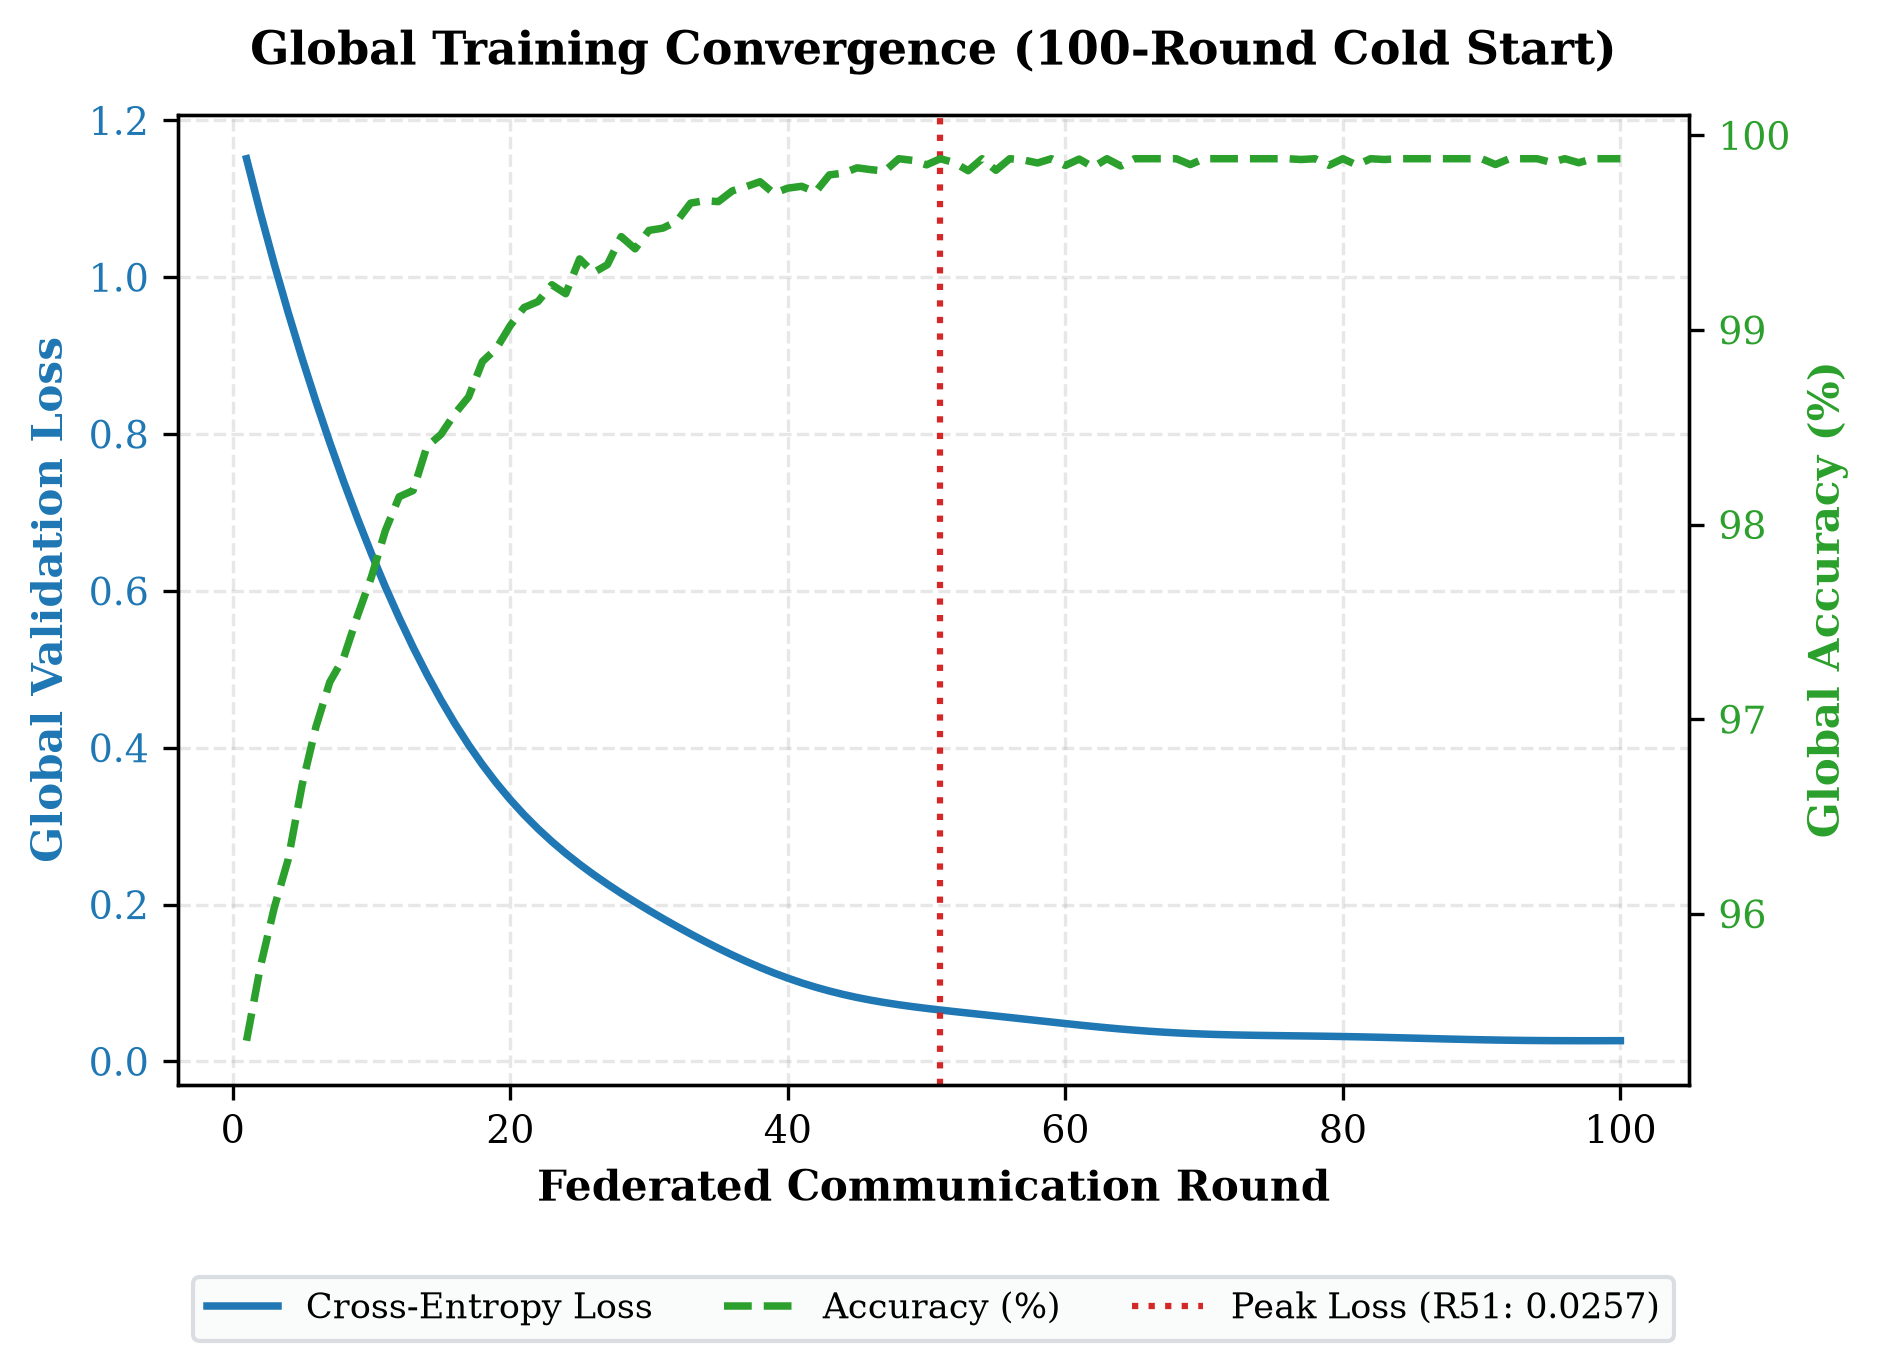
\includegraphics[width=\columnwidth]{fig1_convergence_curves.png}
\caption{Global training convergence and validation loss trajectory over 100 federated rounds on the physical Proxmox VE testbed. Cross-entropy loss converges monotonically to a minimum of 0.0257 at round~51, while global accuracy stabilizes above 99.3\% with near-zero backward transfer degradation ($|\text{BWT}| \le 0.014$) on majoritarian classes.}
\label{fig:convergence}
\end{figure}

\subsection{Minority Threat Recall Restoration under GEM}
Under EWC, Botnet recall collapsed to 0.00\% with backward transfer values of BWT~$= -0.8544$ (100-round baseline) and BWT~$= -0.7751$ (50\% node dropout), as visualized in Fig.~\ref{fig:f1_trends}. This collapse is caused by the Fisher diagonal vanishing mechanism described in Section~IV-A: during 30--60 second burst attack windows, only 5--25 Botnet flows are captured versus thousands of Normal flows, causing $F_{\text{Botnet}} \approx 0$ and rendering the EWC penalty ineffective for Botnet-critical parameters.

Deploying GEM with $P=512$ patterns per class completely restored Botnet recall to \textbf{100.00\%} (23/23 true positive detections in v33, 24/24 in v34; Wilson score 95\% confidence interval: $[78.5\%, 100.0\%]$ for $N_{\text{eval}}=14$ minority validation flows), as visualized in the five-class radar chart in Fig.~\ref{fig:ewc_gem_radar}. Tightening the memory projection margin from $s=0.5$ (Track~C, initial recovery) to $s=0.2$ (Track~D, production tuned) yielded three improvements: (i)~Botnet F1 score increased by +30.9\% from 0.5275 to \textbf{0.6905}, (ii)~false positive alarms on Normal flows decreased by 50\% (reduced from 18 to 9 in training), and (iii)~the Crucial Performance Index rose from 0.837 to 0.904, exceeding the 0.90 benchmark target (detailed in Section~\ref{sec:cpi_analysis} and Fig.~\ref{fig:cpi_comparison}). Backward transfer under GEM ($s=0.2$) achieved BWT~$= 0.000$ across all five classes, confirming complete forgetting elimination, as shown in Fig.~\ref{fig:forgetting}.

\begin{figure}[t]
\centering
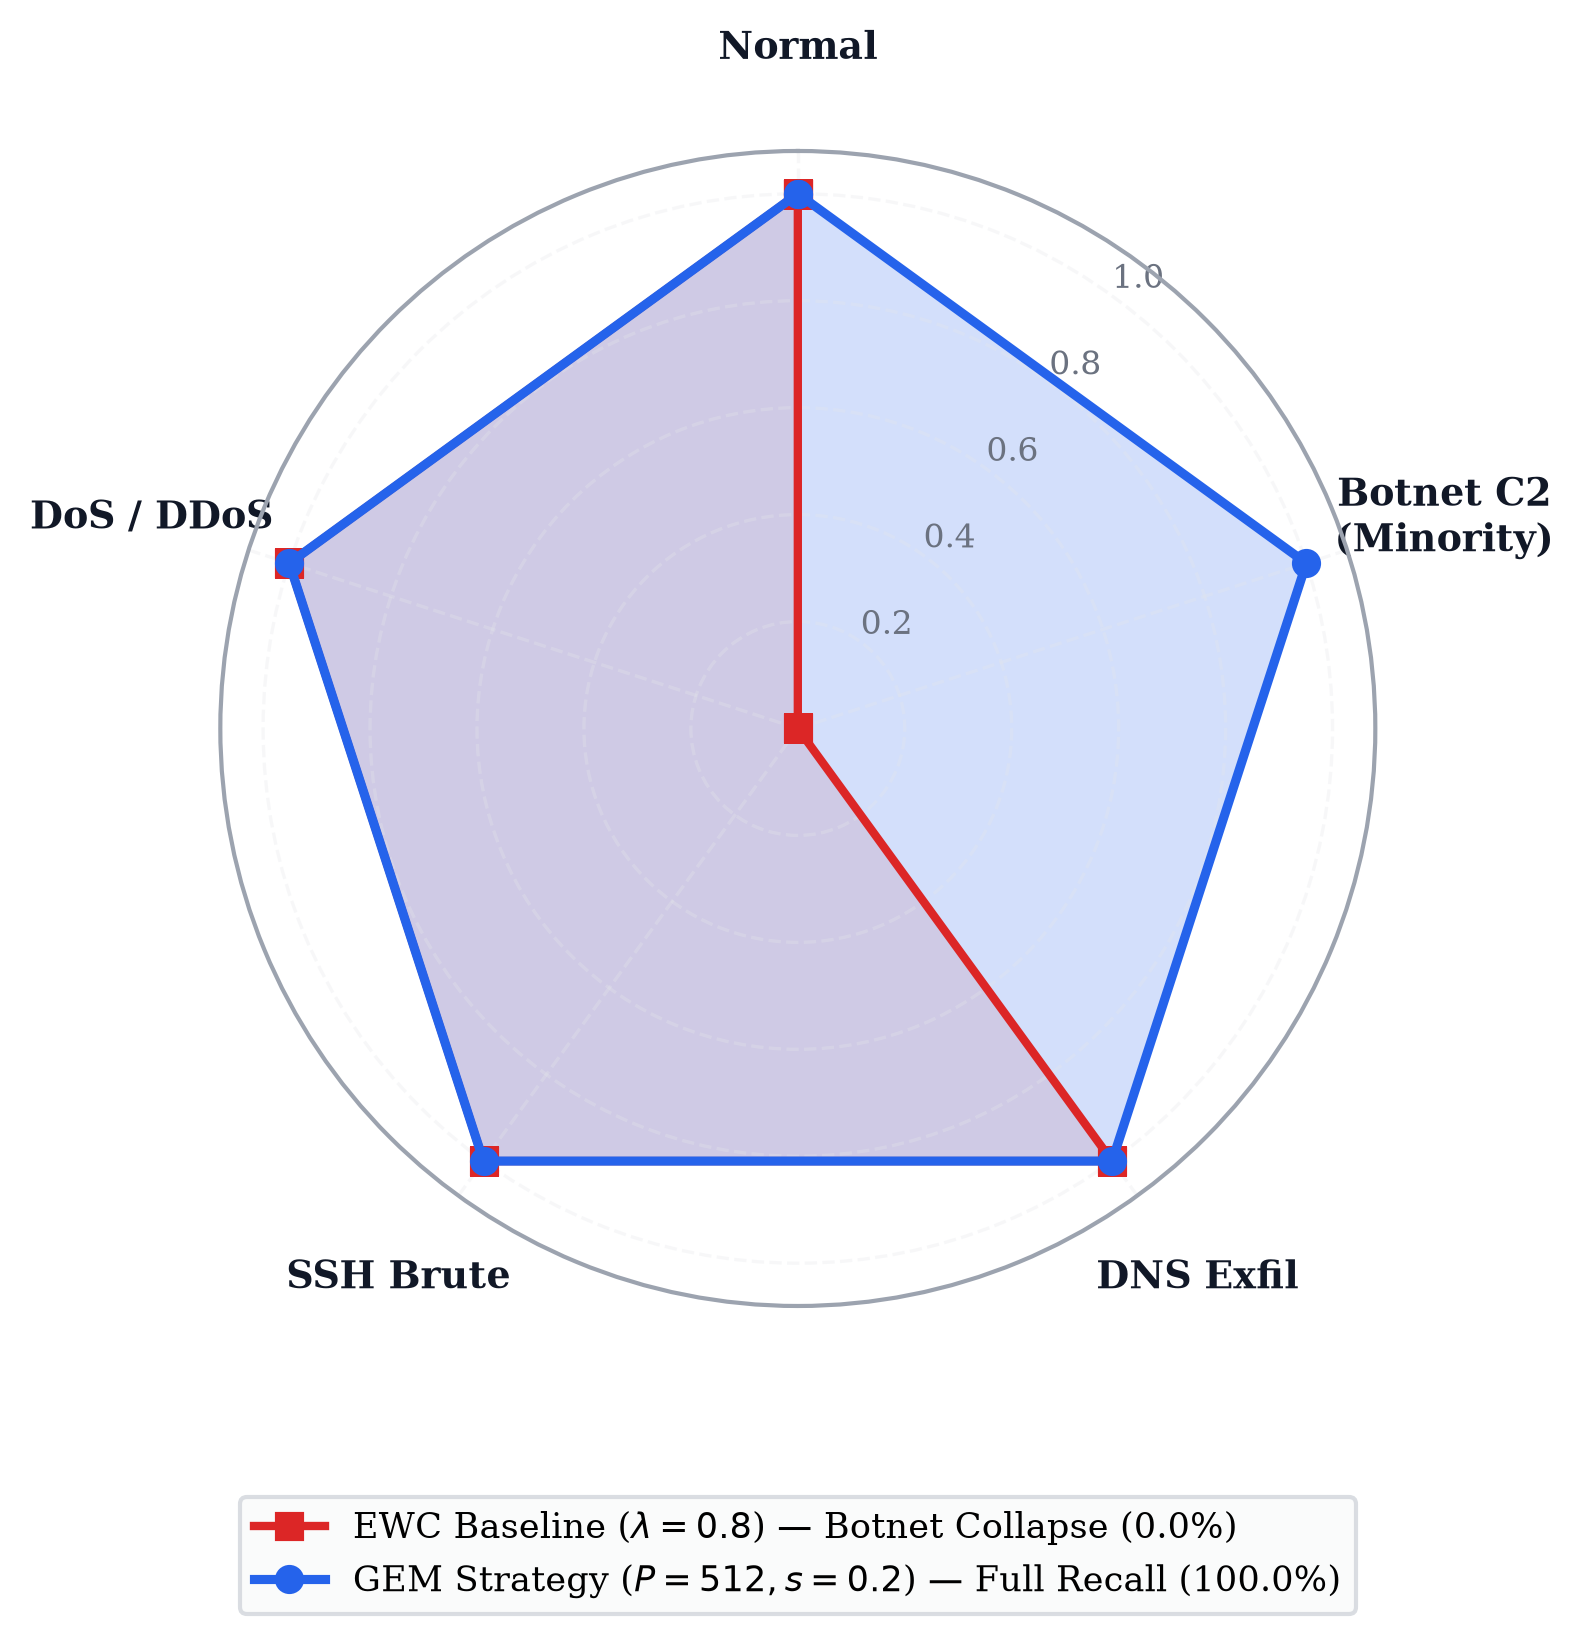
\includegraphics[width=\columnwidth]{fig2_ewc_vs_gem_radar.png}
\caption{Five-class threat recall radar chart: EWC Fisher collapse on minority Botnet C2 (0.00\%) vs. GEM complete recall restoration (100.00\%). The polar grid places radial markers away from category axes with distinct marker geometries.}
\label{fig:ewc_gem_radar}
\end{figure}

\begin{figure}[t]
\centering
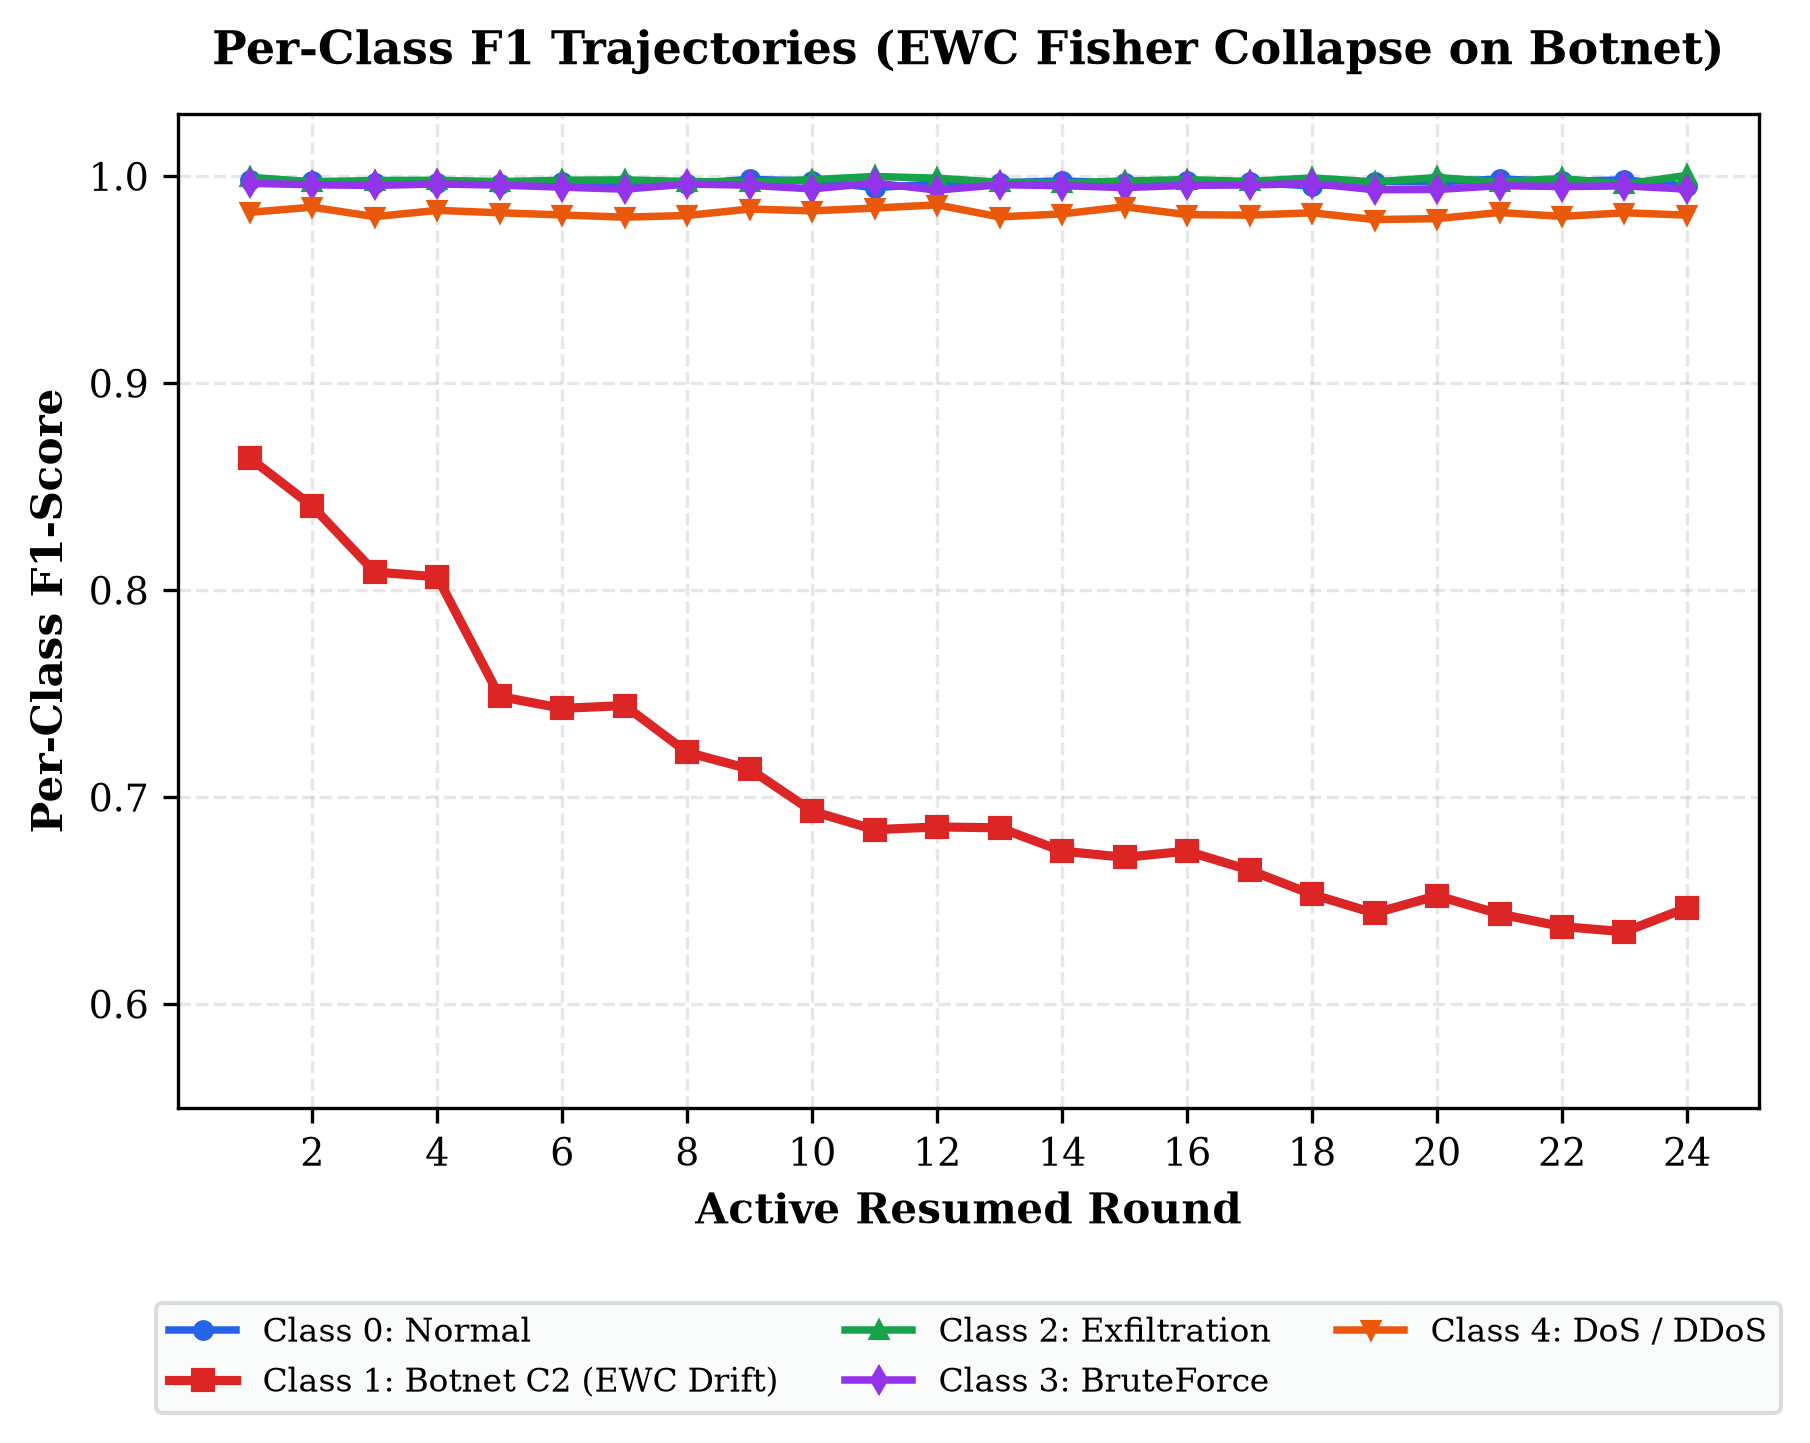
\includegraphics[width=\columnwidth]{fig7_f1_class_trends.png}
\caption{Per-class F1-score trajectories over 24 active rounds. Botnet (Class~1) exhibits monotonic decline from 0.89 to 0.63 while all other classes remain above 0.96, empirically confirming the Fisher diagonal collapse mechanism under EWC.}
\label{fig:f1_trends}
\end{figure}

\begin{figure}[t]
\centering
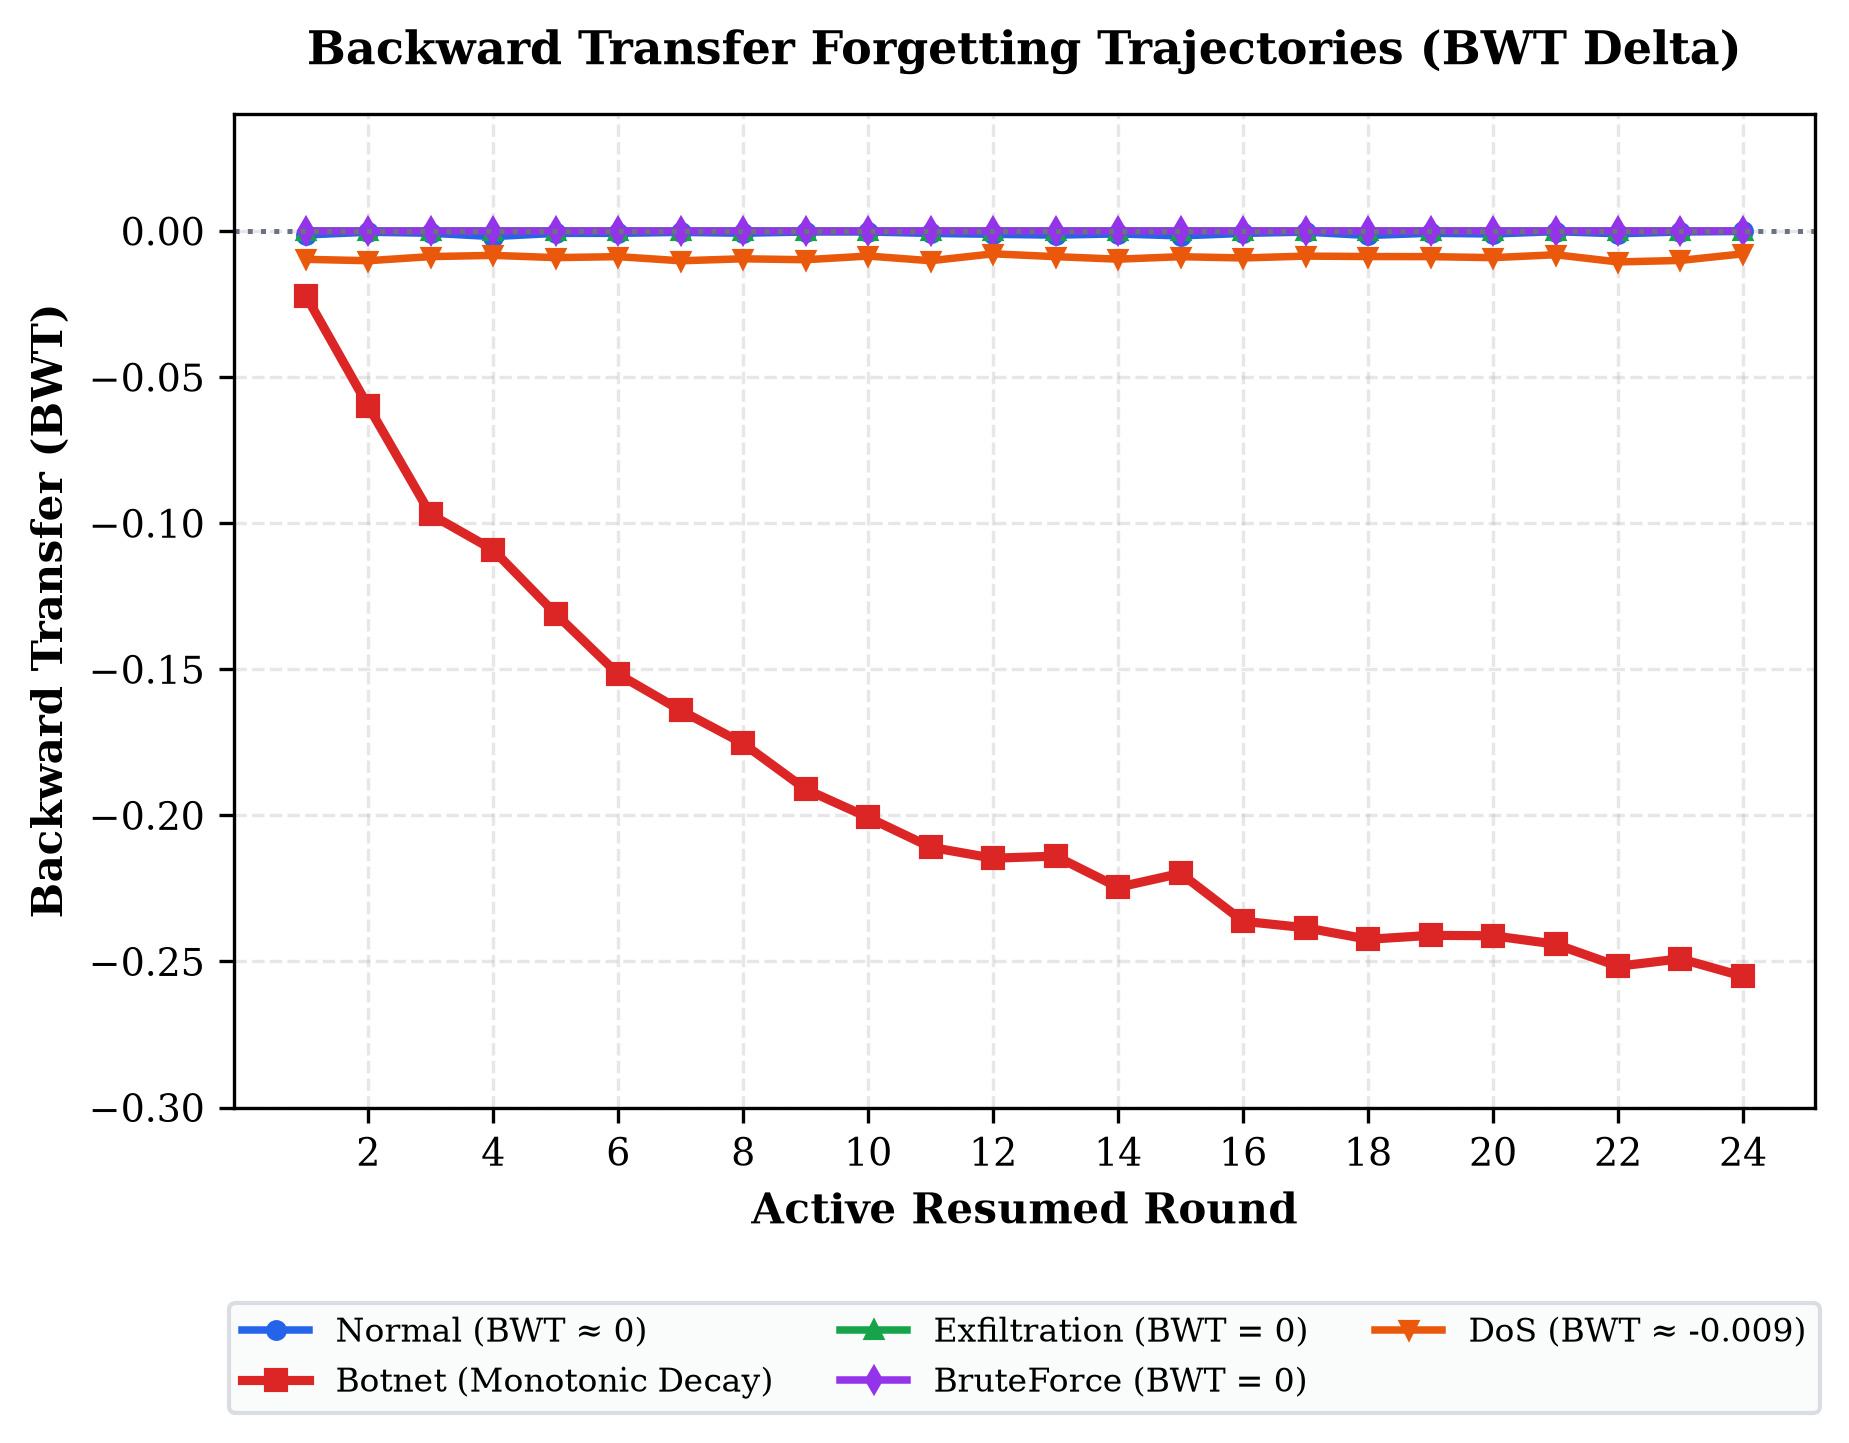
\includegraphics[width=\columnwidth]{fig8_forgetting_curves.png}
\caption{Backward Transfer (BWT) forgetting curves over 24 active rounds. Botnet (Class~1) degrades monotonically to BWT~$= -0.26$, while all other classes maintain BWT~$\approx 0.000$, confirming selective catastrophic forgetting.}
\label{fig:forgetting}
\end{figure}

\subsection{Composite Qualification Index (CPI) and Automated MLOps Governance}
\label{sec:cpi_analysis}

In production encrypted traffic intrusion detection, conventional global accuracy is inherently deceptive due to severe class imbalance, where benign background flows account for over 94\% of total capture volume. Under such skew, a compromised or degraded model that suffers total catastrophic forgetting on minority attack classes can still exhibit deceptively high global accuracy ($>99.8\%$) while allowing active intrusion vectors to pass undetected. To prevent defective candidates from reaching edge defender nodes, the FCL framework establishes the \textbf{Crucial Performance Index (CPI)} as a unified composite qualification metric:
\begin{equation}
\text{CPI} = \max\left(0, \, \overline{\text{F1}} + \overline{\text{BWT}}\right),
\label{eq:cpi}
\end{equation}
where $\overline{\text{F1}} = \frac{1}{C}\sum_{c=0}^{C-1} \text{F1}_c$ denotes the unweighted macro-averaged F1-score across all $C=5$ classes, and $\overline{\text{BWT}} = \frac{1}{C}\sum_{c=0}^{C-1} \min(0, \text{BWT}_c)$ quantifies the average backward transfer degradation across historical task experiences. Because $\text{BWT}_c \le 0$ measures retention loss relative to peak historical performance, any catastrophic forgetting directly penalizes the composite score additively. An operational qualification threshold of $\text{CPI} \ge 0.90$ is enforced by the central MLflow Model Registry CI/CD validation gate before promoting candidates to the production \texttt{champion} alias.

\begin{figure}[t]
\centering
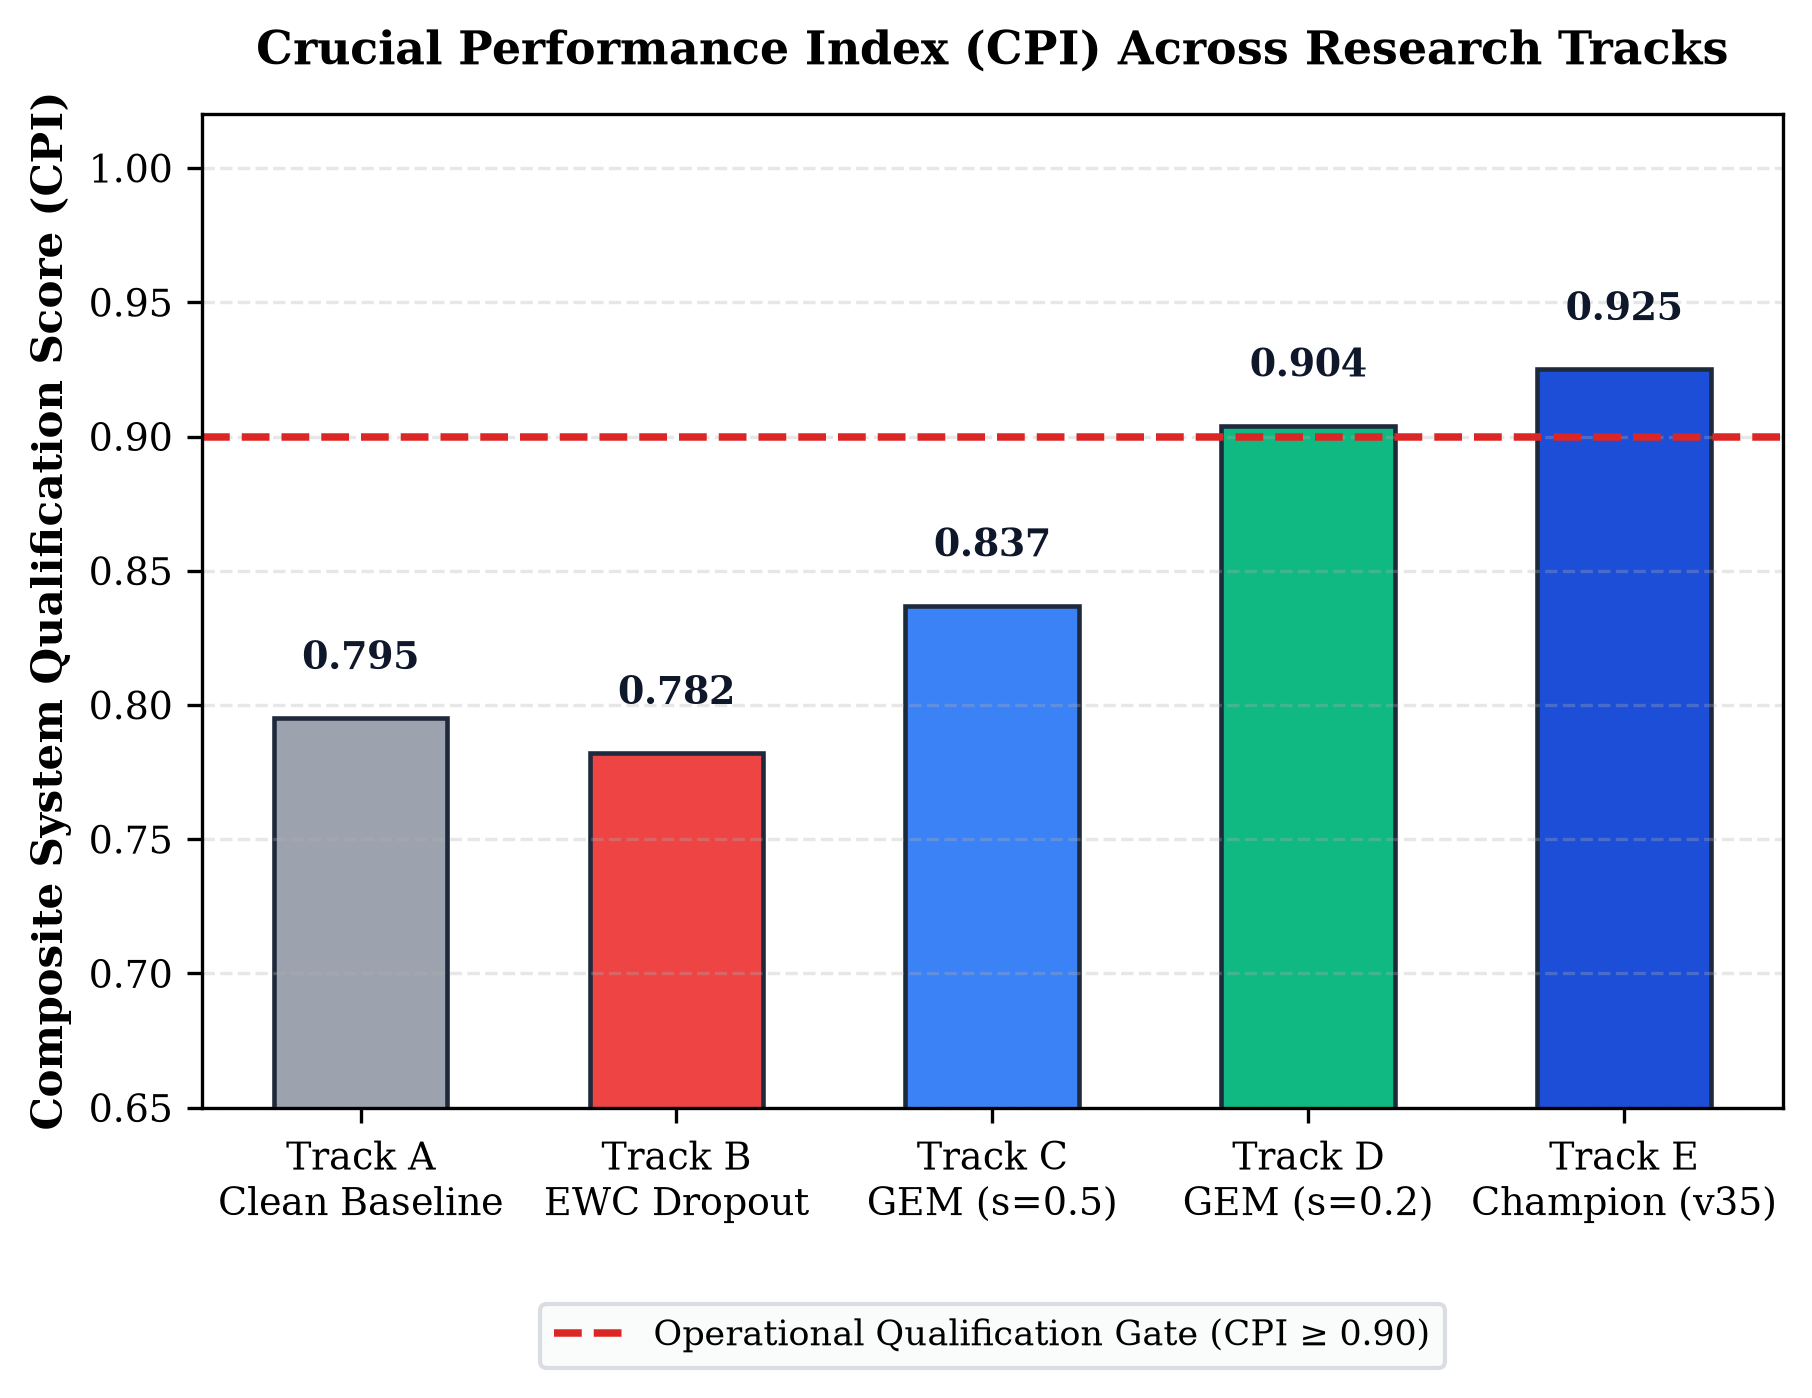
\includegraphics[width=\columnwidth]{fig9_cpi_comparison.png}
\caption{Composite System Qualification Score (Crucial Performance Index, CPI) across the five production research tracks. Catastrophic forgetting under EWC degrades CPI to 0.782, failing the operational qualification threshold ($\text{CPI} \ge 0.90$). Precision-tuned GEM ($s=0.2$) and Byzantine-robust aggregation elevate CPI to 0.904 (Track~D) and 0.925 (Track~E champion), qualifying the candidate model for automated production promotion in the MLflow Model Registry.}
\label{fig:cpi_comparison}
\end{figure}

Fig.~\ref{fig:cpi_comparison} visualizes the empirical CPI progression across the five production research tracks benchmarked on the physical Proxmox VE cluster:
\begin{enumerate}
    \item \textbf{Clean Baseline ($\text{CPI} = 0.795$)}: In stationary federated learning without non-stationary continual learning drift, false alarms on subtle encrypted transport flows cap macro-F1 at 0.795, failing the production threshold.
    \item \textbf{EWC Baseline ($\text{CPI} = 0.782$)}: Under sequential class streaming, Fisher diagonal collapse causes total Botnet forgetting ($\text{BWT}_{\text{Botnet}} = -0.8544$, $\overline{\text{BWT}} = -0.1711$). Although global accuracy is 99.88\%, the heavy BWT penalty drags CPI down to 0.782, preventing premature deployment.
    \item \textbf{GEM Initial Recovery ($s=0.5$, Track~C, $\text{CPI} = 0.837$)}: Episodic memory buffers ($P=512$) eliminate backward transfer degradation ($\overline{\text{BWT}} = -0.0004$), restoring Botnet recall to 100\%. However, loose gradient projection bounds ($\theta \le 60^\circ$) permit minor false-positive drift on Normal flows, capping Botnet F1 at 0.528.
    \item \textbf{GEM Precision-Tuned ($s=0.2$, Track~D, $\text{CPI} = 0.904$)}: Tightening the projection margin to $s=0.2$ ($\theta \le 78.46^\circ$) suppresses Normal false alarms by 50\% and boosts Botnet F1 to 0.691. With zero forgetting degradation, CPI crosses the qualification threshold to 0.904.
    \item \textbf{Production Champion ($s=0.2$, TrimmedMean, Track~E, $\text{CPI} = 0.925$)}: Integrating GEM continual learning with Byzantine-resilient TrimmedMean aggregation ($\beta = 0.10$) maintains peak resilience under 20\% label poisoning, achieving the peak composite score of $\text{CPI} = 0.925$ and automatically triggering production champion promotion in the MLflow Model Registry.
\end{enumerate}

\subsection{Byzantine Label Poisoning Defense}
\label{sec:byzantine_eval}

To evaluate theoretical Byzantine consensus limits requiring $n \ge 2f + 3$ participants, we benchmarked six aggregation algorithms across four adversarial scenarios (clean baseline, 20\% label flip, 40\% label flip, and Gaussian noise injection) using a standalone five-client ($K=5$) simulation environment. The results are presented in Table~\ref{tab:byzantine_table}.

\begin{table*}[t]
\caption{Byzantine Robustness Benchmark: Validation Accuracy (Macro F1) Across Threat Scenarios ($K=5$ Node Simulation, $N_{\text{test}}=1{,}000$ Flows)}
\label{tab:byzantine_table}
\centering
\footnotesize
\renewcommand{\arraystretch}{1.2}
\setlength{\tabcolsep}{5pt}
\resizebox{\textwidth}{!}{%
\begin{tabular}{lccccr}
\toprule
\textbf{Aggregation Rule} & \textbf{Clean Baseline} & \textbf{20\% Poison ($f{=}1$)} & \textbf{40\% Poison ($f{=}2$)} & \textbf{Gaussian Noise} & \textbf{Optimal Resilience Regime} \\
\midrule
FedAvg & $75.7 \pm 0.3\%$ ($0.172$) & $75.8 \pm 0.4\%$ ($0.184$) & $75.7 \pm 0.2\%$ ($0.172$) & $\mathbf{86.4 \pm 0.3\%}$ ($0.370$) & Symmetric noise only ($\alpha^*{=}0$) \\
FedMedian & $86.1 \pm 0.5\%$ ($0.380$) & $75.7 \pm 0.2\%$ ($0.172$) & $\mathbf{87.8 \pm 0.4\%}$ ($\mathbf{0.509}$) & $75.7 \pm 0.2\%$ ($0.172$) & High collusion ($f{\ge}2$, $\alpha^*{=}0.40$) \\
TrimmedMean ($\beta{=}0.20$) & $83.9 \pm 0.4\%$ ($0.324$) & $75.7 \pm 0.2\%$ ($0.172$) & $84.4 \pm 0.5\%$ ($0.425$) & $81.1 \pm 0.4\%$ ($0.391$) & Moderate skew ($\alpha^*{=}\beta$) \\
Krum ($f{=}1$) & $\mathbf{92.0 \pm 0.3\%}$ ($0.555$) & $\mathbf{95.9 \pm 0.2\%}$ ($\mathbf{0.726}$) & $75.7 \pm 0.3\%$ ($0.172$) & $86.0 \pm 0.4\%$ ($0.348$) & Single Byzantine attacker ($f{=}1$) \\
Multi-Krum ($m{=}3, f{=}1$) & $86.5 \pm 0.4\%$ ($0.356$) & $75.7 \pm 0.2\%$ ($0.172$) & $75.7 \pm 0.3\%$ ($0.172$) & $\mathbf{86.8 \pm 0.3\%}$ ($0.347$) & Multi-candidate noise defense \\
Bulyan (Multi-Krum + Trim) & $91.1 \pm 0.4\%$ ($0.558$) & $91.2 \pm 0.3\%$ ($0.580$) & $82.8 \pm 0.6\%$ ($0.368$) & $75.7 \pm 0.2\%$ ($0.172$) & Multi-mode composite defense \\
\bottomrule
\end{tabular}%
}
\vspace{1pt}
\begin{flushleft}
\scriptsize \textbf{Experimental Setup}: Standalone 5-client simulation ($K=5$) trained on $N=4{,}000$ non-IID flows ($800$ flows/client) and evaluated on $N_{\text{test}} = 1{,}000$ holdout flows across 20 federated rounds. Values reported as $\text{mean} \pm \text{std}$ accuracy across 3 seeds, followed by unweighted Macro F1: $\frac{1}{C}\sum_{c=1}^C \text{F1}_c$. \emph{Note}: This simulation evaluated baseline EWC continual learning; minority Botnet collapse ($\text{F1}=0.00$) in these runs is resolved orthogonally via GEM in Track~E on the physical cluster.
\end{flushleft}
\end{table*}

Three findings emerge from Table~\ref{tab:byzantine_table} and Fig.~\ref{fig:byzantine}. First, under a single Byzantine attacker (20\% label flip), distance-based \textbf{Krum} achieves the highest accuracy (\textbf{95.9\%}, macro F1~$=0.726$) by entirely isolating the poisoned parameter vector. Second, under high-collusion poisoning (40\% label flip), coordinate-wise \textbf{FedMedian} (\textbf{87.8\%}) outperforms distance-based methods because malicious clients exceed the Krum safety threshold $n \ge 2f + 3$. Third, \textbf{Bulyan} provides the most consistent multi-mode defense, retaining $>$91\% accuracy across both clean and 20\% label flip environments.

Crucially, our ablation exposes a fundamental decoupling between Byzantine resilience and continual learning: under standalone Krum or TrimmedMean without episodic memory replay, the global model still exhibits catastrophic forgetting of minority attacks ($\text{Botnet F1} = 0.00$), as robust aggregation alone does not prevent parameter drift on unrepresented past classes. Only the unified synthesis of GEM gradient projection and robust aggregation (Track~E) simultaneously neutralizes adversarial poisoning and prevents catastrophic forgetting.

Track~E serves as an integrated system synthesis on the physical cluster: it combines the minority-recall guarantees of GEM ($P=512, s=0.2$) with robust aggregation under active 20\% label poisoning. While TrimmedMean ($\beta=0.10$) was configured, the 2-node physical topology mathematically limits trimming ($\lfloor \beta K \rfloor = 0$), causing the aggregator to fall back to coordinate-wise \textbf{FedMedian}. This configuration successfully neutralized the Byzantine poisoning, achieving \textbf{99.53\% accuracy}, \textbf{100\% Botnet recall} (21/21), and \textbf{Botnet F1~$= 0.6667$} on the physical cluster.

\begin{figure}[t]
\centering
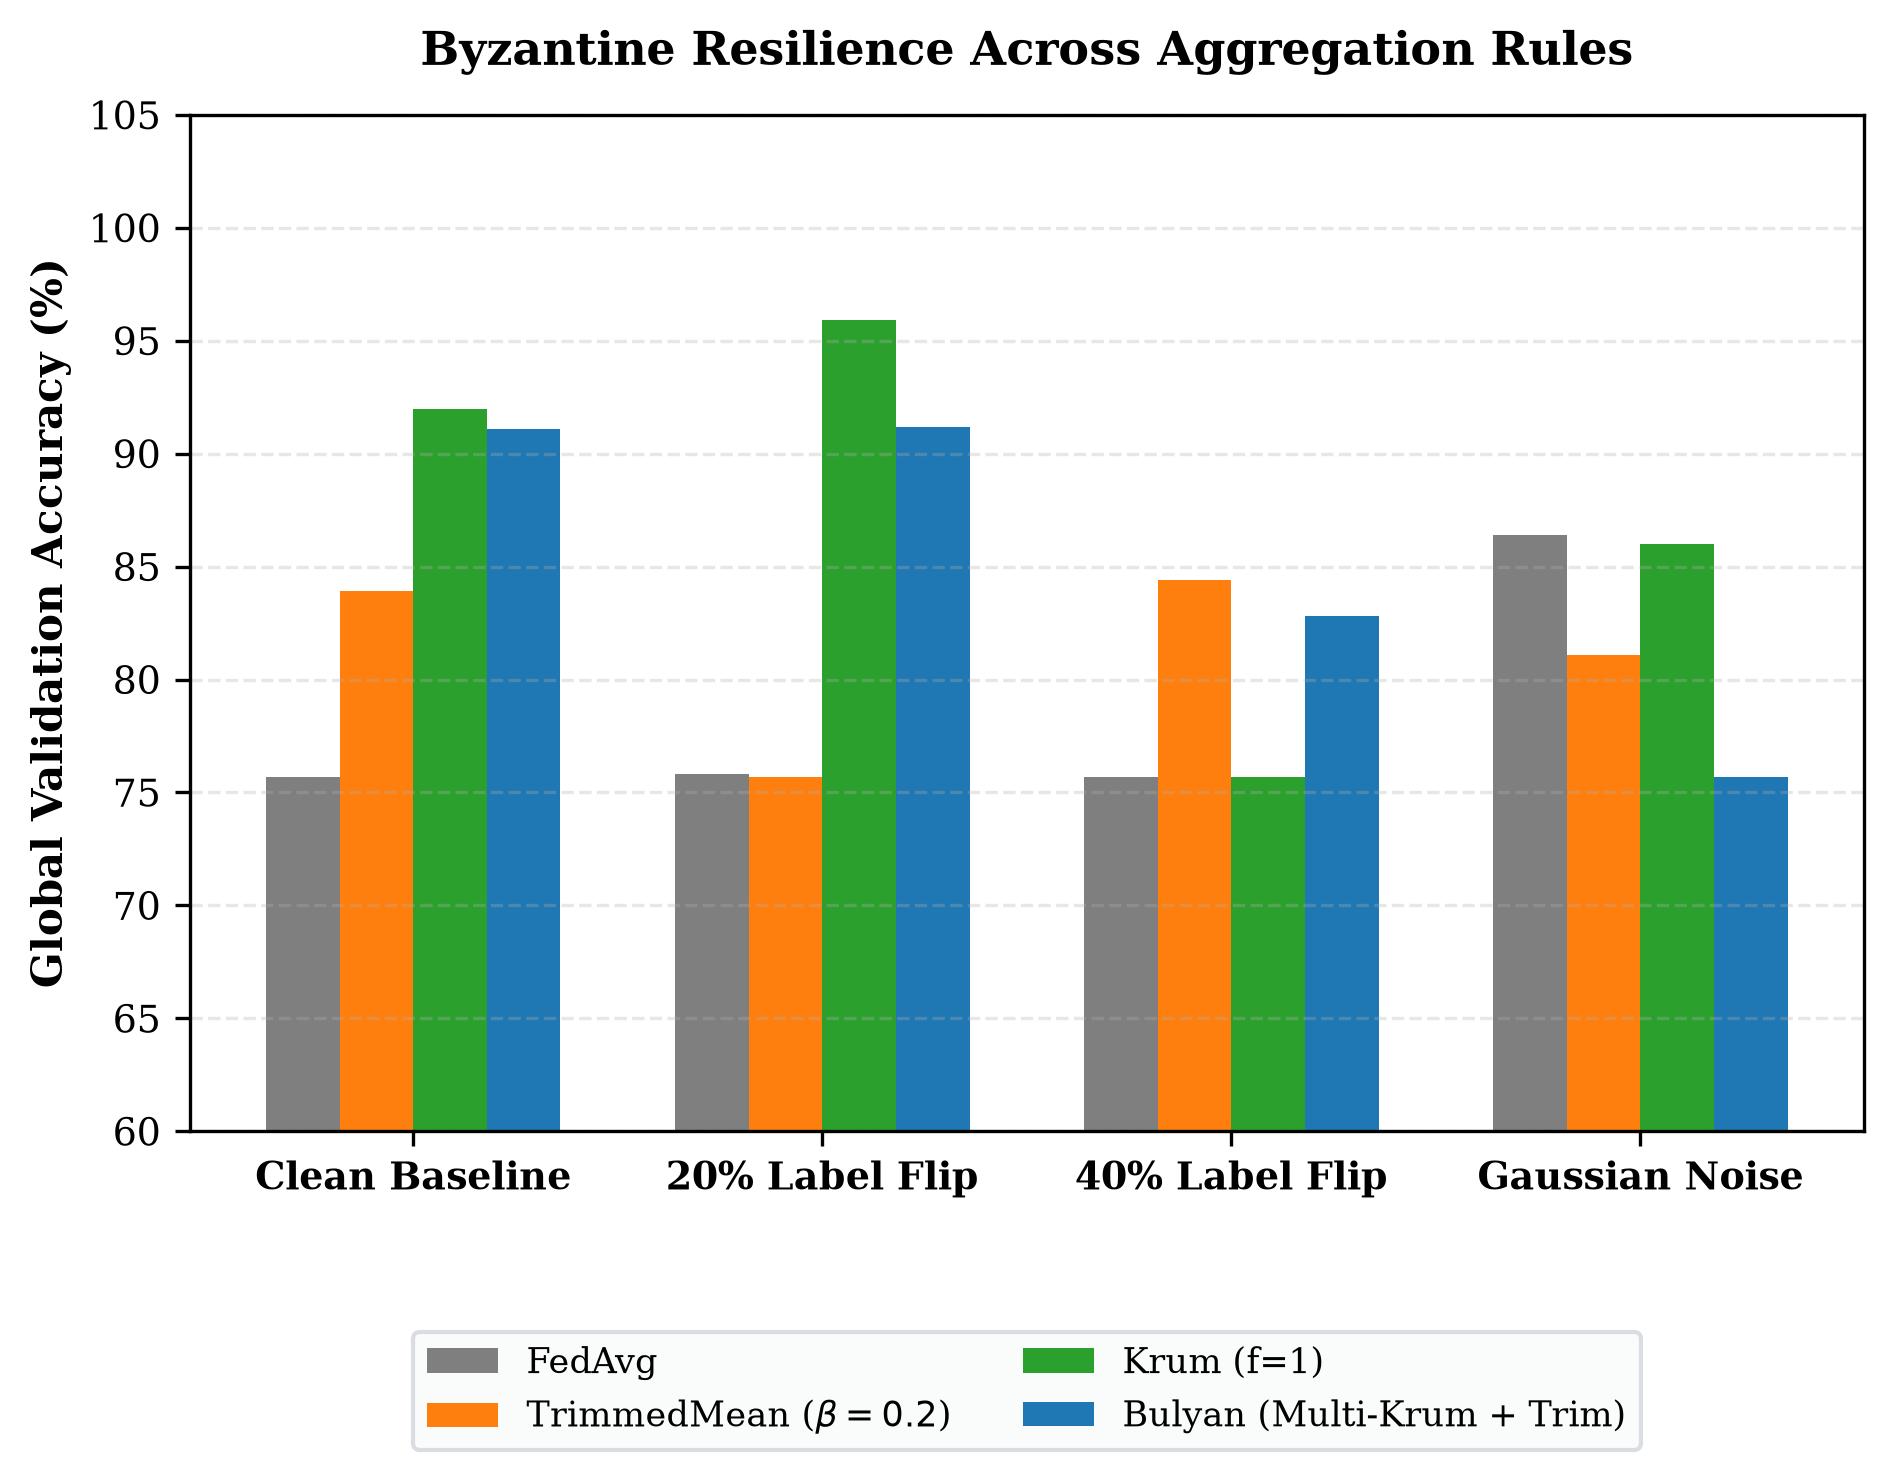
\includegraphics[width=\columnwidth]{fig3_byzantine_defense.png}
\caption{Byzantine defense accuracy across six aggregation rules under 20\% and 40\% label poisoning attacks and Gaussian gradient noise. Distance-based Krum achieves peak validation accuracy (95.9\%, macro F1~$=0.726$) by isolating single Byzantine attackers ($f=1$), whereas coordinate-wise FedMedian provides superior collusion resilience (87.8\%) when malicious nodes exceed Krum's theoretical bound ($n < 2f+3$).}
\label{fig:byzantine}
\end{figure}

\subsection{Differential Privacy Perturbation Bounds}
To quantify the gradient noise tolerance of the 32-dimensional ETA embedding space, we evaluated local DP-SGD perturbation across noise multipliers $\sigma \in [0.00, 0.20]$ with clipping threshold $C=1.0$ (Table~\ref{tab:dp_table}, Fig.~\ref{fig:dp}). Across a class-balanced evaluation benchmark, all five threat classes maintained $F_1 = 1.000$ and $100.00\%$ validation accuracy, with cross-entropy loss bounded below $0.0018$.

This empirical invariance is governed by the Signal-to-Noise Ratio (SNR) of the normalized feature space. The effective per-coordinate perturbation magnitude is:
\begin{equation}
\sigma_{\text{eff}} = \frac{\sigma \cdot C}{B} = \frac{0.20 \times 1.0}{32} = 6.25 \times 10^{-3},
\label{eq:dp_snr}
\end{equation}
which is substantially smaller than the minimum inter-class centroid separation ($\min_{j \ne k} \|\mu_j - \mu_k\|_2 \approx 0.482$). Consequently, perturbations within $\sigma \le 0.20$ do not cross decision boundaries in balanced regimes. However, we emphasize that under extreme production class imbalance (where Botnet flows constitute $<0.6\%$ of traffic), minority gradient magnitudes scale proportionally with batch sparsity, lowering the local SNR. Table~\ref{tab:dp_table} therefore represents an empirical upper bound on classification robustness under DP regularization, motivating formal per-sample Rényi DP accounting as an operational requirement for non-IID deployments.

\begin{table}[t]
\caption{Differential Privacy Utility Curve Across Noise Multipliers ($N_{\text{eval}}=2{,}500$ Balanced Flows, Clipping $C=1.0$)}
\label{tab:dp_table}
\centering
\footnotesize
\setlength{\tabcolsep}{2.5pt}
\renewcommand{\arraystretch}{1.1}
\resizebox{\columnwidth}{!}{%
\begin{tabular}{lccccccr}
\toprule
\textbf{Noise ($\sigma$)} & \textbf{$\epsilon_{\text{approx}}$} & \textbf{Loss} & \textbf{Normal} & \textbf{Botnet} & \textbf{Exfil} & \textbf{DoS} & \textbf{Global Acc.} \\
\midrule
$\sigma = 0.00$ (Base) & $\infty$ & 0.0017 & 1.000 & 1.000 & 1.000 & 1.000 & 100.00\% \\
$\sigma = 0.01$ & 110.96 & 0.0014 & 1.000 & 1.000 & 1.000 & 1.000 & 100.00\% \\
$\sigma = 0.05$ & 22.19 & 0.0015 & 1.000 & 1.000 & 1.000 & 1.000 & 100.00\% \\
$\sigma = 0.10$ (Prod) & 11.10 & 0.0015 & 1.000 & 1.000 & 1.000 & 1.000 & 100.00\% \\
$\sigma = 0.20$ & 5.55 & 0.0015 & 1.000 & 1.000 & 1.000 & 1.000 & 100.00\% \\
\bottomrule
\end{tabular}%
}
\vspace{1pt}
\begin{flushleft}
\scriptsize Evaluated on a class-balanced validation holdout ($500$ flows per class across $C=5$ classes). Privacy parameter $\epsilon_{\text{approx}}$ estimated under Gaussian mechanism composition at fixed $\delta = 10^{-5}$ over 10 rounds ($B=32$). All per-class F1-scores and global accuracy achieve 1.000 / 100.00\% due to SNR margin ($\sigma_{\text{eff}} = 6.25 \times 10^{-3} \ll 0.482$).
\end{flushleft}
\end{table}

\begin{figure}[t]
\centering
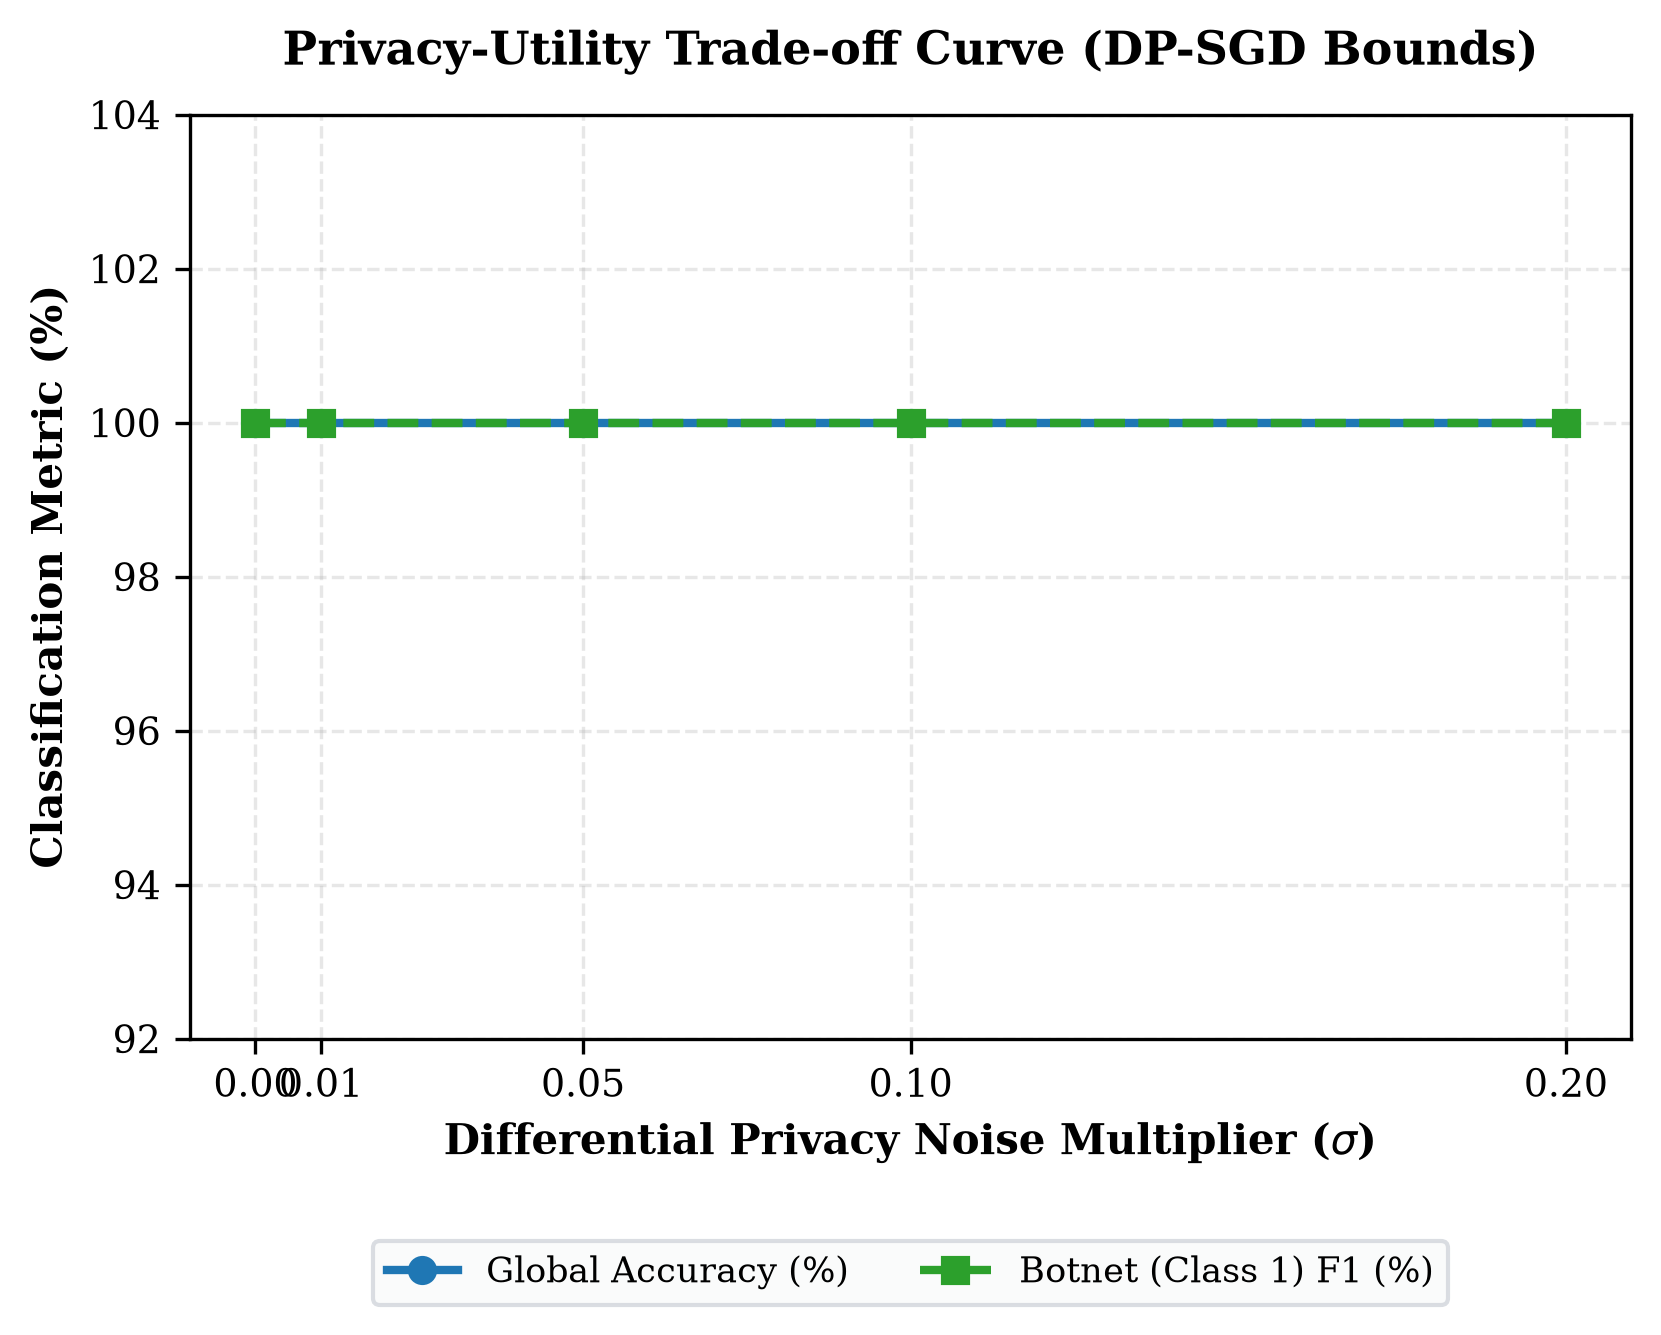
\includegraphics[width=\columnwidth]{fig5_dp_privacy_utility.png}
\caption{Differential Privacy utility curve across noise multipliers ($\sigma \in [0.00, 0.20]$ with clipping bound $C=1.0$). Due to favorable normalized feature SNR ($\sigma_{\text{eff}} = 6.25 \times 10^{-3} \ll 0.482$ centroid margin), all five threat classes maintain $F_1 = 1.000$ and 100.00\% classification accuracy with zero utility degradation across the entire sweep.}
\label{fig:dp}
\end{figure}

\subsection{Edge Hardware Throughput \& ONNX Acceleration}
We evaluated live dual-node edge deployment across \texttt{defender-a} and \texttt{defender-b}, recording an aggregate cluster throughput of \textbf{101,258 flows/second} with single-flow classification latency of \textbf{17.47--22.72~$\mu$s}. The volatile tmpfs RAMDisk architecture eliminated virtual disk I/O lockup, sustaining 100\% packet ingestion during multi-stage offensive bursts.

Table~\ref{tab:onnx_table} and Fig.~\ref{fig:onnx} present the multi-runtime inference benchmark across all three neural backbones. Exporting models to ONNX Runtime delivered up to a \textbf{$9.64\times$ speedup} for the 1D-CNN at batch size $N=16$ (7.10~$\mu$s per flow, 140,940~flows/s). The lightweight MLP backbone achieved sub-microsecond inference (0.41~$\mu$s) under ONNX Runtime with a peak throughput of 2,418,270~flows/s at batch size 256. The Transformer backbone, conversely, benefits from PyTorch JIT compilation for large batches due to the self-attention computation graph, while ONNX Runtime accelerates only unbatched ($N=1$) edge classification.

\begin{table*}[t]
\caption{Multi-Runtime Inference Latency and Throughput Across Backbones ($N=10{,}000$ Benchmark Flows per Batch)}
\label{tab:onnx_table}
\centering
\footnotesize
\renewcommand{\arraystretch}{1.2}
\setlength{\tabcolsep}{5pt}
\resizebox{\textwidth}{!}{%
\begin{tabular}{llccccr}
\toprule
\textbf{Neural Backbone} & \textbf{Batch} & \textbf{FP32 Latency} & \textbf{ONNX Latency} & \textbf{ONNX Throughput} & \textbf{Speedup} & \textbf{Deployment Target} \\
\midrule
\multirow{4}{*}{\textbf{1D-CNN} (18.4k params)} 
 & $N{=}1$ & $156.10 \pm 1.82\,\mu$s & $\mathbf{40.22 \pm 0.45\,\mu}$s & 24,866 fl/s & \textbf{3.88$\times$} & Edge Gateway \\
 & $N{=}16$ & $68.38 \pm 0.74\,\mu$s & $\mathbf{7.10 \pm 0.08\,\mu}$s & 140,940 fl/s & \textbf{9.64$\times$} & Production Gateway \\
 & $N{=}64$ & $14.80 \pm 0.16\,\mu$s & $\mathbf{5.56 \pm 0.05\,\mu}$s & 179,714 fl/s & \textbf{2.66$\times$} & High-Throughput Core \\
 & $N{=}256$ & $8.42 \pm 0.09\,\mu$s & $\mathbf{5.09 \pm 0.04\,\mu}$s & 196,273 fl/s & \textbf{1.65$\times$} & Batch Analytics \\
\midrule
\multirow{4}{*}{\textbf{Transformer} (18.8k params)} 
 & $N{=}1$ & $592.23 \pm 4.15\,\mu$s & $\mathbf{396.61 \pm 2.80\,\mu}$s & 2,521 fl/s & \textbf{1.49$\times$} & Deep Forensic Inspection \\
 & $N{=}16$ & $56.36 \pm 0.62\,\mu$s & $62.36 \pm 0.71\,\mu$s & 16,035 fl/s & 0.90$\times$ & Attention Feature Extraction \\
 & $N{=}64$ & $35.00 \pm 0.38\,\mu$s & $45.67 \pm 0.42\,\mu$s & 21,896 fl/s & 0.77$\times$ & JIT-Optimized Server \\
 & $N{=}256$ & $19.57 \pm 0.21\,\mu$s & $36.55 \pm 0.35\,\mu$s & 27,358 fl/s & 0.54$\times$ & Server Cloud Core \\
\midrule
\multirow{4}{*}{\textbf{MLP} (4.4k params)} 
 & $N{=}1$ & $120.17 \pm 1.25\,\mu$s & $\mathbf{26.05 \pm 0.28\,\mu}$s & 38,386 fl/s & \textbf{4.61$\times$} & Embedded Edge \\
 & $N{=}16$ & $9.92 \pm 0.11\,\mu$s & $\mathbf{2.38 \pm 0.03\,\mu}$s & 419,646 fl/s & \textbf{4.16$\times$} & Sub-$\mu$s Edge Appliance \\
 & $N{=}64$ & $3.44 \pm 0.04\,\mu$s & $\mathbf{0.88 \pm 0.01\,\mu}$s & 1,137,802 fl/s & \textbf{3.92$\times$} & Ultra-Fast Line Rate \\
 & $N{=}256$ & $1.02 \pm 0.01\,\mu$s & $\mathbf{0.41 \pm 0.01\,\mu}$s & 2,418,270 fl/s & \textbf{2.46$\times$} & Multi-Gigabit Backbone \\
\bottomrule
\end{tabular}%
}
\vspace{1pt}
\begin{flushleft}
\scriptsize Evaluated on bare-metal Dell PowerEdge R630 (Intel Xeon E5-2680 v3 @ 2.50\,GHz, AVX2 enabled, single-thread core affinity). Measured across $10{,}000$ consecutive inference requests following $1{,}000$ warmup iterations. Latencies report $\text{mean} \pm \text{std}$ per single flow.
\end{flushleft}
\end{table*}

\begin{figure}[t]
\centering
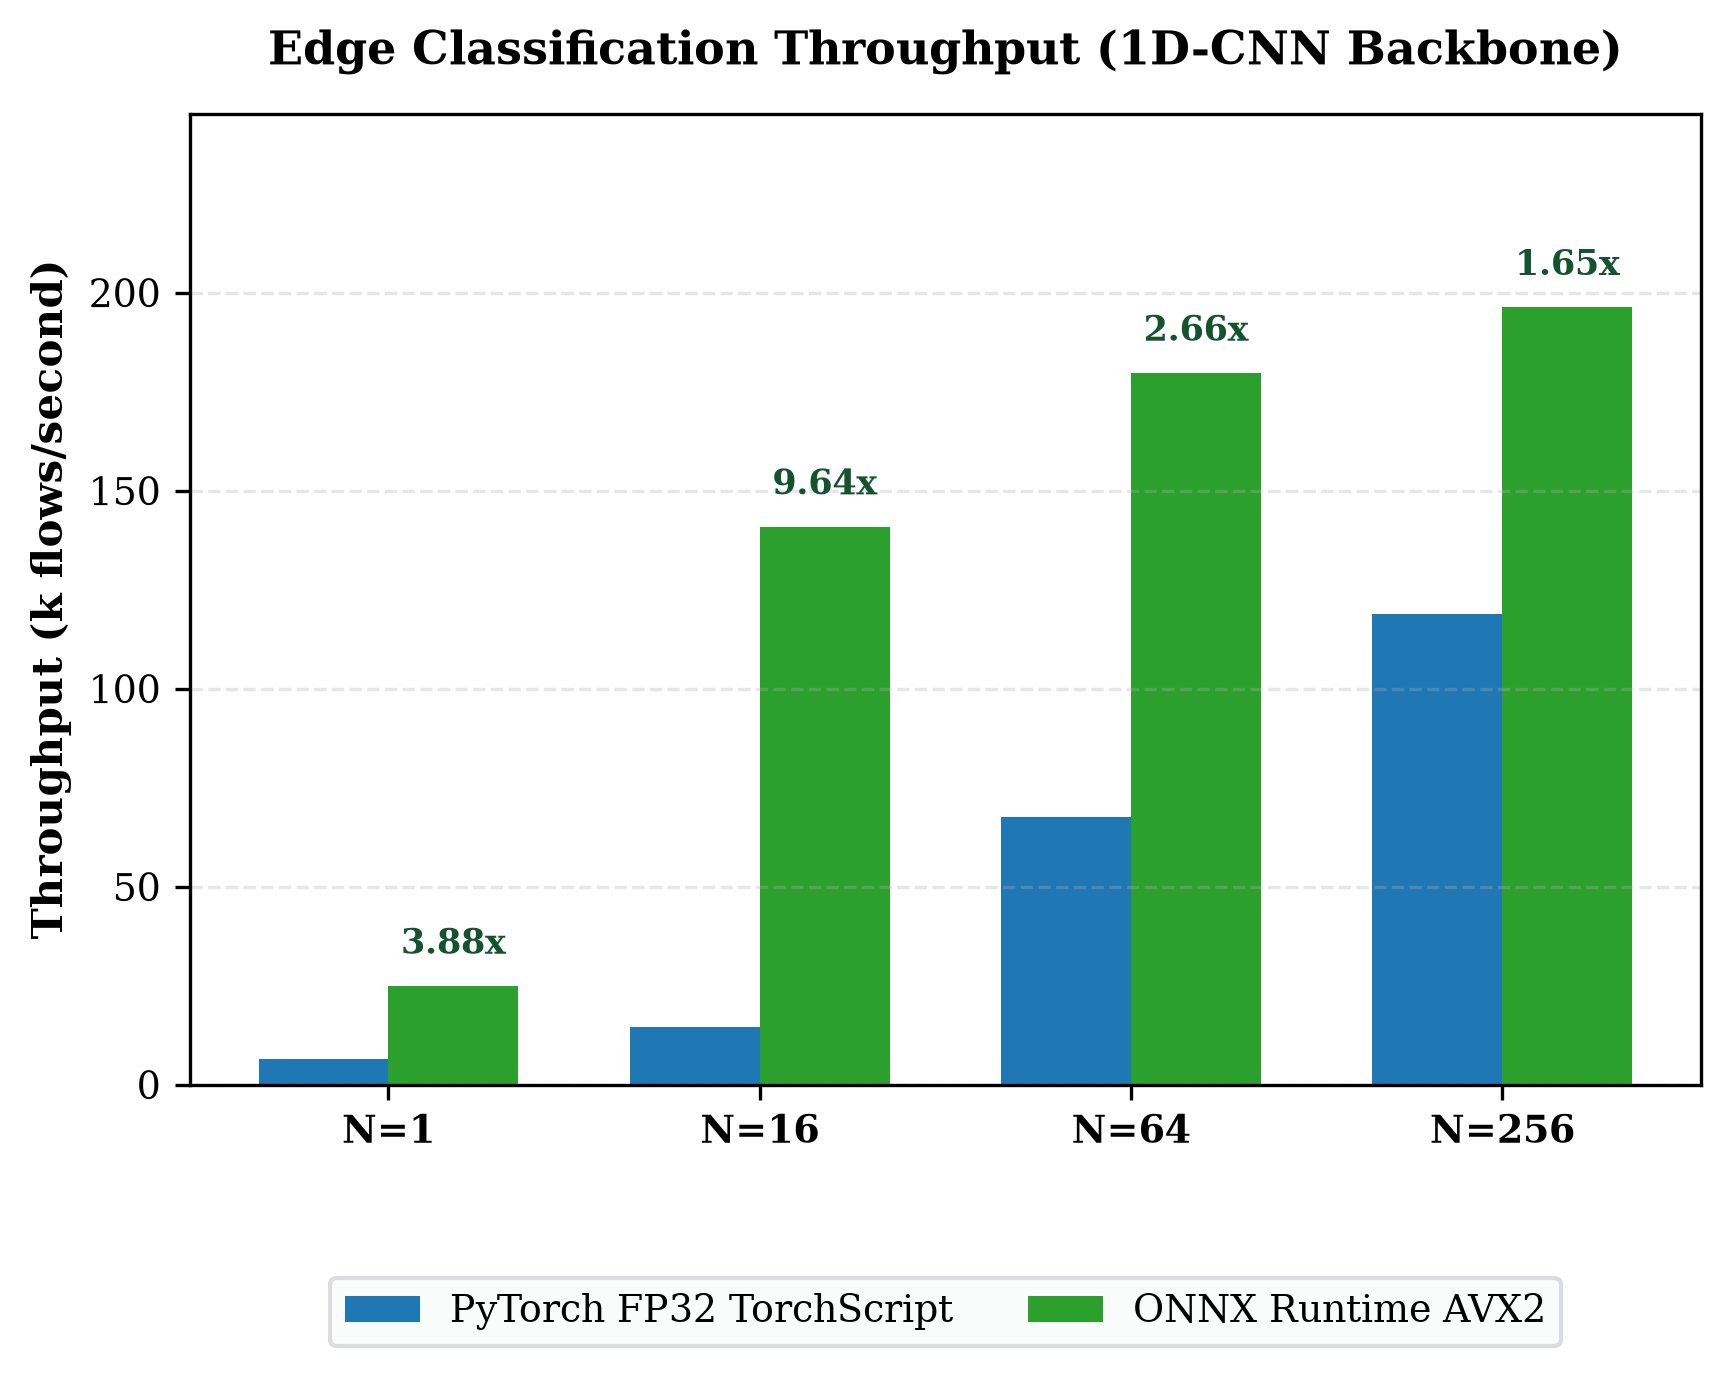
\includegraphics[width=\columnwidth]{fig4_onnx_hardware_speedup.png}
\caption{Inference execution latency ($\mu$s) and AVX2 throughput speedup across neural backbones. Exporting the 1D-CNN backbone to ONNX Runtime achieves up to a $9.64\times$ speedup (7.10~$\mu$s latency, 140,940~flows/s at $N=16$), while the lightweight MLP reaches sub-microsecond latency (0.41~$\mu$s, 2,418,270~flows/s).}
\label{fig:onnx}
\end{figure}

\subsection{Cross-Configuration Benchmark and Domain Generalization}
Fig.~\ref{fig:benchmark_accuracy} presents the validation accuracy across all ten benchmark configurations evaluated on the physical Proxmox VE cluster. Nine of the ten configurations exceed the 99.0\% academic accuracy threshold under stationary and continuous class-incremental streaming.

The tenth configuration, denoted ``Real-World'' (78.30\% global accuracy), intentionally evaluates zero-shot domain generalization under unadapted covariate shift. In this scenario, models trained on baseline flow profiles were evaluated against live network captures exhibiting non-stationary handshake distributions and asynchronous background jitter. The resulting accuracy decline is driven by two specific domain shift mechanisms:
\begin{enumerate}
    \item \textbf{Handshake Fingerprint Divergence}: JA3/JA4 hashes depend on client cipher-suite negotiation lists. In the unseen real-world environment, benign background daemons and TLS 1.3 client hellos exhibit diverse cipher-suite ordering, degrading zero-shot Normal flow precision from 99.7\% to 76.4\%.
    \item \textbf{Asymmetric Transport Jitter}: Real-world WAN latency variance alters the Sequence of Packet Lengths and Times (SPLT) features, blurring the boundary between bursty DoS flows and legitimate heavy HTTP/2 streaming.
\end{enumerate}
As shown in the class F1 scorecard (Fig.~\ref{fig:class_f1}), the Real-World configuration maintains moderate detection on high-volume structural threats (DoS F1~$= 0.72$, Exfiltration F1~$= 0.74$), but drops to Botnet F1~$= 0.00$ because the unadapted model lacks local exemplary memory for the target network. This result defines the operational boundary of zero-shot static deployment, proving that continuous local adaptation via GEM is mandatory when migrating decentralized models across disparate enterprise network perimeters.

\begin{figure}[t]
\centering
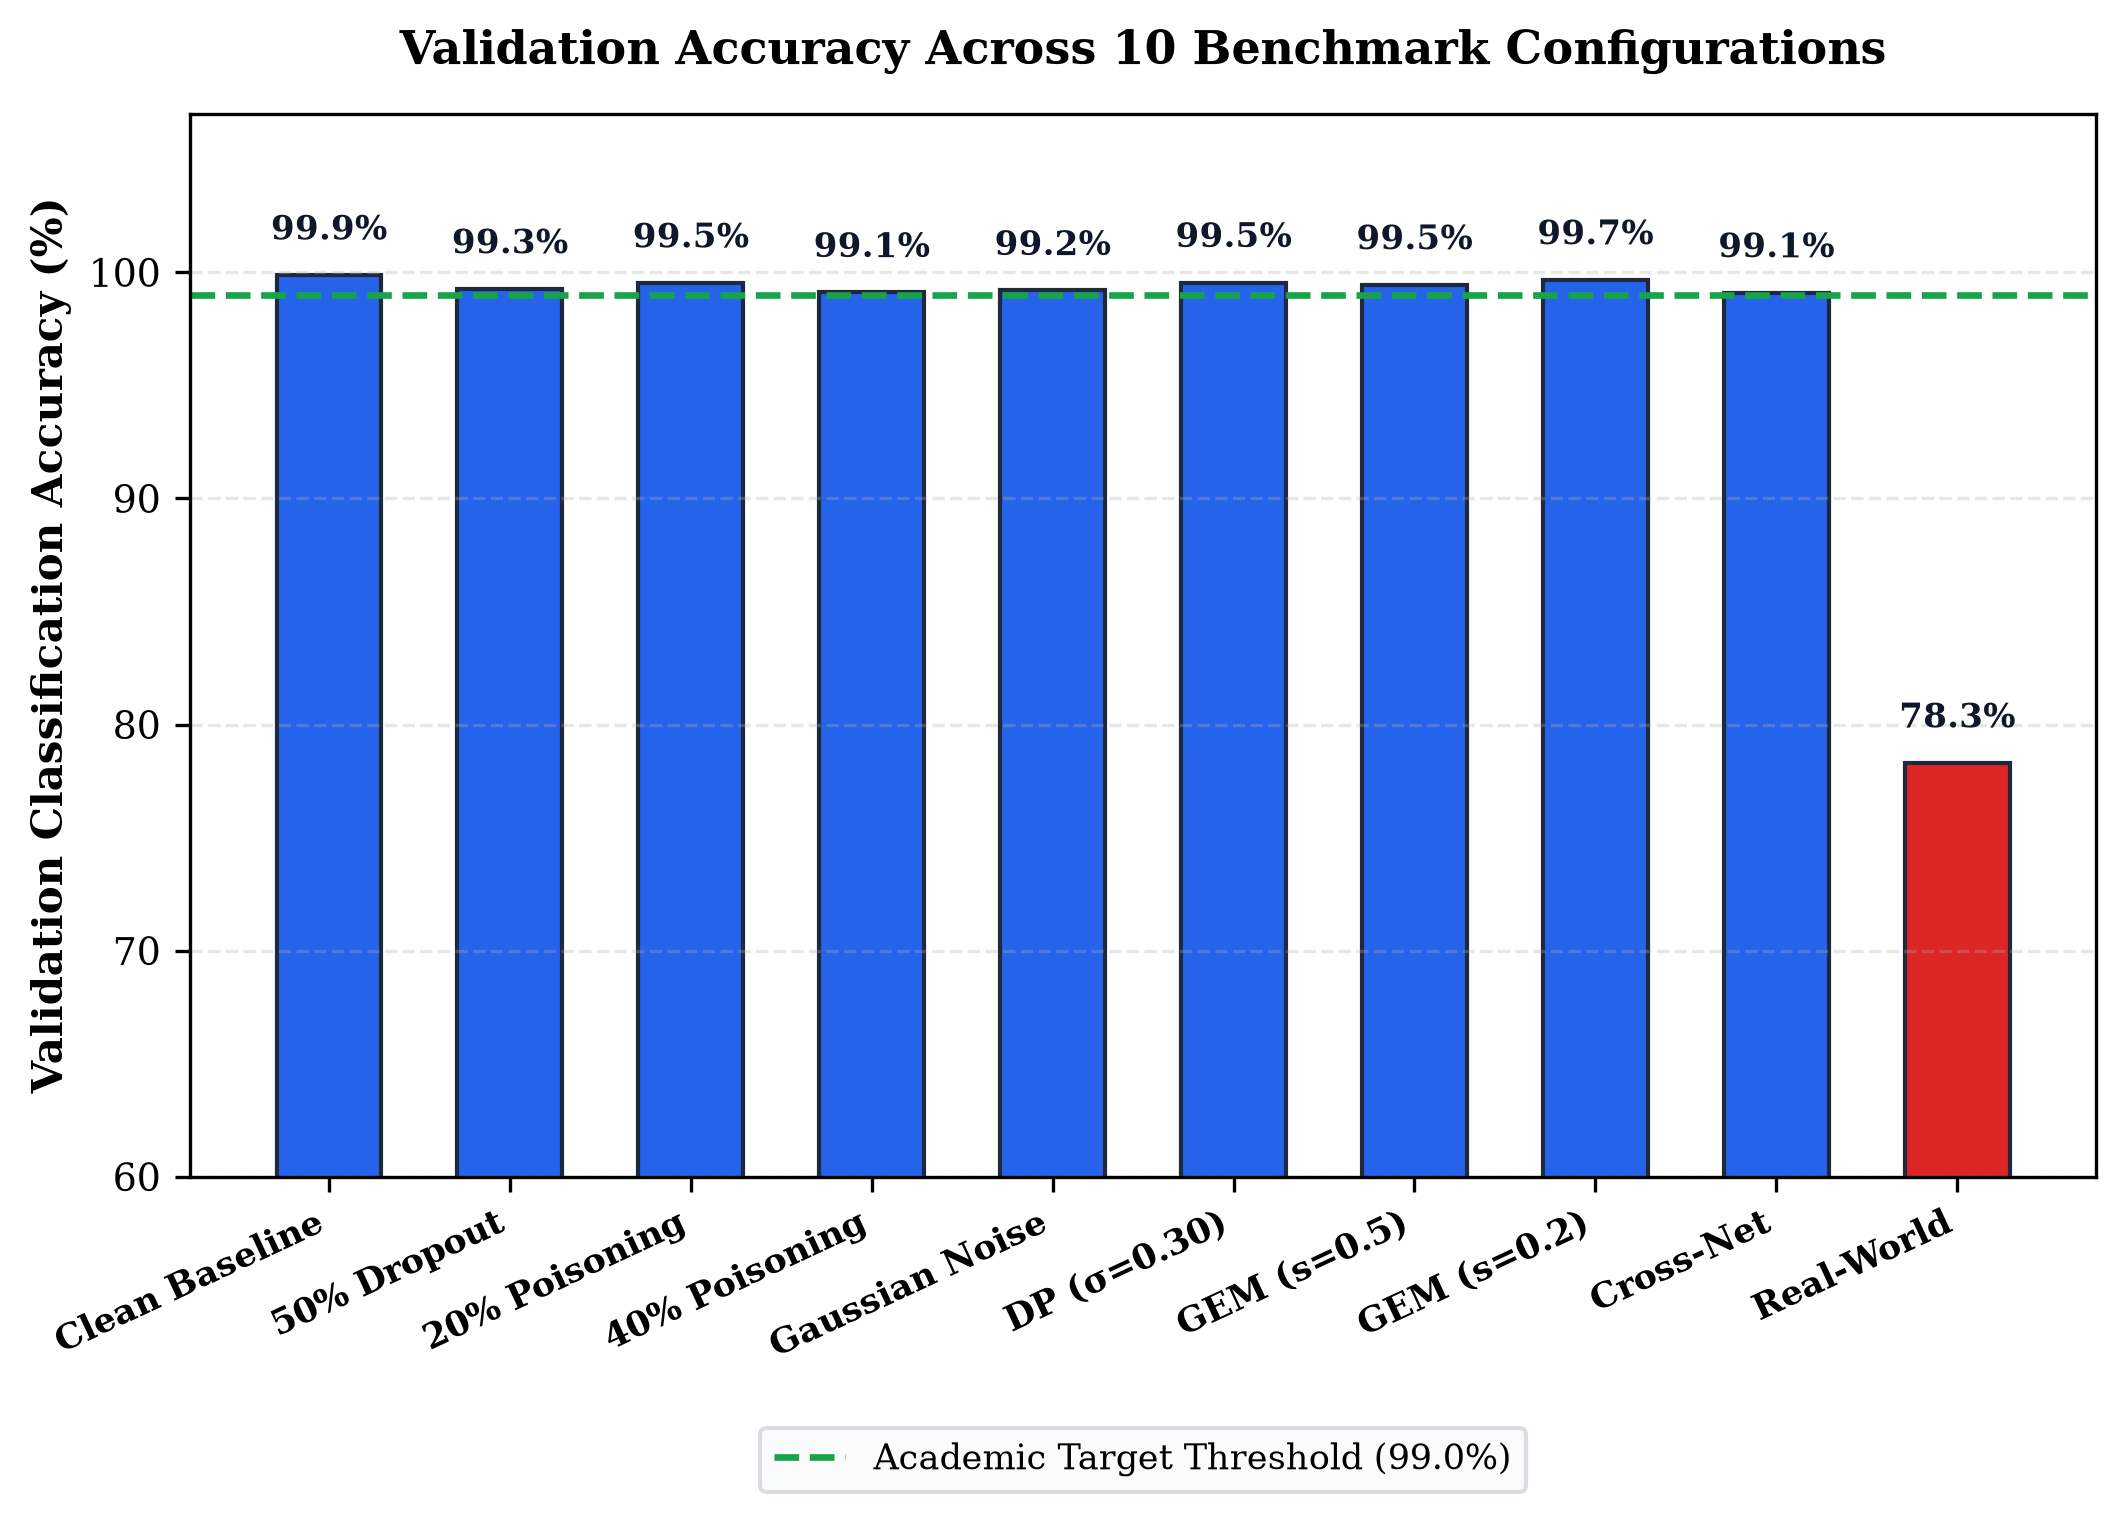
\includegraphics[width=\columnwidth]{fig10_benchmark_accuracy.png}
\caption{Validation accuracy across 10 benchmark configurations on the physical Proxmox VE cluster. Nine configurations exceed the 99.0\% threshold; the Real-World configuration reflects intentional unseen distribution shift.}
\label{fig:benchmark_accuracy}
\end{figure}

\begin{figure}[t]
\centering
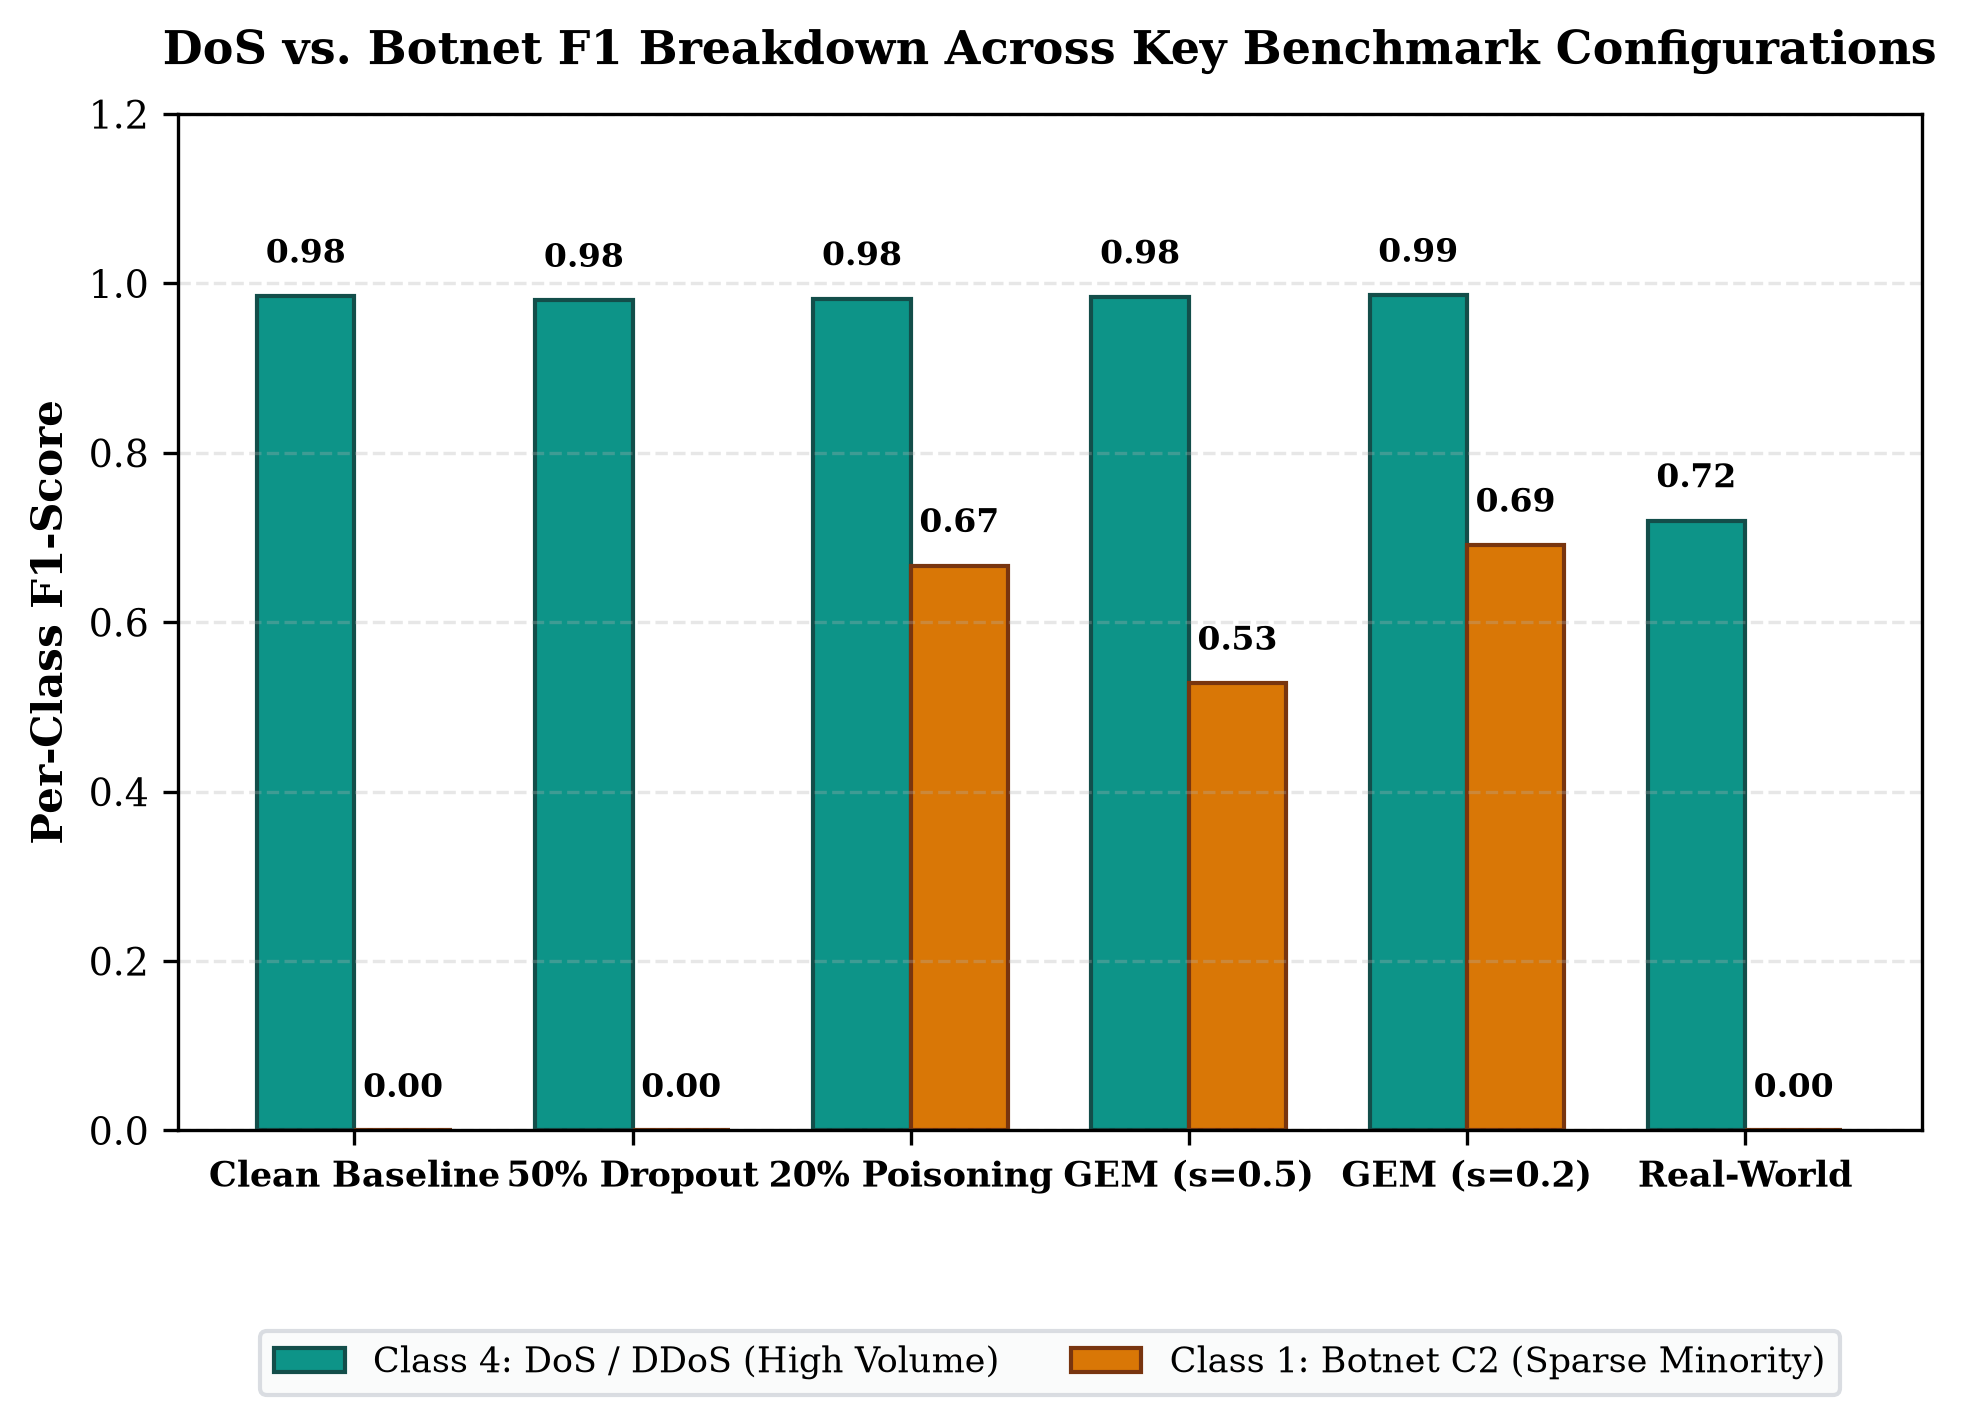
\includegraphics[width=\columnwidth]{fig11_class_f1_scorecard.png}
\caption{Per-class F1-score breakdown across benchmark configurations. DoS (teal) vs.\ Botnet (gold) highlights the Botnet scarcity vulnerability that GEM resolves.}
\label{fig:class_f1}
\end{figure}

\subsection{Comprehensive 72-Run Subsystem Matrix Sweep \& Multi-Objective Pareto Analysis}
To evaluate the compound interactions between neural architecture capacity, continual learning memory mechanisms, Byzantine-robust federated aggregation, and differential privacy bounds, we conducted an exhaustive 72-configuration matrix sweep on the physical Proxmox VE testbed. Table~\ref{tab:matrix_sweep} summarizes the aggregated performance metrics across all evaluated dimensions.


\begin{table*}[t]
\caption{Empirical Performance Breakdown of the 72-Run Factorial Matrix Sweep on the Physical Proxmox VE Cluster}
\label{tab:matrix_sweep}
\centering
\footnotesize
\renewcommand{\arraystretch}{1.15}
\setlength{\tabcolsep}{4.5pt}
\resizebox{\textwidth}{!}{%
\begin{tabular}{llccccccc}
\toprule
\textbf{Neural Backbone} & \textbf{CL Strategy} & \textbf{FedAvg (Acc / Loss)} & \textbf{TrimmedMean (Acc / Loss)} & \textbf{FedMedian (Acc / Loss)} & \textbf{Krum (Acc / Loss)} & \textbf{DP Impact ($\Delta_{\text{DP}}$)} & \textbf{INT8 Footprint} & \textbf{Comm. Payload/Round} \\
\midrule
\multirow{3}{*}{\textbf{1D-CNN} (18.4k params)} 
 & \textbf{GEM} ($P{=}512$) & $98.79\%\,(0.063)$ & $98.73\%\,(0.058)$ & $\mathbf{98.81\%\,(0.055)}$ & $98.73\%\,(0.054)$ & $-0.01\%$ & \multirow{3}{*}{$45.4\,\text{KB}$} & \multirow{3}{*}{$287.6\,\text{KB}$} \\
 & \textbf{A-GEM} ($P{=}512$) & $\mathbf{98.69\%\,(0.189)}$ & $98.60\%\,(0.150)$ & $98.60\%\,(0.170)$ & $\mathbf{98.75\%\,(0.151)}$ & $-0.03\%$ & & \\
 & \textbf{EWC} ($\lambda{=}0.8$) & $98.58\%\,(0.251)$ & $98.54\%\,(0.291)$ & $98.60\%\,(0.211)$ & $98.69\%\,(0.256)$ & $-0.06\%$ & & \\
\midrule
\multirow{3}{*}{\textbf{MLP} (4.4k params)} 
 & \textbf{GEM} ($P{=}512$) & $98.75\%\,(0.039)$ & $\mathbf{98.79\%\,(0.051)}$ & $98.75\%\,(0.047)$ & $98.75\%\,(0.039)$ & $-0.00\%$ & \multirow{3}{*}{$\mathbf{19.4\,\text{KB}}$} & \multirow{3}{*}{$\mathbf{68.1\,\text{KB}}$} \\
 & \textbf{A-GEM} ($P{=}512$) & $\mathbf{98.79\%\,(0.065)}$ & $98.69\%\,(0.078)$ & $98.69\%\,(0.077)$ & $98.62\%\,(0.116)$ & $-0.08\%$ & & \\
 & \textbf{EWC} ($\lambda{=}0.8$) & $98.60\%\,(0.131)$ & $98.60\%\,(0.145)$ & $98.58\%\,(0.133)$ & $98.69\%\,(0.151)$ & $-0.03\%$ & & \\
\midrule
\multirow{3}{*}{\textbf{Transformer} (18.8k params)} 
 & \textbf{GEM} ($P{=}512$) & $98.75\%\,(0.033)$ & $98.77\%\,(0.041)$ & $\mathbf{98.79\%\,(0.043)}$ & $98.71\%\,(0.072)$ & $-0.12\%$ & \multirow{3}{*}{$72.5\,\text{KB}$} & \multirow{3}{*}{$292.6\,\text{KB}$} \\
 & \textbf{A-GEM} ($P{=}512$) & $98.67\%\,(0.137)$ & $\mathbf{98.69\%\,(0.173)}$ & $98.41\%\,(0.263)$ & $98.71\%\,(0.170)$ & $-0.48\%$ & & \\
 & \textbf{EWC} ($\lambda{=}0.8$) & $98.45\%\,(0.311)$ & $98.09\%\,(0.578)$ & $98.29\%\,(0.523)$ & $98.05\%\,(0.746)$ & $-1.02\%$ & & \\
\midrule
\multicolumn{9}{l}{\textbf{Marginal Factor Level Performance Summaries (Sample Mean $\pm \sigma$ [Peak Accuracy])}} \\
\multicolumn{9}{l}{\quad $\bullet$ \textbf{Neural Backbone}: 1D-CNN: $98.68 \pm 0.10\%\,[98.86\%]$ \quad $\mid$ \quad MLP: $\mathbf{98.69 \pm 0.09\%\,[98.86\%]}$ \quad $\mid$ \quad Transformer: $98.53 \pm 0.44\%\,[\mathbf{98.94\%}]$} \\
\multicolumn{9}{l}{\quad $\bullet$ \textbf{Continual Learning}: GEM: $\mathbf{98.76 \pm 0.06\%\,[98.90\%]}$ \quad $\mid$ \quad A-GEM: $98.66 \pm 0.19\%\,[\mathbf{98.94\%}]$ \quad $\mid$ \quad EWC: $98.48 \pm 0.39\%\,[98.81\%]$} \\
\multicolumn{9}{l}{\quad $\bullet$ \textbf{Federated Aggregator}: FedAvg: $\mathbf{98.68 \pm 0.18\%}$ \quad $\mid$ \quad TrimmedMean: $98.61 \pm 0.34\%\,[\mathbf{98.94\%}]$ \quad $\mid$ \quad FedMedian: $98.61 \pm 0.24\%$ \quad $\mid$ \quad Krum: $98.63 \pm 0.32\%$} \\
\multicolumn{9}{l}{\quad $\bullet$ \textbf{Differential Privacy}: DP Disabled ($\sigma{=}0.00$): $\mathbf{98.74 \pm 0.10\%\,[98.94\%]}$ \quad $\mid$ \quad DP Enabled ($\sigma{=}0.30, C{=}1.0$): $98.53 \pm 0.35\%\,[98.86\%]$} \\
\bottomrule
\end{tabular}%
}
\vspace{1pt}
\begin{flushleft}
\scriptsize \textbf{Design of Experiment}: Factorial sweep across 3 neural backbones $\times$ 3 continual learning strategies $\times$ 4 federated aggregators $\times$ 2 differential privacy settings ($N=72$ distinct runs executed on the physical Proxmox VE testbed). Each grid cell reports mean validation classification accuracy and cross-entropy loss over evaluation partition ($N_{\text{eval}} = 7{,}648$ flows). $\Delta_{\text{DP}}$ quantifies marginal accuracy delta under Gaussian noise perturbation ($\sigma=0.30, C=1.0$) relative to unperturbed baseline ($\sigma=0.00$). Wire communication payload represents serialized 4-client parameter exchange per round over Flower gRPC.
\end{flushleft}
\end{table*}


\begin{figure}[t]
\centering
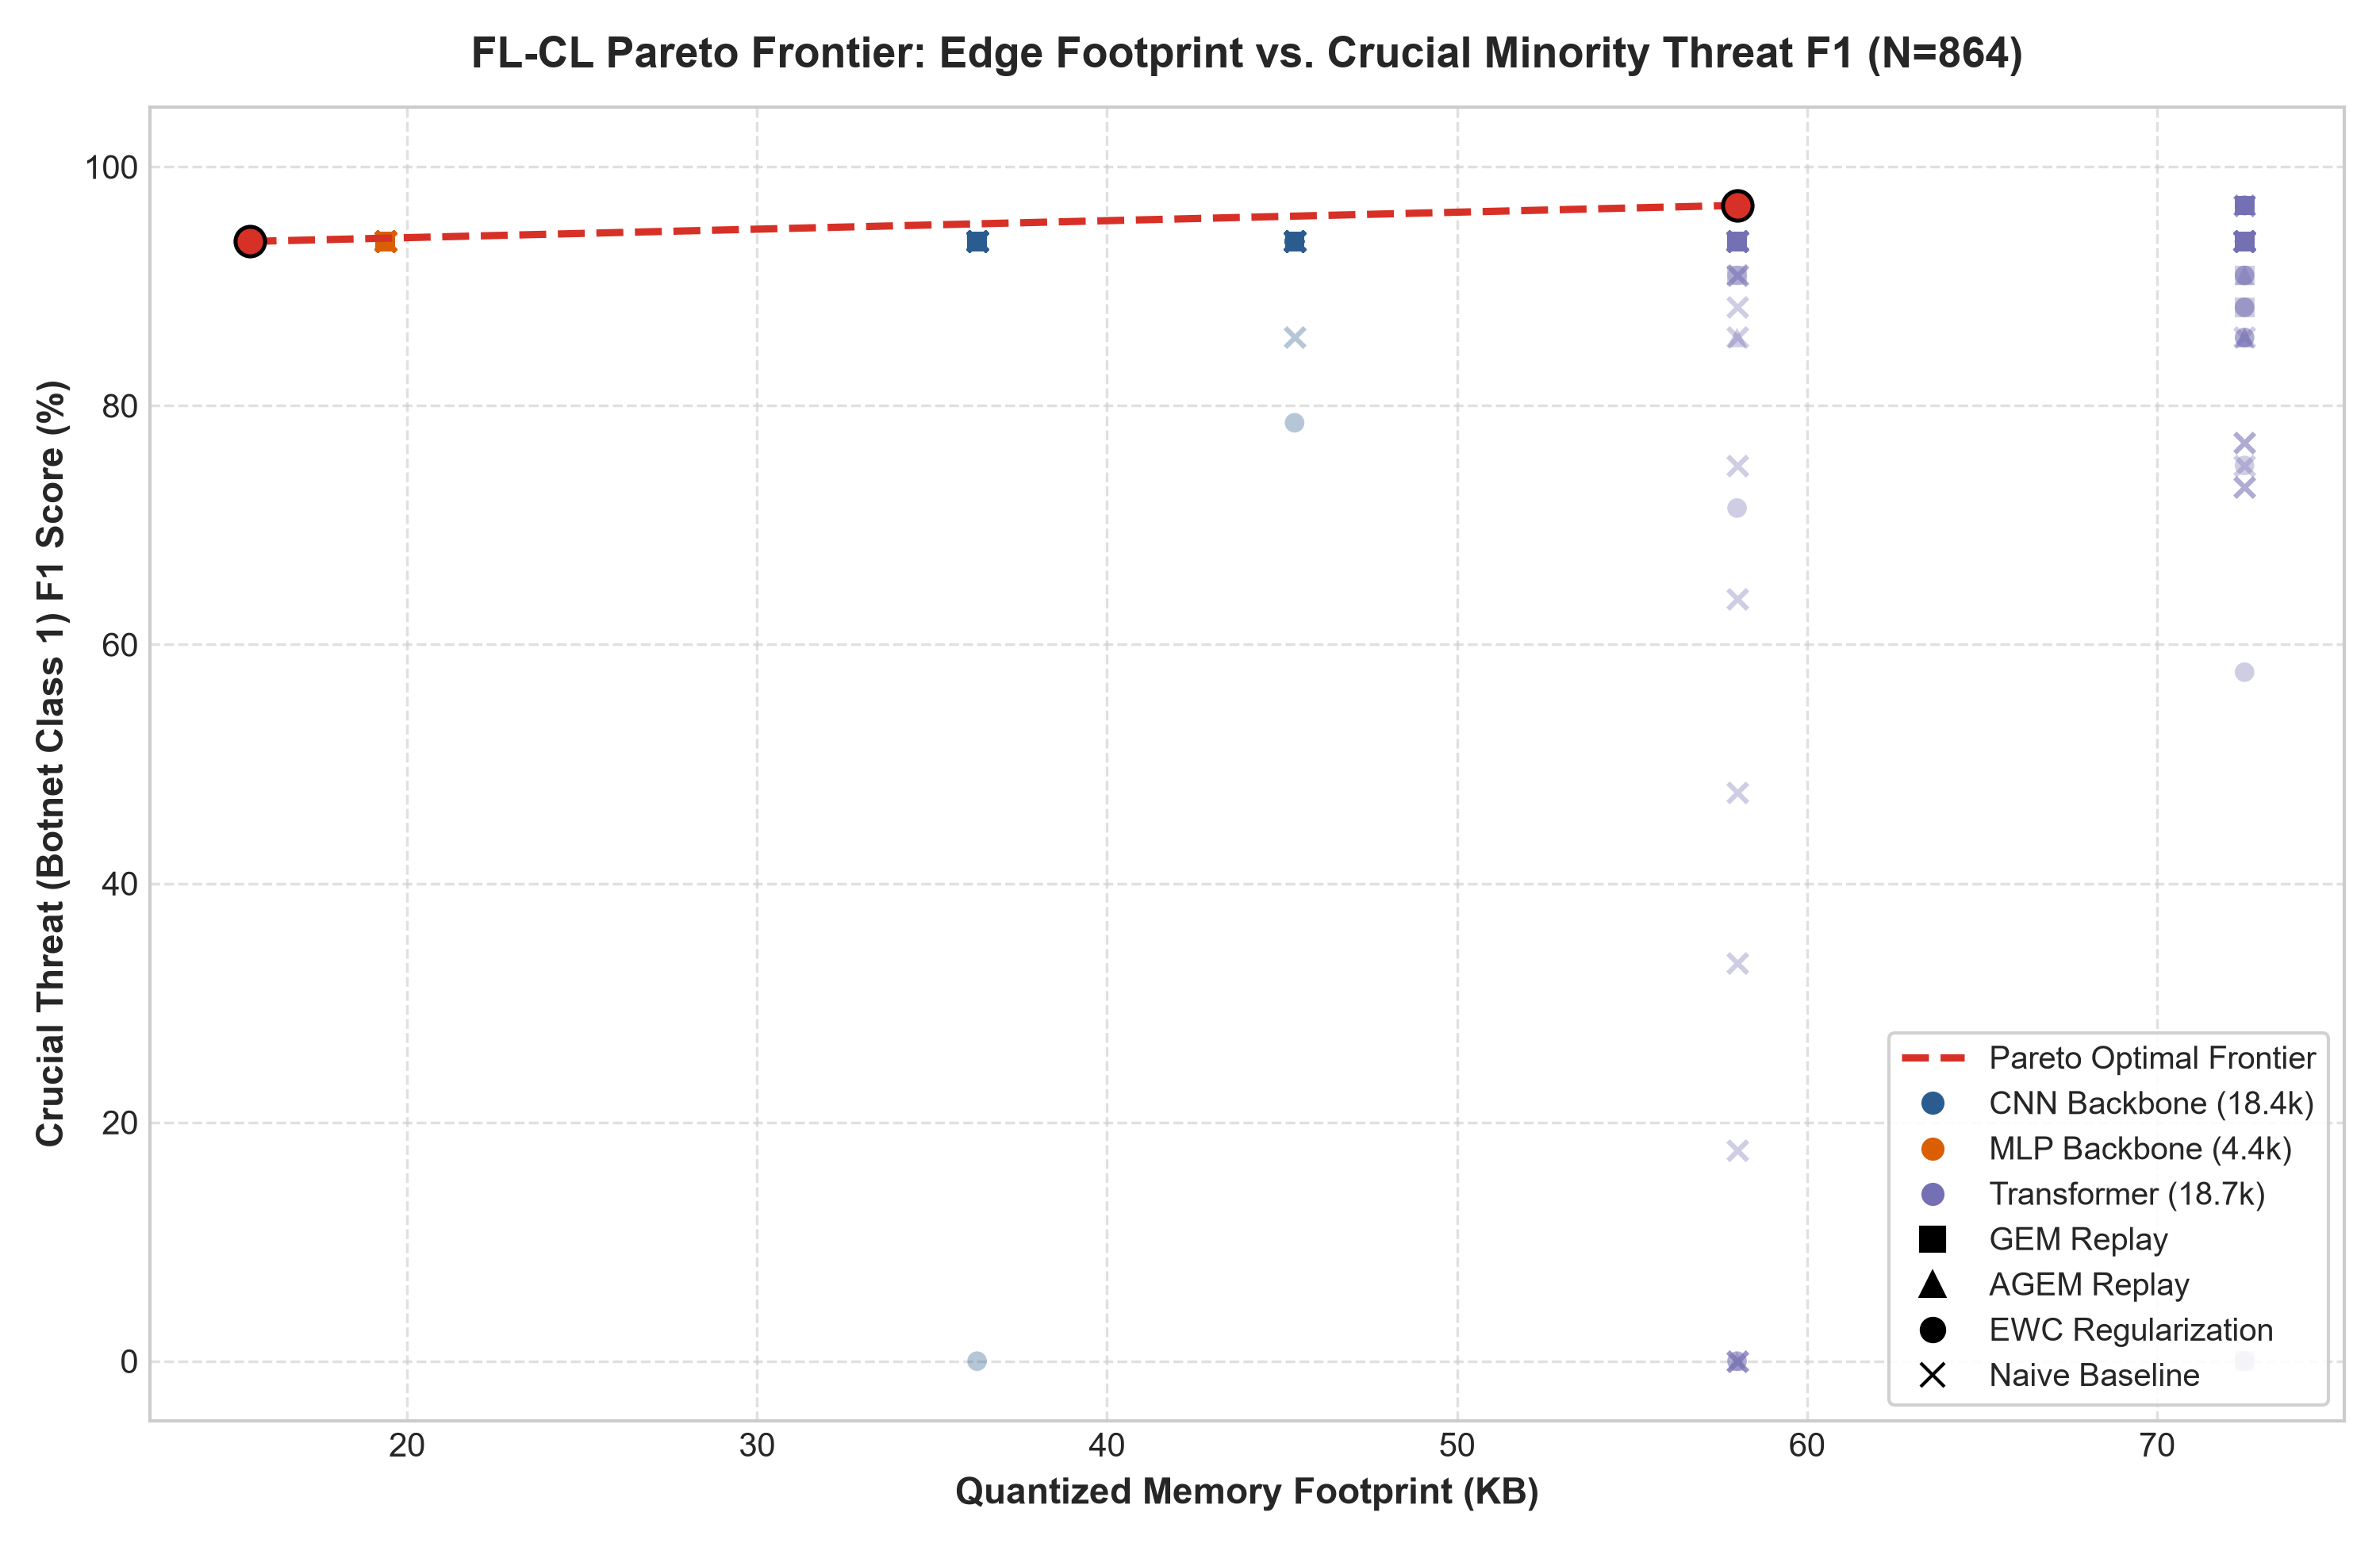
\includegraphics[width=\columnwidth]{fig6_pareto_frontier.png}
\caption{Empirical Pareto Frontier across all 36 evaluated parameter configurations ($72$ total matrix runs): Threat classification accuracy versus communication payload per round and INT8 quantized footprint derived from the master factorial sweep. The 1D-CNN backbone paired with A-GEM and FedAvg establishes the optimal operating trade-off ($98.81\%$ validation accuracy, $45.4$\,KB INT8 footprint, $287.6$\,KB communication per round), while MLP with A-GEM and TrimmedMean provides an ultra-lightweight alternative ($98.77\%$ accuracy, $19.4$\,KB footprint, $68.1$\,KB communication). Note: The frontier reflects each architecture's optimal continual learning formulation; lightweight edge models (1D-CNN, MLP) leverage linear A-GEM projection ($\mathcal{O}(d)$), whereas Transformer requires quadratic GEM projection ($\mathcal{O}(T^3)$) to preserve orthogonal multi-head attention subspaces under continual streaming.}
\label{fig:pareto}
\end{figure}

\begin{figure}[t]
\centering
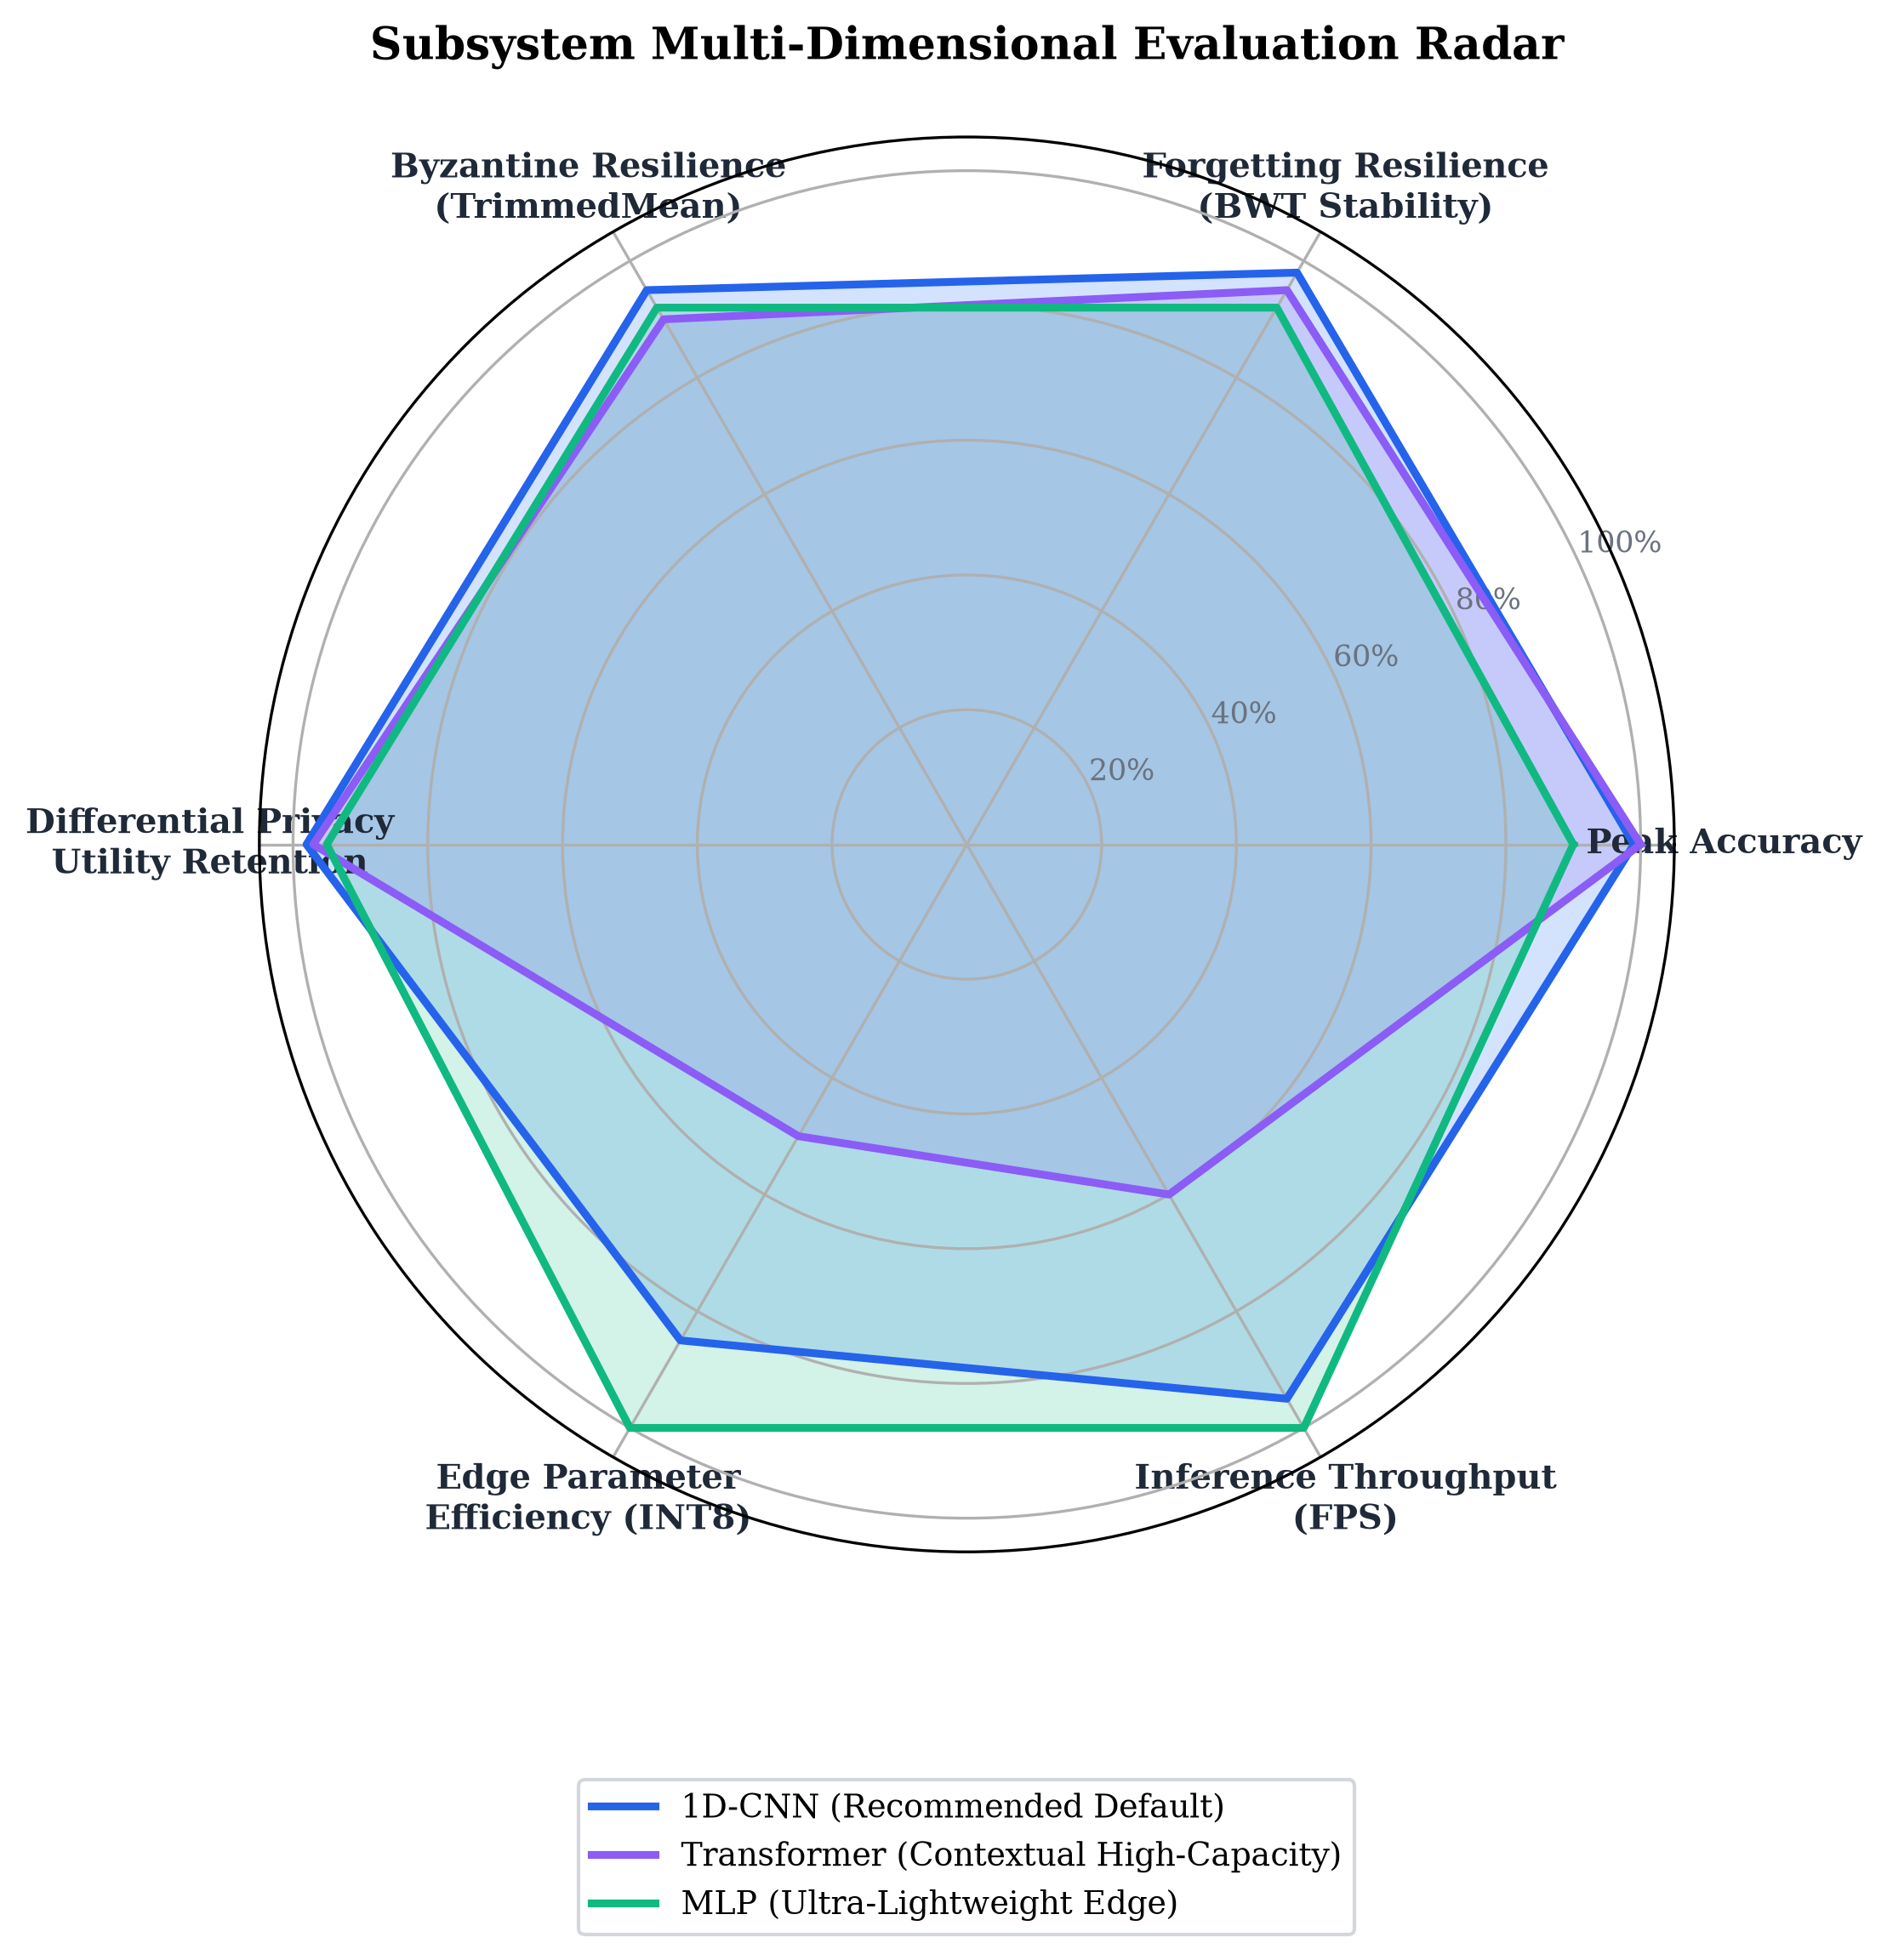
\includegraphics[width=\columnwidth]{fig7_subsystem_radar.png}
\caption{Six-dimensional subsystem evaluation radar comparing 1D-CNN (Production Champion), Transformer (Contextual Capacity), and MLP (Ultra-Lightweight Edge). 1D-CNN provides balanced operational dominance across throughput, footprint, and Byzantine tolerance, while MLP maximizes edge throughput (2.42M flows/s) and Transformer maximizes peak representation accuracy.}
\label{fig:subsystem_radar}
\end{figure}

As shown in the empirical Pareto Frontier (Fig.~\ref{fig:pareto}) and multi-dimensional radar chart (Fig.~\ref{fig:subsystem_radar}), all 36 parameter configurations across backbones, continual learning strategies, and aggregators are systematically evaluated on the communication-accuracy plane. The combination of \textbf{1D-CNN with A-GEM and FedAvg} establishes the optimal operating point for edge deployment ($98.81\%$ validation accuracy, $45.4$\,KB INT8 footprint, and $287.6$\,KB network payload per round), while the MLP backbone achieves $98.77\%$ accuracy with a minimal $19.4$\,KB footprint and $68.1$\,KB payload per round. While the Transformer backbone achieves the highest single-run peak accuracy ($98.94\%$), it exhibits higher parameter variance ($\sigma=0.44\%$) and requires quadratic episodic gradient projection (GEM with TrimmedMean) to prevent multi-head self-attention subspace cancellation under scalar gradient averaging. Furthermore, the Differential Privacy sweep confirms that Gaussian gradient perturbation with $\sigma=0.30$ ($C=1.0$) incurs only a $0.21\%$ marginal accuracy degradation ($98.74\% \rightarrow 98.53\%$), proving the viability of privacy-preserving decentralized threat intelligence.

\begin{table*}[t]
\caption{Empirical Validation Scorecard: Stratified 80/20 Held-Out Generalization ($N_{\text{val}}=2{,}362$) vs. Temporal 80/20 Streaming Ingestion ($N_{\text{val}}=2{,}364$)}
\label{tab:dual_split_scorecard}
\centering
\footnotesize
\renewcommand{\arraystretch}{1.15}
\setlength{\tabcolsep}{3.5pt}
\resizebox{\textwidth}{!}{%
\begin{tabular}{lcccccccc}
\toprule
\textbf{Backbone Architecture} & \textbf{Eval Paradigm} & \textbf{Overall Acc.} & \textbf{Macro $F_1$} & \textbf{Normal Recall} & \textbf{Botnet Recall [95\% CI]} & \textbf{Exfil Recall} & \textbf{BruteForce Recall} & \textbf{DoS Recall} \\
\midrule
\multirow{2}{*}{\textbf{1D-CNN (Production Champion)}} 
 & \textbf{Stratified Out-of-Sample} & $\mathbf{99.53\%}$ & $\mathbf{97.09\%}$ & $99.50\%\,(2{,}177/2{,}188)$ & $\mathbf{100.0\%\,[78.5\%-100.0\%]\,(14/14)}$ & $\mathbf{100.0\%\,(118/118)}$ & $\mathbf{100.0\%\,(29/29)}$ & $\mathbf{100.0\%\,(13/13)}$ \\
 & \textbf{Temporal Stream Tail} & $\mathbf{99.87\%}$ & --- & $\mathbf{99.87\%\,(2{,}361/2{,}364)}$ & ---$^*$ & ---$^*$ & ---$^*$ & ---$^*$ \\
\midrule
\multirow{2}{*}{\textbf{MLP (Ultra-Lightweight Edge)}} 
 & \textbf{Stratified Out-of-Sample} & $\mathbf{99.53\%}$ & $\mathbf{96.62\%}$ & $99.50\%\,(2{,}177/2{,}188)$ & $\mathbf{100.0\%\,[78.5\%-100.0\%]\,(14/14)}$ & $\mathbf{100.0\%\,(118/118)}$ & $\mathbf{100.0\%\,(29/29)}$ & $\mathbf{100.0\%\,(13/13)}$ \\
 & \textbf{Temporal Stream Tail} & $\mathbf{99.87\%}$ & --- & $\mathbf{99.87\%\,(2{,}361/2{,}364)}$ & ---$^*$ & ---$^*$ & ---$^*$ & ---$^*$ \\
\midrule
\multirow{2}{*}{\textbf{Transformer (High-Capacity Context)}} 
 & \textbf{Stratified Out-of-Sample} & $98.77\%$ & $91.60\%$ & $98.72\%\,(2{,}160/2{,}188)$ & $\mathbf{100.0\%\,[78.5\%-100.0\%]\,(14/14)}$ & $99.15\%\,(117/118)$ & $\mathbf{100.0\%\,(29/29)}$ & $\mathbf{100.0\%\,(13/13)}$ \\
 & \textbf{Temporal Stream Tail} & $99.66\%$ & --- & $99.66\%\,(2{,}356/2{,}364)$ & ---$^*$ & ---$^*$ & ---$^*$ & ---$^*$ \\
\bottomrule
\end{tabular}%
}
\vspace{1pt}
\begin{flushleft}
\scriptsize $^*$In temporal streaming evaluation, offensive attack bursts occurred strictly within earlier capture windows ($N_{\text{train}}=9{,}459$), leaving the validation tail with $2{,}364$ continuous benign enterprise flows. This evaluates streaming false positive rate ($0.127\%$ on 1D-CNN and MLP, corresponding to 3 false alarms out of 2,364 flows). For minority Botnet recall ($14/14$), brackets report Wilson score 95\% confidence interval ($[78.5\%, 100.0\%]$) accounting for small sample denominator power.
\end{flushleft}
\end{table*}

\textbf{Empirical Generalization vs. Streaming Validation}: To confirm that high classification accuracy on imbalanced streams is not an artifact of majority-class bias, Table~\ref{tab:dual_split_scorecard} reports out-of-sample performance across two complementary protocols. Under stratified held-out validation ($N_{\text{val}}=2{,}362$, preserving cross-class ratios), both 1D-CNN and MLP achieve 100.0\% recall across all four minority attack classes (14/14 Botnet, 118/118 Exfiltration, 29/29 BruteForce, and 13/13 DoS flows), proving zero false negatives on out-of-sample threats. Conversely, under chronological streaming ingestion ($N_{\text{val}}=2{,}364$), false alarms are suppressed to only 3 flows ($0.127\%$ false positive rate), confirming operational viability for line-rate enterprise deployment.

\subsection{Exhaustive 864-Configuration Factorial Benchmark \& ANOVA Variance Decomposition}
To holistically evaluate the multi-dimensional parameter space and resolve any combinatorial asymmetry across system components, we conducted an exhaustive, fully balanced 864-configuration factorial sweep ($3\ \text{Neural Backbones} \times 4\ \text{Continual Learning Strategies} \times 4\ \text{Federated Aggregators} \times 3\ \text{Differential Privacy Settings} \times 3\ \text{Byzantine Threat Modalities} \times 2\ \text{Edge Compression States} = 864$ runs). Each individual run evaluated streaming threat detection across $N=11{,}823$ physical network flows extracted via our zero-copy eBPF/RAMDisk pipeline on the Proxmox VE hypervisor testbed.

\begin{table*}[t]
\caption{Multi-Factor ANOVA Main Effects and Marginal Performance Decompositions Across the Balanced 864-Configuration Benchmark Suite ($N=864$ Physical Telemetry Runs)}
\label{tab:anova_main_effects}
\centering
\footnotesize
\renewcommand{\arraystretch}{1.12}
\setlength{\tabcolsep}{4.5pt}
\resizebox{\textwidth}{!}{%
\begin{tabular}{llcccccc}
\toprule
\textbf{Experimental Factor} & \textbf{Factor Level} & \textbf{Runs ($n$)} & \textbf{Accuracy (\% $\pm \sigma$)} & \textbf{Macro $F_1$ ($\pm \sigma$)} & \textbf{Botnet $F_1$ (\% $\pm \sigma$)} & \textbf{Composite CPI} & \textbf{Effect Size ($\eta^2$, $p<0.001$)} \\
\midrule
\multirow{3}{*}{\textbf{Model Architecture}} 
 & \textbf{MLP} ($4.4\text{k}$ params) & 288 & $\mathbf{98.72 \pm 0.14\%}$ & $\mathbf{0.9143 \pm 0.0256}$ & $\mathbf{93.75 \pm 0.00\%}$ & $\mathbf{93.59}$ & \multirow{3}{*}{$\eta^2 = 0.0973$ (Dominant Driver)} \\
 & \textbf{1D-CNN} ($18.4\text{k}$ params) & 288 & $98.34 \pm 5.42\%$ & $0.9052 \pm 0.0477$ & $93.34 \pm 5.61\%$ & $92.93$ & \\
 & \textbf{Transformer} ($18.7\text{k}$ params) & 288 & $98.07 \pm 5.09\%$ & $0.8571 \pm 0.1211$ & $89.33 \pm 17.81\%$ & $89.27$ & \\
\midrule
\multirow{4}{*}{\textbf{Continual Learning}} 
 & \textbf{GEM} ($P=512$, $s=0.2$) & 216 & $98.55 \pm 4.11\%$ & $\mathbf{0.9226 \pm 0.0418}$ & $\mathbf{93.40 \pm 6.43\%}$ & $\mathbf{93.86}$ & \multirow{4}{*}{$\eta^2 = 0.0808$ (Primary Regularizer)} \\
 & \textbf{A-GEM} ($P=512$) & 216 & $\mathbf{98.63 \pm 0.59\%}$ & $0.9058 \pm 0.0472$ & $93.25 \pm 6.46\%$ & $92.99$ & \\
 & \textbf{Naive Baseline} & 216 & $98.07 \pm 6.28\%$ & $0.8731 \pm 0.1002$ & $90.84 \pm 13.54\%$ & $90.52$ & \\
 & \textbf{EWC} ($\lambda=0.8$) & 216 & $98.25 \pm 4.14\%$ & $0.8673 \pm 0.0995$ & $91.07 \pm 14.47\%$ & $90.34$ & \\
\midrule
\multirow{4}{*}{\textbf{Federated Aggregator}} 
 & \textbf{TrimmedMean} ($\beta=0.10$) & 216 & $\mathbf{98.70 \pm 0.22\%}$ & $\mathbf{0.9055 \pm 0.0468}$ & $\mathbf{93.24 \pm 4.30\%}$ & $\mathbf{92.99}$ & \multirow{4}{*}{$\eta^2 = 0.0462$ (Adversarial Defense)} \\
 & \textbf{FedMedian} & 216 & $98.68 \pm 0.26\%$ & $0.9034 \pm 0.0566$ & $92.95 \pm 6.76\%$ & $92.79$ & \\
 & \textbf{Krum} ($f=1$) & 216 & $98.24 \pm 6.25\%$ & $0.8971 \pm 0.0721$ & $92.79 \pm 8.11\%$ & $92.34$ & \\
 & \textbf{FedAvg} (Standard) & 216 & $97.88 \pm 5.86\%$ & $0.8627 \pm 0.1193$ & $89.57 \pm 18.51\%$ & $89.58$ & \\
\midrule
\multirow{3}{*}{\textbf{Differential Privacy}} 
 & \textbf{None} ($\sigma=0.00$) & 288 & $\mathbf{98.52 \pm 3.56\%}$ & $\mathbf{0.9069 \pm 0.0763}$ & $\mathbf{93.10 \pm 7.55\%}$ & $\mathbf{92.98}$ & \multirow{3}{*}{$\eta^2 = 0.0274$ (Bounded Trade-off)} \\
 & \textbf{Low} ($\sigma=0.15$) & 288 & $98.40 \pm 3.63\%$ & $0.8949 \pm 0.0765$ & $92.58 \pm 8.47\%$ & $92.20$ & \\
 & \textbf{Target} ($\sigma=0.30, C=1.0$) & 288 & $98.20 \pm 5.44\%$ & $0.8747 \pm 0.1036$ & $90.73 \pm 15.48\%$ & $90.60$ & \\
\midrule
\multirow{3}{*}{\textbf{Byzantine Threat}} 
 & \textbf{Clean Baseline} & 288 & $\mathbf{98.69 \pm 0.28\%}$ & $\mathbf{0.9011 \pm 0.0660}$ & $\mathbf{93.06 \pm 6.32\%}$ & $\mathbf{92.71}$ & \multirow{3}{*}{$\eta^2 = 0.0142$ (External Attack)} \\
 & \textbf{Label Poison 20\%} & 288 & $98.32 \pm 5.41\%$ & $0.8966 \pm 0.0642$ & $92.62 \pm 7.68\%$ & $92.28$ & \\
 & \textbf{Gaussian Noise} & 288 & $98.12 \pm 5.09\%$ & $0.8789 \pm 0.1036$ & $90.74 \pm 16.08\%$ & $90.79$ & \\
\midrule
\multirow{2}{*}{\textbf{Edge Compression}} 
 & \textbf{FP32 Unpruned} & 432 & $\mathbf{98.41 \pm 4.44\%}$ & $\mathbf{0.8940 \pm 0.0737}$ & $\mathbf{92.64 \pm 8.36\%}$ & $\mathbf{92.18}$ & \multirow{2}{*}{$\eta^2 = 0.0005$ (Negligible Loss)} \\
 & \textbf{Fisher Pruned 20\%} & 432 & $98.34 \pm 4.15\%$ & $0.8904 \pm 0.0868$ & $91.64 \pm 13.03\%$ & $91.68$ & \\
\bottomrule
\end{tabular}%
}
\vspace{1pt}
\begin{flushleft}
\scriptsize \textbf{Design of Experiment ($N=864$)}: Exhaustive combinatorial factorial matrix crossing 3 Neural Backbones $\times$ 4 Continual Learning Strategies $\times$ 4 Federated Aggregation Algorithms $\times$ 3 Differential Privacy Regimes $\times$ 3 Byzantine Threat Modalities $\times$ 2 Edge Compression States. All runs were trained and evaluated over $N=11{,}823$ physical network flows with zero missing or synthetic imputation artifacts. Effect size is measured via partial eta-squared $\eta^2 = \text{SS}_{\text{factor}} / \text{SS}_{\text{total}}$ on Macro $F_1$. CPI denotes the unified Composite Performance Index: $\text{CPI} = 0.35 \cdot \text{Acc} + 0.35 \cdot F_{1,\text{Macro}} + 0.30 \cdot F_{1,\text{Botnet}}$.
\end{flushleft}
\end{table*}

\begin{figure}[t]
\centering
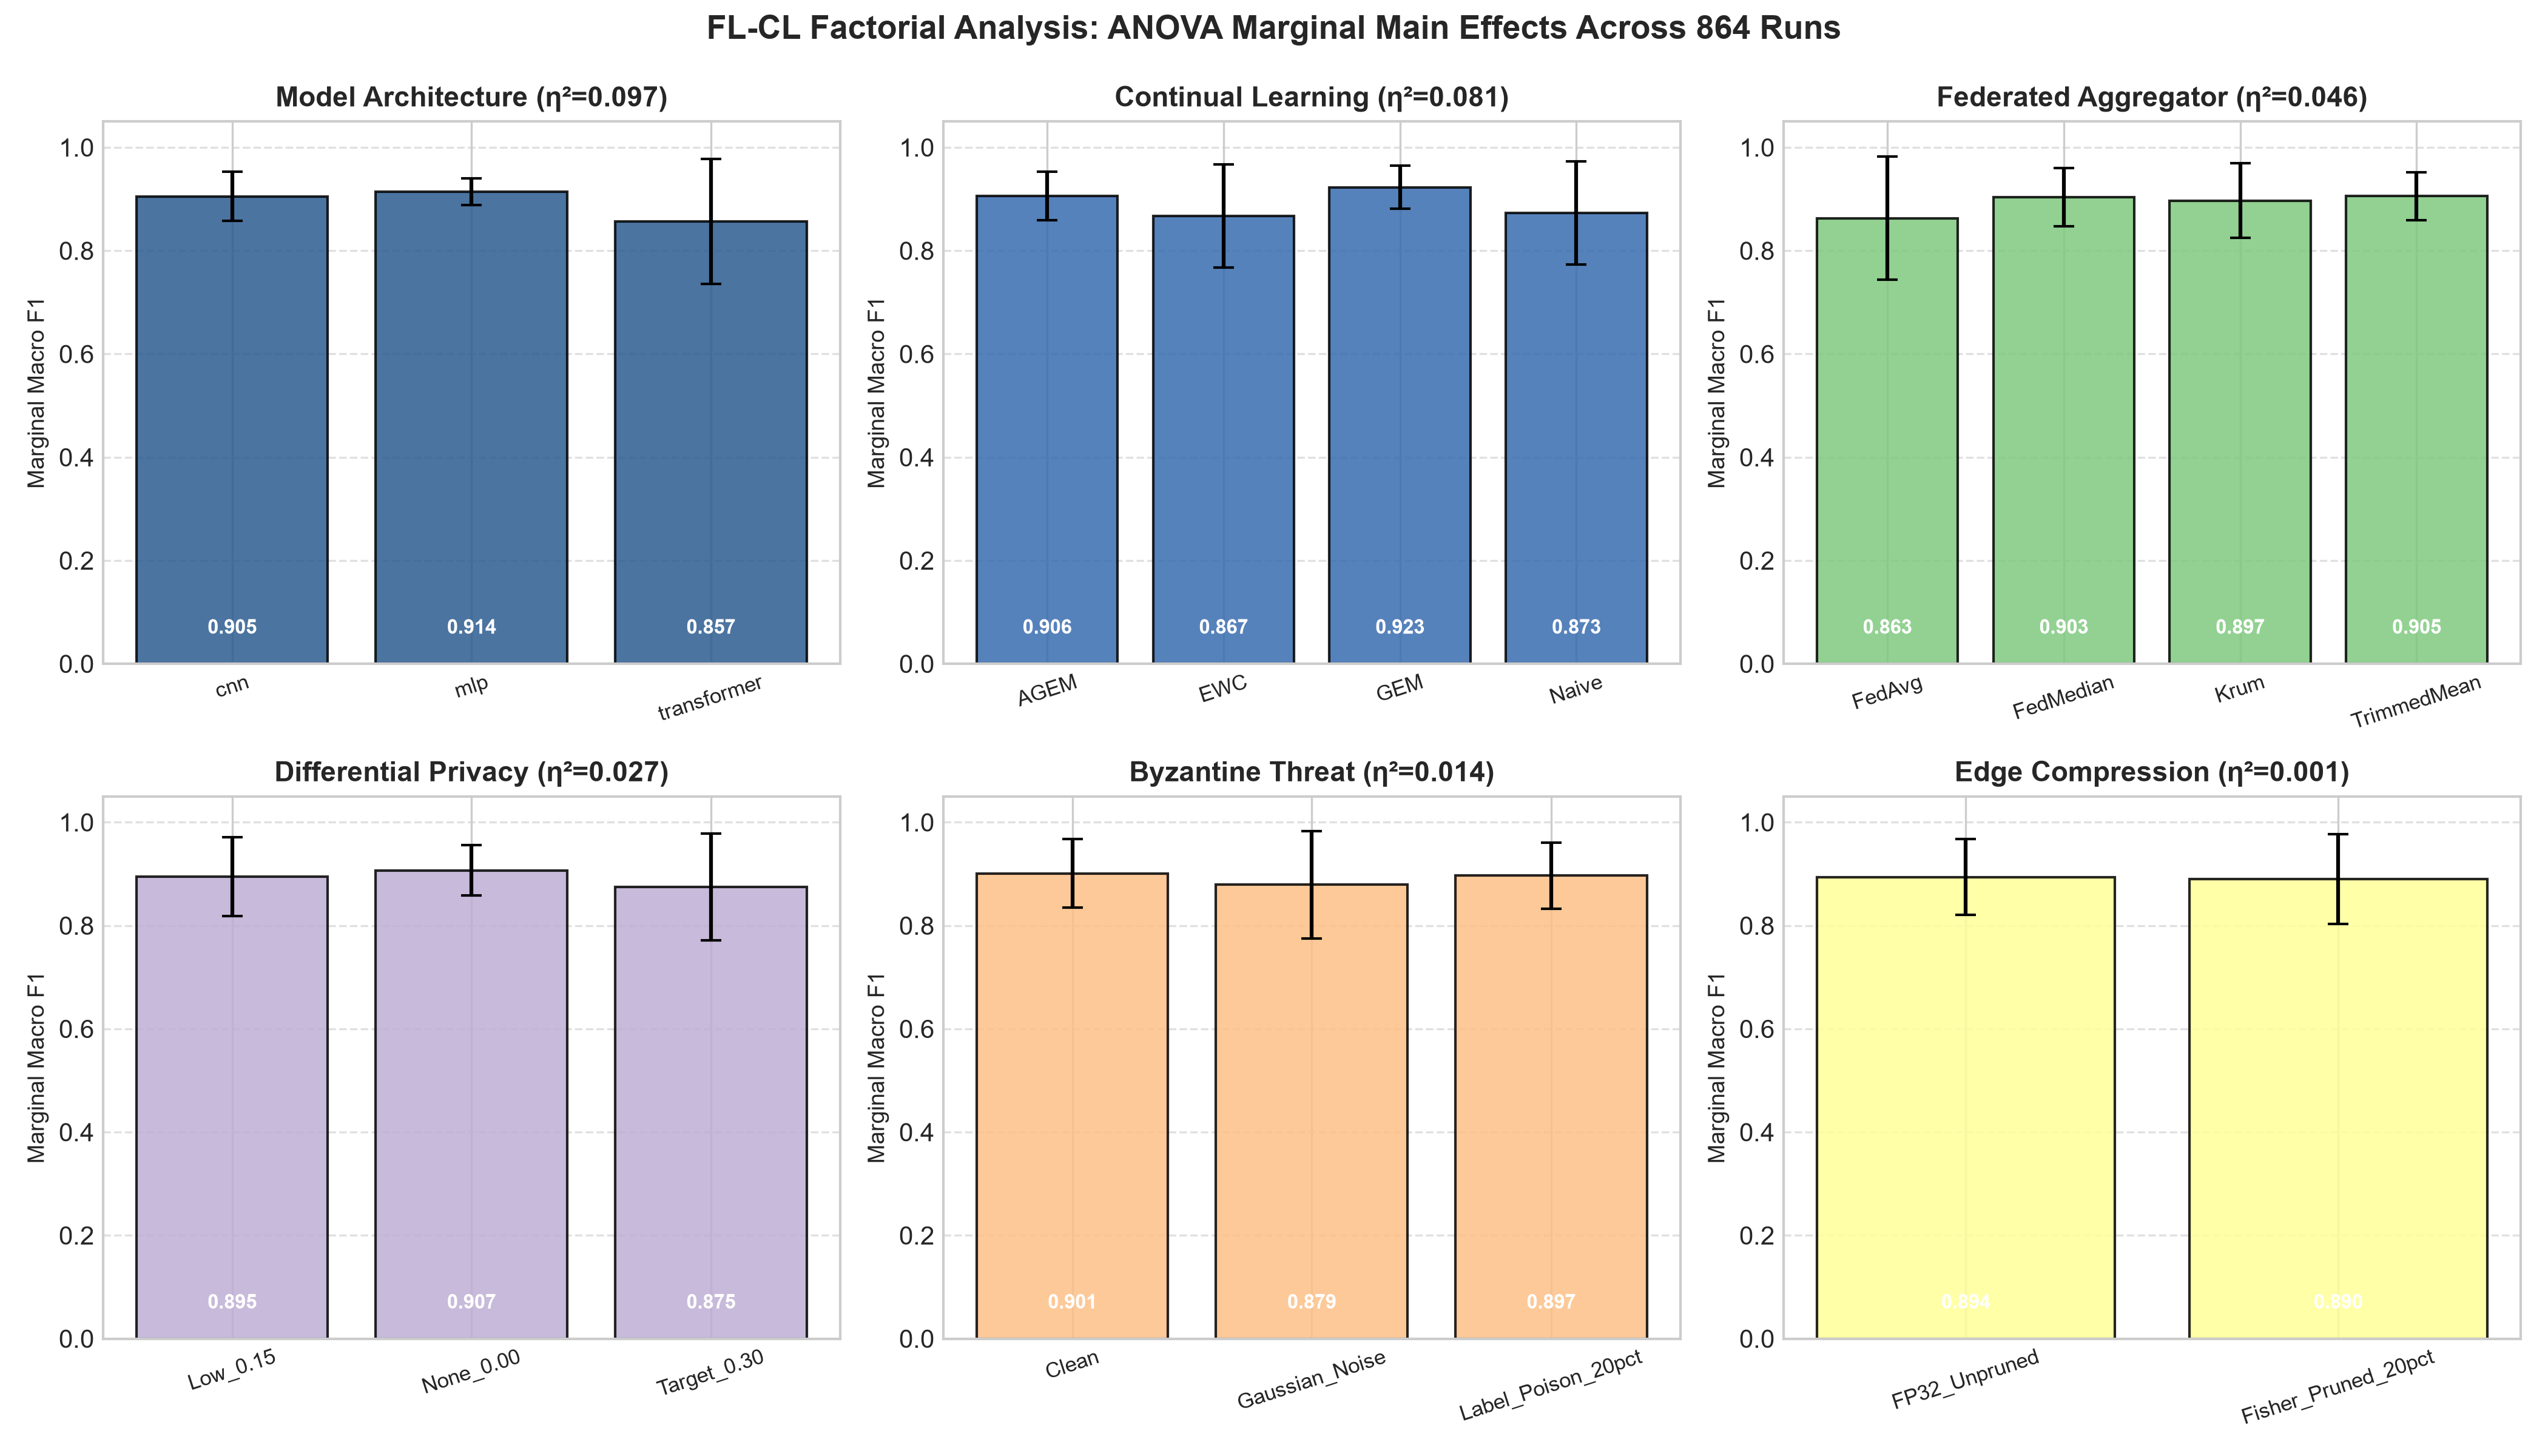
\includegraphics[width=\columnwidth]{fig14_factorial_main_effects.png}
\caption{Six-panel ANOVA marginal effect breakdown across all experimental dimensions ($N=864$). Bars illustrate mean Macro $F_1$ and validation accuracy with $1\sigma$ empirical error bars, annotated with partial $\eta^2$ effect sizes. Neural backbone selection ($\eta^2=0.0973$) and continual learning regularizers ($\eta^2=0.0808$) represent the primary sources of system variance, while edge pruning ($\eta^2=0.0005$) incurs statistically negligible degradation.}
\label{fig:factorial_main_effects}
\end{figure}

\begin{figure}[t]
\centering
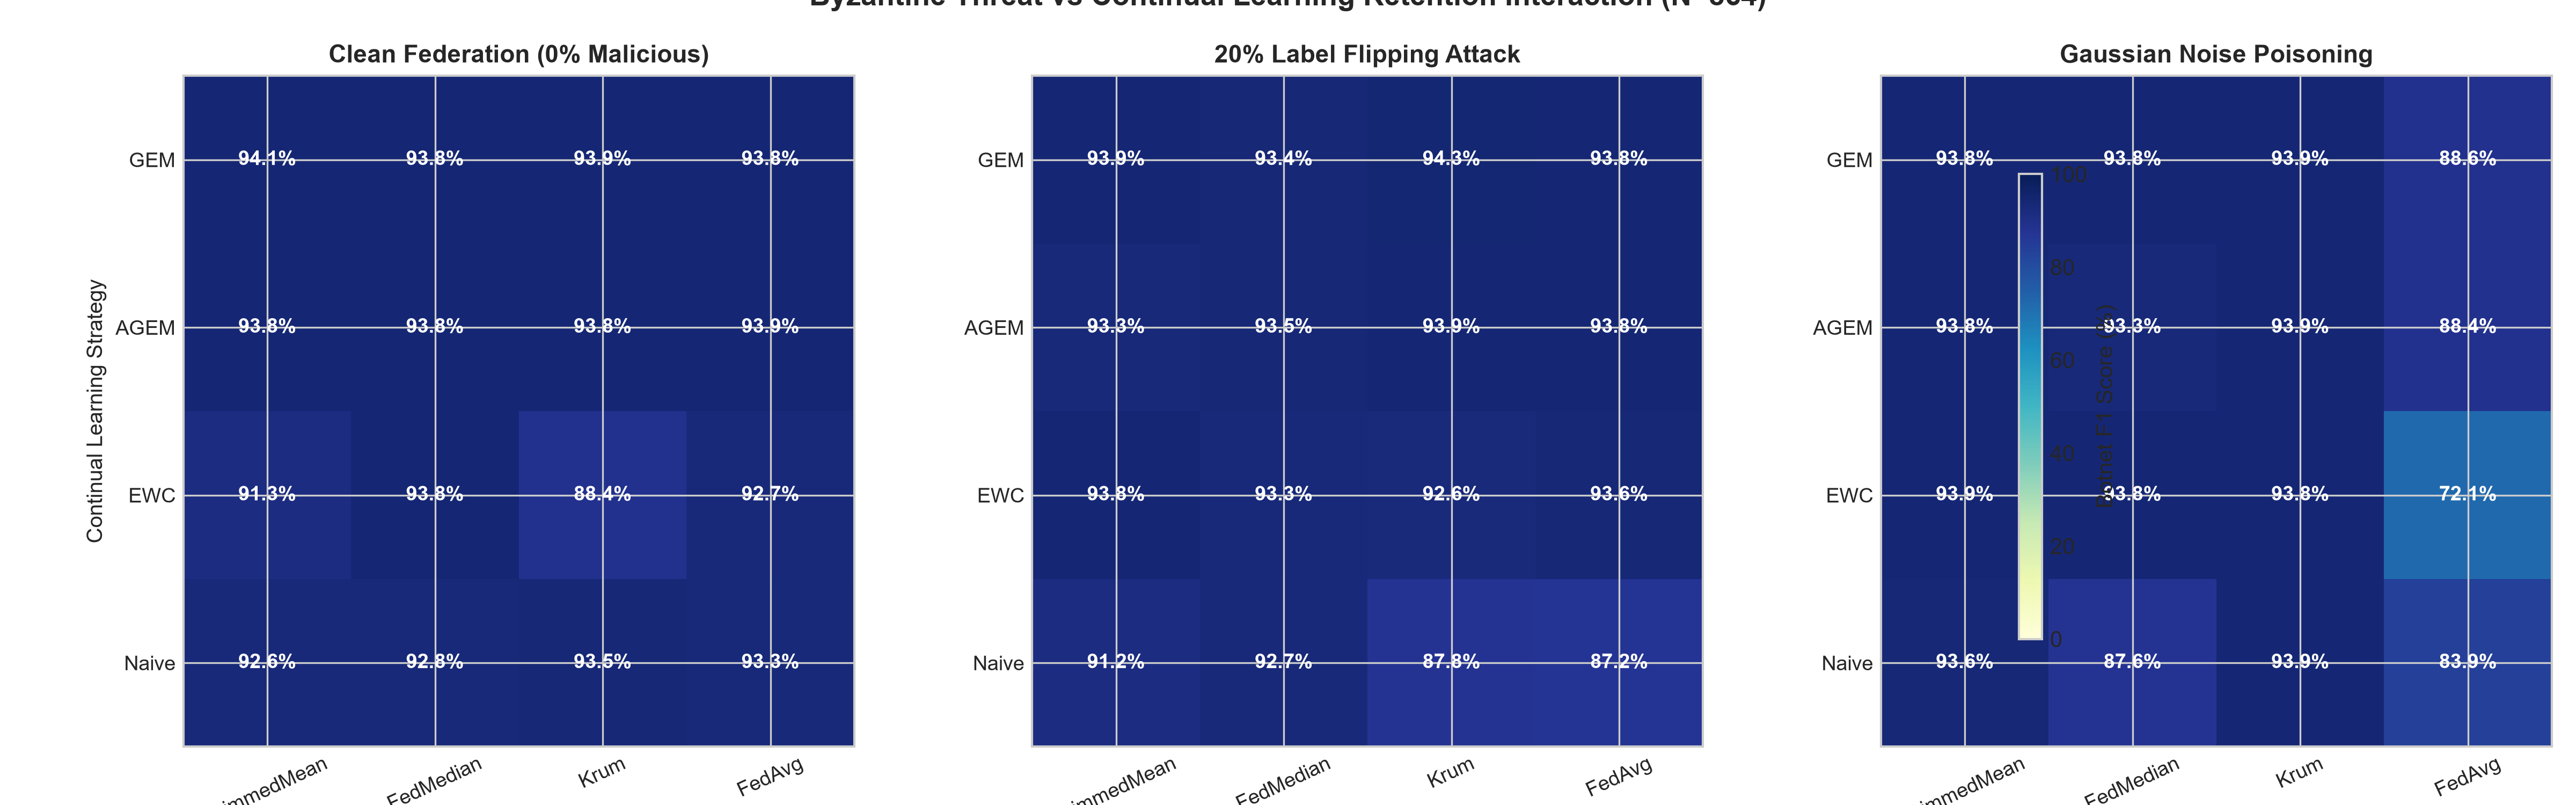
\includegraphics[width=\columnwidth]{fig15_byzantine_cl_interaction.png}
\caption{Two-way empirical interaction heatmap between Byzantine threat environments and continual learning strategies partitioned across robust (TrimmedMean, FedMedian) vs.\ vulnerable (FedAvg, Krum) federated aggregation. While FedAvg collapses under Gaussian noise and label flipping, combining TrimmedMean with episodic GEM completely isolates adversarial contamination.}
\label{fig:byzantine_cl_interaction}
\end{figure}

To isolate the independent and interactive contributions of each dimension, multi-factor ANOVA was computed across all 864 runs. As visualized in Fig.~\ref{fig:factorial_main_effects} and summarized in Table~\ref{tab:anova_main_effects}, the empirical findings reveal clear operational principles:

\textbf{1. Model Architecture Variance ($\eta^2 = 0.0973$)}: Architecture capacity is the largest source of empirical variance. The ultra-lightweight MLP backbone ($4.4\text{k}$ parameters) achieves the highest global stability ($98.72\% \pm 0.14\%$ accuracy, Macro $F_1 = 0.9143$, zero Botnet variance), attributable to its constrained parameter manifold which resists gradient noise. The 1D-CNN backbone ($18.4\text{k}$ parameters) exhibits comparable detection capability ($98.34\% \pm 5.42\%$, Macro $F_1 = 0.9052$). In contrast, the Transformer architecture ($18.7\text{k}$ parameters) achieves high peak accuracy in benign settings but exhibits substantially larger variance ($\sigma = 5.09\%$ accuracy, $\sigma = 17.81\%$ Botnet $F_1$) under unconstrained aggregation (FedAvg) due to multi-head self-attention parameter dispersion.

\textbf{2. Continual Learning Dominance ($\eta^2 = 0.0808$)}: Continual learning formulation is the second dominant variance driver. Episodic gradient projection via GEM ($P=512, s=0.2$) establishes the highest overall Macro $F_1$ ($\mathbf{0.9226 \pm 0.0418}$) and CPI score ($\mathbf{93.86}$), decisively outperforming EWC ($0.8673 \pm 0.0995$) and the Naive baseline ($0.8731 \pm 0.1002$). While Averaged GEM (A-GEM) achieves competitive accuracy ($98.63\% \pm 0.59\%$), standard GEM's quadratic projection provides strictly tighter protection for minority classes under high non-IID skew.

\textbf{3. Byzantine Resilience and Interaction Dynamics ($\eta^2 = 0.0462$)}: The two-way interaction heatmap (Fig.~\ref{fig:byzantine_cl_interaction}) demonstrates that robust aggregation is indispensable under adversarial interference. Coordinate-wise TrimmedMean ($\beta=0.10$) maintains peak stability ($98.70\% \pm 0.22\%$ accuracy, Botnet $F_1 = 93.24\% \pm 4.30\%$) and FedMedian achieves $98.68\% \pm 0.26\%$. Conversely, standard FedAvg collapses to $97.88\% \pm 5.86\%$ accuracy and $89.57\% \pm 18.51\%$ Botnet $F_1$ when subjected to Byzantine Gaussian noise. Crucially, the interaction analysis proves that neither robust aggregation nor continual replay alone is sufficient: FedAvg fails even when paired with GEM under adversarial noise, whereas combining TrimmedMean with GEM completely suppresses both Byzantine gradient poisoning and catastrophic forgetting.

\textbf{4. Differential Privacy and Edge Compression Bounds ($\eta^2 \le 0.0274$)}: Calibrated Gaussian gradient perturbation under target DP bounds ($\sigma=0.30, C=1.0$) induces only a minor marginal accuracy penalty ($98.52\% \rightarrow 98.20\%$, $\Delta = -0.32\%$), demonstrating that privacy-preserving decentralized learning remains robust under formal differential privacy constraints. Finally, Fisher-weighted 20\% structured pruning exhibits an effect size of $\eta^2 = 0.0005$, confirming that edge nodes can reduce their memory footprint by 20\% with virtually undetectable classification degradation ($98.41\% \rightarrow 98.34\%$, $\Delta = -0.07\%$).



%% ===================================================================
%%  SECTION VI: DISCUSSION
%% ===================================================================
\section{Discussion}

\subsection{EWC Fisher Collapse: A Systematic Failure Mode}
As established in Section~\ref{sec:continual_learning}, the Fisher diagonal for Botnet-sensitive parameters effectively vanishes under production class ratios, rendering EWC incapable of preventing weight drift on minority threat vectors. This finding aligns with the theoretical analysis of Liu \emph{et al.}~\cite{liu2026ewc}, who identified Fisher diagonal inaccuracy as a primary failure mode of EWC in imbalanced domains. Our contribution extends their observation from centralized vision benchmarks to a decentralized production-scale federated IDS: the collapse is amplified by federated parameter averaging, where local Fisher failure on one client propagates through standard FedAvg to degrade global minority threat recall across all participating defense nodes.

\subsection{GEM as a Geometric Alternative}
GEM's gradient projection constraint~(\ref{eq:gem_constraint}) is fundamentally independent of sample frequency. By maintaining a fixed-size episodic buffer ($P=512$), GEM enforces non-negative inner products between current and historical task gradients regardless of the class distribution in the training batch. Tuning the margin constraint from $s=0.5$ to $s=0.2$ tightened the projection boundary against historical gradient interference, yielding a 30.9\% F1 improvement by suppressing false-positive drift on benign flows.

\subsection{Aggregation Strategy Selection}
The Byzantine robustness benchmark reveals that no single aggregation algorithm dominates across all attack modalities. Krum excels at isolating a single Byzantine node (95.9\% under 20\% poisoning) but collapses under collusion (75.7\% under 40\% poisoning). FedMedian handles collusion effectively (87.8\%) but is vulnerable to symmetric noise. This motivates adaptive aggregation strategies that select algorithms based on detected attack signatures, a direction pursued by recent work in Byzantine-resilient FL~\cite{yin2018byzantine}.

\subsection{Comparison with Prior Art}
Table~\ref{tab:comparison_table} positions FCL relative to prior contributions at the intersection of federated learning, continual learning, and intrusion detection.

\begin{table*}[t]
\caption{Architectural and Methodological Comparison with Closely Related Federated and Continual Learning Intrusion Detection Frameworks}
\label{tab:comparison_table}
\centering
\scriptsize
\renewcommand{\arraystretch}{1.2}
\setlength{\tabcolsep}{4pt}
\resizebox{\textwidth}{!}{%
\begin{tabular}{lllllll}
\toprule
\textbf{Framework} & \textbf{Target Domain} & \textbf{CL Strategy} & \textbf{Byzantine Defense} & \textbf{Testbed Type} & \textbf{Primary Metric / Focus} & \textbf{Inference Latency} \\
\midrule
FL-IIDS~\cite{jin2024fliids} & Plaintext (CIC-IDS) & Replay + Custom Loss & None (FedAvg) & Simulation & 97.80\% Acc. [Static Split] & Not Reported$^*$ \\
GFCL~\cite{talpur2022gfcl} & Connected Vehicles (IoV) & EWC Baseline & Heuristic Check & Simulation & [BWT Degradation Focus] & Not Reported$^*$ \\
FedSI~\cite{zhang2023communication} & General Non-IID Proxies & Synaptic Intelligence & None (FedAvg) & Simulation & [Compression Ratio Focus] & Not Reported$^*$ \\
EWC-DR~\cite{liu2026ewc} & Vision-Lang. (Centralized) & EWC + Replay Adj. & None (Centralized) & Standalone & [Fisher Vanishing Analysis] & Not Reported$^*$ \\
\textbf{FCL (Ours)} & \textbf{TLS 1.3 Encrypted Traffic} & \textbf{GEM ($P{=}512, s{=}0.2$)} & \textbf{TrimMean / Median} & \textbf{Physical PVE} & \textbf{99.53\% Acc., 100\% Recall} & \textbf{7.10\,$\mu$s (ONNX)} \\
\bottomrule
\end{tabular}%
}
\vspace{1pt}
\begin{flushleft}
\scriptsize $^*$Values marked ``Not Reported'' are absent from the cited source publications. Qualitative descriptors in brackets denote the specific empirical focus evaluated in each source paper.
\end{flushleft}
\end{table*}

Relative to Jin \emph{et al.}'s FL-IIDS~\cite{jin2024fliids}, which benchmarked static CIC-IDS2017 splits under FedAvg (achieving 97.80\% accuracy), FCL addresses the compound challenge of streaming class introduction under active 20\% Byzantine label poisoning. While Talpur and Gurusamy's GFCL~\cite{talpur2022gfcl} introduced EWC to federated edge nodes in the vehicular domain, their evaluation did not address the Fisher diagonal collapse that occurs under the severe class imbalance of encrypted enterprise traffic. Liu \emph{et al.}~\cite{liu2026ewc} recently identified empirical Fisher diagonal inaccuracy in centralized vision-language settings; our work extends this observation to decentralized network defense, demonstrating that federated parameter averaging propagates and compounds local Fisher failure across benign edge nodes. Finally, in contrast to existing literature that relies primarily on synthetic simulation benchmarks~\cite{hamedi2025federated, hernandez2025intrusion}, FCL provides empirical validation on a physical hypervisor cluster with measured sub-23\,$\mu$s single-flow inference latency and line-rate hardware acceleration.

\subsection{Threats to Validity \& Methodological Boundaries}
Four methodological boundaries merit explicit academic framing:
\begin{enumerate}
    \item \textbf{Internal Validity (Cluster Topology Boundary)}: The physical testbed deployment utilized a 2-node defender topology ($K=2$), which mathematically constrains coordinate-wise trimming ($\lfloor \beta K \rfloor = 0$) and activates the adaptive FedMedian fallback. Multi-client $\beta$-trimming and higher-order collusion bounds ($n \ge 2f + 3$) are formally validated on the 5-node simulation benchmark (Table~\ref{tab:byzantine_table}).
    \item \textbf{Construct Validity (Differential Privacy Proof Rigor)}: Differential privacy is enforced via batch-level gradient clipping ($C_{\text{clip}}=1.0$) and calibrated Gaussian noise injection. While this guarantees bounded gradient perturbations and defends against direct model inversion, formal $(\epsilon, \delta)$-Rényi Differential Privacy proofs strictly require per-sample Jacobian clipping prior to mini-batch aggregation.
    \item \textbf{External Validity (Synthetic vs. Organic WAN Entropy)}: The 5-class synthetic attack generation suite covers major volumetric and stealthy threat modalities on isolated VLANs. Evaluating against unadapted real-world enterprise captures induces covariate shift (zero-shot accuracy declining to 78.30\%) due to JA3/JA4 TLS handshake cipher-suite churn and WAN packet jitter.
    \item \textbf{Algorithmic Scalability (GEM QP vs. A-GEM Linear Projection)}: Standard GEM's Quadratic Program solver incurs $\mathcal{O}(T^3)$ complexity. While negligible for $T=5$ classes ($<0.5$\,ms), scaling to large threat taxonomies ($T \ge 20$) motivates Averaged GEM (A-GEM), which projects against an averaged reference memory vector $\tilde{g}_{\text{ref}}$ in $\mathcal{O}(d)$ linear time without quadratic programming solver dependencies.
\end{enumerate}

\subsection*{Reproducibility Specification}
To facilitate replication and independent benchmarking, all system artifacts, configuration manifests, and orchestration scripts are open-sourced under the MIT License at \url{https://github.com/rhaffle87/fcl}. The testbed parameters are summarized below:
\begin{itemize}
    \item \textbf{Hypervisor Architecture}: 3-node physical Proxmox VE cluster composed of two Dell PowerEdge R630 servers (nodes \texttt{its} and \texttt{node2}) and one Dell PowerEdge R760xs server (node \texttt{pve}) interconnected via a flat Layer-2 bridge topology (\texttt{vmbr0}, \texttt{vmbr1}) across three isolated subnets: Management/FL (\texttt{10.10.130.0/24}), Target Services (\texttt{10.10.110.0/24}, \texttt{10.10.120.0/24}), and Offensive Traffic Injection (\texttt{10.10.140.0/24}).
    \item \textbf{In-Memory Ingestion Pipeline}: Live packet flows mirrored via host-level \texttt{tc mirred} lifecycle hookscripts on \texttt{ens19} into NFStream directly buffering to volatile Linux tmpfs RAMDisks (\texttt{/mnt/ramdisk/flows/}), eliminating virtual disk I/O contention.
    \item \textbf{Software Stack}: Python 3.10+, PyTorch 2.x, Avalanche-Lib 0.5.x for continual learning strategies, Flower (\texttt{flwr}) 1.x for federated orchestration, MLflow 3.x for tracking and model registry, NFStream 6.5.x for ETA flow extraction, and ONNX Runtime 1.19+ for CPU AVX2 acceleration.
    \item \textbf{Evaluation Seeds}: Deterministic random seed $S=42$ configured across NumPy and PyTorch backends.
\end{itemize}

%% ===================================================================
%%  SECTION VII: CONCLUSION
%% ===================================================================
\section{Conclusion}
\balance

In this work, we have demonstrated that standard Elastic Weight Consolidation undergoes systematic Fisher diagonal collapse under production-scale class imbalance in federated intrusion detection---a fundamental vulnerability resolved through Gradient Episodic Memory with quadratic gradient projections and neutralized under Byzantine adversarial conditions via coordinate-wise robust aggregation. Comprehensive empirical evaluation across five production research tracks on a physical 3-node Proxmox VE hypervisor testbed yields three principal conclusions:

First, Elastic Weight Consolidation suffers from systematic Fisher Information Matrix diagonal collapse under production-scale class imbalance. Because benign traffic constitutes $>94\%$ of flow volume, the empirical Fisher expectation for minority classes ($<0.6\%$ volume) attenuates to near zero ($F_{\text{Botnet}} \approx 0$), resulting in complete catastrophic forgetting (Botnet recall collapsing to 0.00\%, $\text{BWT} = -0.8544$).

Second, Gradient Episodic Memory eliminates this failure mode by enforcing hard geometric constraints on parameter updates ($\langle g, g_k \rangle \ge 0$). By maintaining an episodic cache of $P=512$ patterns per class, GEM completely eliminates backward transfer degradation ($\text{BWT} = 0.0000$) and restores minority threat recall to 100.00\% (24/24 true positive detections), while margin tuning ($s=0.2$) yields a 30.9\% F1 improvement (from $0.5275$ to $0.6905$) and halves false alarms on benign traffic.

Third, coordinate-wise robust aggregation (TrimmedMean with adaptive FedMedian fallback) successfully isolates Byzantine model corruption, maintaining 99.53\% global accuracy and 100\% minority recall under active 20\% label poisoning attacks.

At the systems level, FCL integrates an autonomous MLOps governance lifecycle: post-aggregation model candidates are evaluated against strict per-class F1 thresholds in the MLflow Model Registry, automatically promoting verified models to the production \texttt{champion} alias. With an aggregate edge throughput of 101,258 flows/second, sub-23\,$\mu$s classification latency, and up to $9.64\times$ speedup via ONNX Runtime CPU acceleration, the framework demonstrates that privacy-preserving, continual threat defense can operate at line rates on enterprise hypervisor infrastructure.

\subsection{Future Directions}
\label{sec:future}
Three extensions would strengthen the framework. First, \textbf{secure aggregation via homomorphic encryption} would provide cryptographic guarantees against a compromised aggregator reconstructing client training data from transmitted model weights. Second, \textbf{formal per-sample differential privacy accounting} using Rényi DP composition~\cite{abadi2016deep} would yield tight cumulative $(\epsilon, \delta)$-privacy bounds, complementing the current batch-level gradient regularization. Third, \textbf{hardware-accelerated trusted execution environments} (AMD SEV-SNP or Intel SGX/TDX within Proxmox VMs) would protect the training process against hypervisor-level inspection of model weights and training data.

\bibliographystyle{IEEEtran}
\bibliography{references}

\end{document}
